\documentclass{beamer}
%kdfj
\usetheme[secheader]{Boadilla}
\setbeamertemplate{footline} {
  %\leavevmode%
  \hbox{%
  \begin{beamercolorbox}[wd=.5\paperwidth,ht=2.25ex,dp=1ex,left]{author in head/foot}%
    \usebeamerfont{author in head/foot}\hspace*{2ex}\insertshortauthor~~(adraeger@cern.ch)
  \end{beamercolorbox}%
  \begin{beamercolorbox}[wd=.5\paperwidth,ht=2.25ex,dp=1ex,right]{date in head/foot}%
    \usebeamerfont{date in head/foot}\insertshorttitle,~
    \insertshortdate{}\hspace*{1em}
    \insertframenumber{} / \inserttotalframenumber\hspace*{2ex}
  \end{beamercolorbox}}%
  \vskip0pt%
}
\beamertemplatenavigationsymbolsempty

\usepackage[percent]{overpic}
\usepackage{tikz}
%\usetikzlibrary{positioning,fit,shapes.arrows,shapes.geometric,shapes.misc,shapes.multipart,calc,shadows}
\tikzstyle{every picture}+=[remember picture]
\usepackage{booktabs}
\usepackage{graphicx}
\usepackage{rotating}
\usepackage{wasysym}
\usepackage{marvosym}
\usepackage{amssymb}
\usepackage{xcolor}
\graphicspath{{../../logo/}{figures/}{../../graphic-common/}}

\usepackage{amsmath}
\usepackage{cancel}
\usepackage{xspace}
\usepackage{xcolor}

% editing
\newcommand{\todo}[1]{\textcolor{red}{{\textbf{TODO: }\textit{#1}}}\xspace}
\newcommand{\fixme}[1]{\textcolor{red}{{\textbf{FIXME: }\textit{#1}}}}

% helpers
\newcommand{\emptybox}[1]{\parbox[c][#1]{0pt}{}}

% boxes
\newcommand{\cfbox}[2]{{\color{#1}\fbox{\normalcolor#2}}}

% Sectioning
\newcommand{\qsec}[1]{Section~\ref{#1}}
\newcommand{\qfig}[1]{Fig.~\ref{#1}}
\newcommand{\qtab}[1]{Table~\ref{#1}}
\newcommand{\qeq}[1]{\eqref{#1}}

% Particles
\newcommand{\W}{\ensuremath{\text{W}}\xspace}
\newcommand{\Z}{\ensuremath{\text{Z}}\xspace}

% Processes
\newcommand{\ZInv}{\ensuremath{\text{Z}\rightarrow\nu\bar{\nu}}\xspace}
\newcommand{\ZInvJets}{\ensuremath{\text{Z}\rightarrow\nu\bar{\nu}\,+\,\text{jets}}\xspace}
\newcommand{\Zmumu}{\ensuremath{\text{Z}\rightarrow\mu\bar{\mu}}\xspace}
\newcommand{\Zll}{\ensuremath{\text{Z}\rightarrow\text{ll}}\xspace}
\newcommand{\Zee}{\ensuremath{\text{Z}\rightarrow\text{ee}}\xspace}
\newcommand{\ttbar}{\ensuremath{\text{t}\bar{\text{t}}}\xspace}
\newcommand{\bbbar}{\ensuremath{\text{b}\bar{\text{b}}}\xspace}
\newcommand{\ccbar}{\ensuremath{\text{c}\bar{\text{c}}}\xspace}
\newcommand{\wpj}{\ensuremath{\text{W}+\text{jets}}\xspace}
\newcommand{\photonJet}{\ensuremath{\gamma+\text{jet}}\xspace}
\newcommand{\photonJets}{\ensuremath{\gamma+\text{jets}}\xspace}
\newcommand{\ZJet}{\ensuremath{\text{Z}+\text{jet}}\xspace}
\newcommand{\ZJets}{\ensuremath{\text{Z}+\text{jets}}\xspace}
\newcommand{\photonZJet}{\ensuremath{\text{photon}/Z+\text{jet}}\xspace}
\newcommand{\muonJets}{\ensuremath{\mu+\text{jets}}\xspace}
\newcommand{\hadtau}{\ensuremath{\tau_{Had}}\xspace}
\newcommand{\wtotau}{\ensuremath{\text{W}\rightarrow\tau}\xspace}
\newcommand{\wtotautomu}{\ensuremath{\text{W}\rightarrow\tau\rightarrow\mu}\xspace}
\newcommand{\wtohadtau}{\ensuremath{\text{W}\rightarrow\tau_{Had}}\xspace}
\newcommand{\wtomu}{\ensuremath{\text{W}\rightarrow\mu}\xspace}
\newcommand{\wtolnu}{\ensuremath{\text{W}\rightarrow \text{l}\nu}\xspace}
\newcommand{\wtoe}{\ensuremath{\text{W}\rightarrow\text{e}}\xspace}
% Units
\newcommand{\tev}{\ensuremath{\;\text{Te}\kern-0.06667em\text{V}}\xspace}
\newcommand{\gev}{\ensuremath{\;\text{Ge}\kern-0.06667em\text{V}}\xspace}
\newcommand{\gevbrackets}{\ensuremath{\;[\text{Ge}\kern-0.06667em\text{V}]}\xspace}
\newcommand{\mev}{\ensuremath{\;\text{Me}\kern-0.06667em\text{V}}\xspace}
\newcommand{\kev}{\ensuremath{\;\text{ke}\kern-0.06667em\text{V}}\xspace}
\newcommand{\ev}{\ensuremath{\;\text{e}\kern-0.06667em\text{V}}\xspace}
\newcommand{\km}{\ensuremath{\;\text{km}}\xspace}
\newcommand{\m}{\ensuremath{\;\text{m}}\xspace}
\newcommand{\cm}{\ensuremath{\;\text{cm}}\xspace}
\newcommand{\mm}{\ensuremath{\;\text{mm}}\xspace}
\newcommand{\mum}{\ensuremath{\;\mu\text{m}}\xspace}
\newcommand{\hour}{\ensuremath{\;\text{h}}\xspace}
\newcommand{\second}{\ensuremath{\;\text{s}}\xspace}
\newcommand{\ns}{\ensuremath{\;\text{ns}}\xspace}
\newcommand{\kg}{\ensuremath{\;\text{kg}}\xspace}
\newcommand{\tons}{\ensuremath{\;\text{t}}\xspace}
\newcommand{\tesla}{\ensuremath{\;\text{T}}\xspace}
\newcommand{\kelvin}{\ensuremath{\;\text{K}}\xspace}
\newcommand{\nbinv}{\ensuremath{\;\text{nb}^{-1}}\xspace}
\newcommand{\pbinv}{\ensuremath{\;\text{pb}^{-1}}\xspace}
\newcommand{\fbinv}{\ensuremath{\;\text{fb}^{-1}}\xspace}
\newcommand{\pb}{\ensuremath{\;\text{pb}}\xspace}
\newcommand{\fb}{\ensuremath{\;\text{fb}}\xspace}
\newcommand{\mb}{\ensuremath{\;\text{mb}}\xspace}
\newcommand{\Hz}{\ensuremath{\;\text{Hz}}\xspace}

\newcommand{\gevnospace}{\ensuremath{\text{Ge}\kern-0.06667em\text{V}}\xspace}
\newcommand{\tevnospace}{\ensuremath{\text{Te}\kern-0.06667em\text{V}}\xspace}

% Quantities
\newcommand{\et}{\ensuremath{E_{\text{T}}}\xspace}
\newcommand{\met}{\ensuremath{\slash\mkern-12mu{E}_{\text{T}}}\xspace}
\newcommand{\metvec}{\ensuremath{\slash\mkern-12mu{\vec{E}}_{\text{T}}}\xspace}
\newcommand{\jetht}{\ensuremath{H_{\text{T}}}\xspace}
\newcommand{\mht}{\ensuremath{\slash\mkern-12mu{H}_{\text{T}}}\xspace}
\newcommand{\HT}{\ensuremath{H_{\text{T}}}\xspace}
\newcommand{\MHT}{\ensuremath{\slash\mkern-12mu{H}_{\text{T}}}\xspace}
\newcommand{\pt}{\ensuremath{p_{\text{T}}}\xspace}
\newcommand{\ptsup}[1]{\ensuremath{p^{#1}_{\text{T}}}\xspace}
\newcommand{\ptvec}{\ensuremath{\vec{p}_{\text{T}}}\xspace}
\newcommand{\ptvecsup}[1]{\ensuremath{\vec{p}^{#1}_{\text{T}}}\xspace}
\newcommand{\pti}[1]{\ensuremath{p_{\text{T},#1}}\xspace}
\newcommand{\ptivec}[1]{\ensuremath{\vec{p}_{\text{T},#1}}\xspace}
\newcommand{\ptjeti}[1]{\ensuremath{p^{\text{jet#1}}_{\text{T}}}\xspace}
\newcommand{\ptsub}[1]{\ensuremath{p_{\text{T},#1}}\xspace}
\newcommand{\ptvecsub}[1]{\ensuremath{\vec{p}_{\text{T},#1}}\xspace}
\newcommand{\ptdijet}{\ensuremath{p^{\text{dijet}}_{\text{T}}}\xspace}
\newcommand{\ptave}{\ensuremath{p^{\text{ave}}_{\text{T}}}\xspace}
\newcommand{\ptavemin}{\ensuremath{p^{\text{ave,min}}_{\text{T}}}\xspace}
\newcommand{\ptavemax}{\ensuremath{p^{\text{ave,max}}_{\text{T}}}\xspace}
\newcommand{\ptgen}{\ensuremath{p^{\text{gen}}_{\text{T}}}\xspace}
\newcommand{\ptgenave}{\ensuremath{p^{\text{gen,ave}}_{\text{T}}}\xspace}
\newcommand{\ptgenrel}{\ensuremath{p^{\text{gen,rel}}_{\text{T,3}}}\xspace}
\newcommand{\ptgeni}[1]{\ensuremath{p^{\text{gen}}_{\text{T},#1}}\xspace}
\newcommand{\pthat}{\ensuremath{\hat{p}_{\text{T}}}\xspace}
\newcommand{\pthatmin}{\ensuremath{\hat{p}^{\text{min}}_{\text{T}}}\xspace}
\newcommand{\pthatmax}{\ensuremath{\hat{p}^{\text{max}}_{\text{T}}}\xspace}
\newcommand{\pttrue}{\ensuremath{p^{\text{true}_{}}_{\text{T}}}\xspace}
\newcommand{\pttruei}[1]{\ensuremath{p^{\text{true}_{}}_{\text{T,}#1}}\xspace}
\newcommand{\ptmeas}{\ensuremath{p^{\text{meas}_{}}_{\text{T}}}\xspace}
\newcommand{\ptmeasi}[1]{\ensuremath{p^{\text{meas}_{}}_{\text{T,}#1}}\xspace}
\newcommand{\ptreco}{\ensuremath{p^{\text{reco}_{}}_{\text{T}}}\xspace}
\newcommand{\ptrel}{\ensuremath{\alpha}\xspace}
\newcommand{\ptrelmax}{\ensuremath{\alpha_{\text{max}}}\xspace}
\newcommand{\ptmin}{\ensuremath{p^{\text{min}_{}}_{\text{T}}}\xspace}
\newcommand{\ptmax}{\ensuremath{p^{\text{max}_{}}_{\text{T}}}\xspace}
\newcommand{\ptcalo}{\ensuremath{p^{\text{calo}_{}}_{\text{T}}}\xspace}
\newcommand{\ptcaloi}[1]{\ensuremath{p^{\text{calo}_{}}_{\text{T},#1}}\xspace}
\newcommand{\ptparticle}{\ensuremath{p^{\text{particle}_{}}_{\text{T}}}\xspace}
\newcommand{\ptparton}{\ensuremath{p^{\text{parton}_{}}_{\text{T}}}\xspace}
\newcommand{\ptref}{\ensuremath{p^{\text{ref}_{}}_{\text{T}}}\xspace}
\newcommand{\ppgen}{\ensuremath{p^{\text{gen}}_{||}}\xspace}
\newcommand{\ppgeni}[1]{\ensuremath{p^{\text{gen}}_{||,#1}}\xspace}
\newcommand{\pp}{\ensuremath{p_{||}}\xspace}
\newcommand{\ppi}[1]{\ensuremath{p_{||,#1}}\xspace}
\newcommand{\ppirel}[1]{\ensuremath{p^{\text{rel}}_{||,#1}}\xspace}
\newcommand{\etajeti}[1]{\ensuremath{\eta^{\text{jet#1}}}\xspace}
\newcommand{\etamin}{\ensuremath{\eta^{\text{min}}}\xspace}
\newcommand{\etamax}{\ensuremath{\eta^{\text{max}}}\xspace}
\newcommand{\fasym}{\ensuremath{f_{\text{Asym}}}\xspace}
\newcommand{\fasymdata}{\ensuremath{f^{\text{Data}}_{\text{Asym}}}\xspace}
\newcommand{\fasymmc}{\ensuremath{f^{\text{MC}}_{\text{Asym}}}\xspace}
\newcommand{\fresp}{\ensuremath{f_{\text{Resp}}}\xspace}
\newcommand{\alphat}{\ensuremath{\alpha_{\text{T}}}\xspace}
\newcommand{\resp}{\ensuremath{\mathcal{R}}\xspace}
\newcommand{\respmctruth}{\ensuremath{\mathcal{R}_{\text{MC}}}\xspace}
\newcommand{\sigmatruth}{\ensuremath{\sigma_{\text{MC}}}\xspace}
\newcommand{\asym}{\ensuremath{\mathcal{A}}\xspace}
\newcommand{\datasimratio}{\ensuremath{\rho}\xspace}
\newcommand{\NJets}{\ensuremath{N_{\text{jets}}}\xspace}
\newcommand{\BTags}{\ensuremath{B_{\text{tags}}}\xspace}
\newcommand{\Mass}[1]{\ensuremath{\text{M}_{\text{#1}}\xspace}}
\newcommand{\mass}[1]{\ensuremath{\text{m}_{\text{#1}}\xspace}}
\newcommand{\mtw}{\ensuremath{m_{T}(\text{W})\xspace}}
\newcommand{\mt}{\ensuremath{m_{T}\xspace}}

\newcommand{\deltaphi}{\ensuremath{\Delta\phi}\xspace}
\newcommand{\mindeltaphi}{\ensuremath{\Delta\phi_{N}^{min}}\xspace}
\newcommand{\dphin}{\ensuremath{\Delta \hat\phi_{\mathrm{min}}}\xspace}
\newcommand{\deltaR}{\ensuremath{\Delta R}\xspace}

% Symbols
\newcommand{\dif}[1]{\ensuremath{\text{d}#1}\xspace}
\newcommand{\e}{\,\text{e}}
\newcommand{\nup}[1]{$^{\text{\scriptsize #1}}$}
\newcommand{\dgr}{\ensuremath{\,^{\circ}}}
\newcommand{\mean}[1]{\ensuremath{\langle#1\rangle}}
\newcommand{\gqq}[1]{\ensuremath{\glqq#1\grqq}}
\newcommand{\rarr}{\ensuremath{\rightarrow}\xspace}

% Words and characters
\newcommand{\sm}{SM\xspace}
\newcommand{\diagonalsout}[1]{\ensuremath{\cancel{\text{#1}}}}
\newcommand{\genjet}{GenJet\xspace}
\newcommand{\genjets}{GenJets\xspace}
\newcommand{\calojet}{CaloJet\xspace}
\newcommand{\calojets}{CaloJets\xspace}
\newcommand{\window}[2]{\ensuremath{#1-#2\,\sigma}}
\newcommand{\windowinf}[1]{\ensuremath{#1\,\sigma - \infty}}
\newcommand{\pythia}{\textsc{Pythia}\xspace}
\newcommand{\pythiasix}{\textsc{Pythia6}\xspace}
\newcommand{\herwigpp}{\textsc{Herwig++}\xspace}
\newcommand{\herwig}{\textsc{Herwig}\xspace}
\newcommand{\madgraph}{\textsc{Madgraph}\xspace}
\newcommand{\CL}{C.\,L.\xspace}

% Jet related
\newcommand{\antikt}{anti-$k_{\text{T}}$\xspace}

% SUSY related
\newcommand{\susy}{SUSY\xspace}
\newcommand{\mssm}{MSSM\xspace}
\newcommand{\cmssm}{cMSSM\xspace}
\newcommand{\pmssm}{pMSSM\xspace}
\newcommand{\lsp}{LSP\xspace}
\newcommand{\mzero}{\ensuremath{m_{0}}\xspace}
\newcommand{\monehalf}{\ensuremath{m_{1/2}}\xspace}
\newcommand{\squark}{\ensuremath{\tilde{q}}\xspace}
\newcommand{\gluino}{\ensuremath{\tilde{g}}\xspace}
\newcommand{\msquark}{\ensuremath{m_{\tilde{q}}}\xspace}
\newcommand{\mgluino}{\ensuremath{m_{\tilde{g}}}\xspace}
\newcommand{\mneutralino}{\ensuremath{m_{\tilde{\chi}^{0}}}\xspace}
\newcommand{\tanbeta}{\ensuremath{\tan\beta}\xspace}
\newcommand{\stau}{\ensuremath{\tilde{\tau}}\xspace}
\newcommand{\neutralino}{\ensuremath{\tilde{\chi}^{0}}\xspace}

% Higgs related
\newcommand{\phitobb}{\ensuremath{\Phi\rightarrow\text{b}\bar{\text{b}}}\xspace}
\newcommand{\mhiggs}{\ensuremath{m_{\text{H}}}\xspace}
\newcommand{\mA}{\ensuremath{m_{\text{A}}}\xspace}
\newcommand{\mh}{\ensuremath{m_{\text{h}}}\xspace}
\newcommand{\mH}{\ensuremath{m_{\text{H}}}\xspace}
\newcommand{\mPhi}{\ensuremath{M_{\Phi}}\xspace}
\newcommand{\btageff}{\ensuremath{\epsilon(\text{b-tag})}\xspace}
\newcommand{\mjj}{\ensuremath{M_{12}}\xspace}
\newcommand{\xjjj}{\ensuremath{X_{123}}\xspace}
\newcommand{\mhmax}{\ensuremath{m^{\text{max}}_{h}}\xspace}


% Abbrevations
\newcommand{\etc}{etc.\ }
\newcommand{\wrt}{w.\,r.\,t.\ }
\newcommand{\cf}{cf.\ }
\newcommand{\ie}{i.\,e.\ }
\newcommand{\siehe}{s.\ }
\newcommand{\zb}{z.\,B.\ }
\newcommand{\ca}{ca.\ }
\newcommand{\eg}{e.\,g.\ }
\newcommand{\vs}{vs.\ }
\newcommand{\NB}{N.\,B.\xspace}

% Misc
\newcommand{\solidline}[1]{\textcolor{#1}{---}}
\newcommand{\dashedline}[1]{\textcolor{#1}{- -}}
\newcommand{\opencircle}[1]{\textcolor{#1}{$\circ$}}
\newcommand{\solidcircle}[1]{\textcolor{#1}{$\bullet$}}
\newcommand{\solidsquare}[1]{\textcolor{#1}{\small $\blacksquare$}}
\newcommand{\solidtriangle}[1]{\textcolor{#1}{\small $\blacktriangle$}}
\newcommand{\opensquare}[1]{\textcolor{#1}{\small $\square$}}
\newcommand{\opentriangle}[1]{\textcolor{#1}{\small $\triangle$}}
\newcommand{\opendiamond}[1]{\textcolor{#1}{\small $\diamond$}}
\newcommand{\greencheck}{\textcolor{beamerGreen}{\ensuremath{\checkmark}}\xspace}
\newcommand{\bibbullet}{\includegraphics[width=1em]{../../graphic-common/eyeCandy/freehand-book.png}}

% Colours
\definecolor{beamerGreen}{rgb}{0,0.6,0}
\definecolor{darkGreen}{rgb}{0,0.6,0}
\definecolor{beamerYellow}{rgb}{1.,0.745,0}
\definecolor{gray}{rgb}{0.4,0.4,0.4}
\definecolor{darkgreen}{RGB}{000,100,000}
\definecolor{kGreen2}{RGB}{000,153,000}
\definecolor{theme_blue}{RGB}{051,051,178}
\definecolor{theme_blue_light}{HTML}{ADADE0}

\newcommand{\blue}[1]{\textcolor{blue}{#1}}
\newcommand{\themeblue}[1]{\textcolor{theme_blue}{#1}}
\newcommand{\red}[1]{\textcolor{red}{#1}}
\newcommand{\orange}[1]{\textcolor{orange}{#1}}
\newcommand{\green}[1]{\textcolor{green}{#1}}
\newcommand{\yellow}[1]{\textcolor{yellow}{#1}}
\newcommand{\white}[1]{\textcolor{white}{#1}}
\newcommand{\grey}[1]{\textcolor{gray}{#1}}
\newcommand{\link}[2]{\href{#1}{\textcolor{theme_blue}{\underline{#2}}}}

% Libre-Office colours
\definecolor{oochart2}{HTML}{FF420E}  % orange
\definecolor{oochart7}{HTML}{314004}  % dark green
\definecolor{oochart11}{RGB}{197,001,012} % dark red
\definecolor{oochart12}{RGB}{001,132,209} % light blue


% ROOT colors
\definecolor{kBlack}{HTML}{000000}
\definecolor{kRed}{HTML}{FF0000}
\definecolor{kRedUp2}{HTML}{6B0C0C}
\definecolor{kYellow}{HTML}{FEFE12}
\definecolor{kBlue}{HTML}{0000FF}
\definecolor{kOrange}{HTML}{FFCC00}
\definecolor{kGreen}{HTML}{59D454}
\definecolor{kGreenUp2}{HTML}{009900}
\definecolor{kMagenta}{HTML}{FF00FF}
\definecolor{kCyan}{HTML}{00FFFF}

% Colored symbols
\newcommand{\mysquare}[1][black]{\scriptsize\textcolor{#1}{\ensuremath\blacksquare}}
\newcommand{\mycirc}[1][black]{\scriptsize\textcolor{#1}{\ensuremath\bullet}}
\newcommand{\mylozenge}[1][black]{\small\textcolor{#1}{\ensuremath\blacklozenge}}
\newcommand{\mytriangle}[1][black]{\small\textcolor{#1}{\ensuremath\blacktriangle}}
\newcommand{\mydtriangle}[1][black]{\small\textcolor{#1}{\ensuremath\blacktriangledown}}
\newcommand{\mystar}[1][black]{\Large\textcolor{#1}{\ensuremath\star}} %% or \bigstar

\newcommand{\lib}[1]{\tiny #1}

% Title etc
\vskip2cm
\title[RA2/b Meeting]{Classical Lost-Lepton (e/$\mu$) Background Estimation Method}
\subtitle{Overview of Status and ToDo List}
\author[Arne-Rasmus~Dr\"ager]{
  Arne-Rasmus~Dr\"ager(Uni Hamburg)
}
\date[May 18, 2015]{May 18, 2015
  \vskip1cm
  \begin{center}
    
\includegraphics[height=1.5cm]{Universitaet-Hamburg-Logo.jpg}
    \hskip8cm
    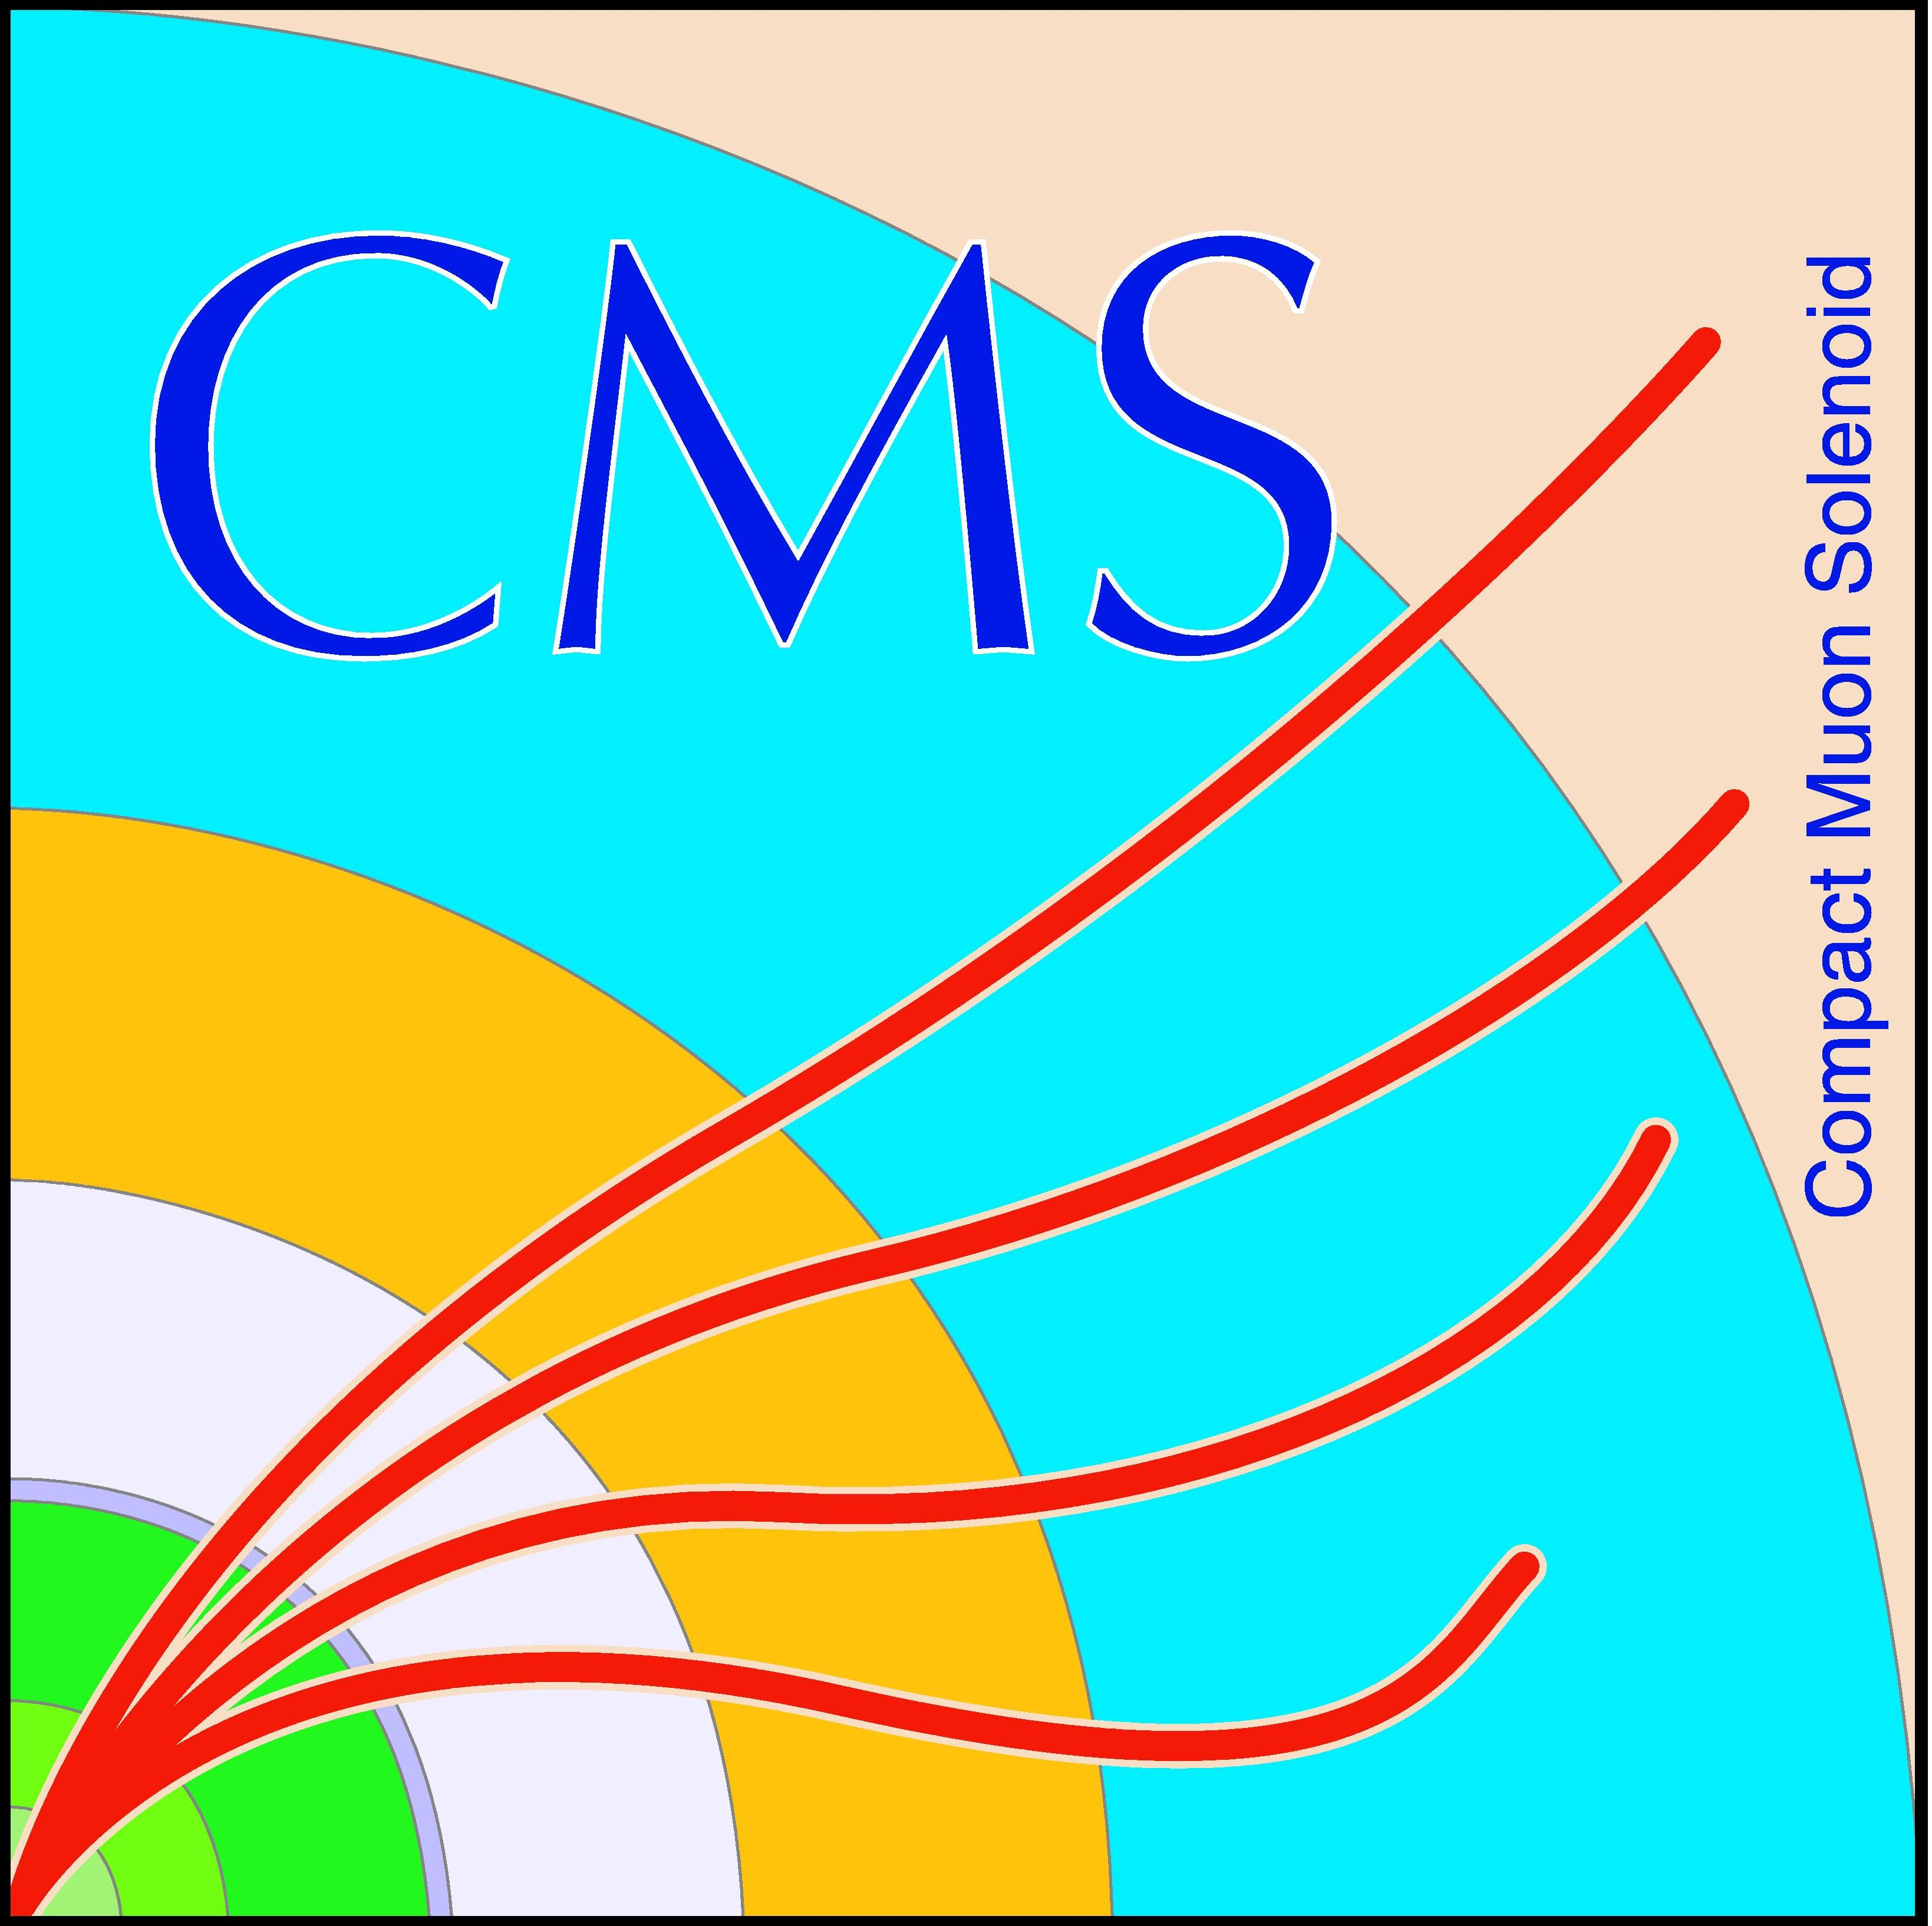
\includegraphics[height=1.5cm]{CMSlogo.jpeg}
  \end{center}
}

% pdflatex packages
\hypersetup{bookmarks=true}
\hypersetup{unicode=false}
\hypersetup{pdftitle={Lost-Lepton}}
\hypersetup{pdfauthor={Arne-Rasmus~Dr\"ager}}


\begin{document}
% ==================================================
% --------------------------------------------------
\begin{frame}
  \titlepage
\end{frame}
\section{Lost-Lepton Method}
\begin{frame}
 \begin{block}{}
 \centering
 \Large Lost-Lepton Background Concept
 \end{block}
\end{frame}

\begin{frame}
\frametitle{Outline}
\normalsize
\begin{itemize}
 \item Reminder: The lost-lepton background is estimated selecting a single $\mu$/e control-sample and weighting each event according to the lepton efficiencies
 \item The following slides illustrate the lost-lepton background composition and the full picture of the estimation method
 \begin{itemize}
 \item Slides 4,5: Simple case for only lost $\mu$ using a single $\mu$ control-sample
 \item Slides 6,7: Adding the lost electrons, still using only the single $\mu$ control-sample
 \item Slides 8: Same as slide 7 but using now the single electron control-sample
  \end{itemize}
  \item The final prediction of the lost-lepton method is a combination of the statistical uncorrelated predictions using the single electron and single muon control-sample
\end{itemize}
\end{frame}

\begin{frame}
\frametitle{Lost-Lepton Background $\mu$ only}
 \begin{center}
 \begin{overpic}[width=1.0\textwidth]{figures/Sketches/LostLeptonSketch.pdf} \end{overpic}
 \end{center}
\end{frame}

\begin{frame}
\frametitle{Lost-Lepton Background $\mu$ only}
 \begin{center}
 \begin{overpic}[width=0.9\textwidth]{figures/Sketches/LostLeptonSketch_mu_pred.pdf} 
 \put(0,10){\rotatebox{-0}{\normalsize Expectation \& Prediction using single $\mu$ control-sample (CS)}}
 \end{overpic}

 \end{center}
\end{frame}


\begin{frame}
\frametitle{Lost-Lepton Background $\mu$ \& e}
 \begin{center}
 \begin{overpic}[width=0.9\textwidth]{figures/Sketches/LostLeptonSketch_ll.pdf} 
%  \put(0,10){\rotatebox{-0}{\normalsize Expectation \& Prediction using single $\mu$ control sample (CS)}}
 \end{overpic}

 \end{center}
\end{frame}


\begin{frame}
\frametitle{Lost-Lepton Background $\mu$ \& e}
 \begin{center}
 \begin{overpic}[width=0.80\textwidth]{figures/Sketches/LostLeptonSketch_mu_pred_full.pdf} 
  \put(0,-3){\rotatebox{-0}{\normalsize Expectation \& Prediction using single $\mu$ control-sample (CS)}}
 \end{overpic}

 \end{center}
\end{frame}

\begin{frame}
\frametitle{Lost-Lepton Background $\mu$ \& e}
 \begin{center}
 \begin{overpic}[width=0.80\textwidth]{figures/Sketches/LostLeptonSketch_e_pred_full.pdf} 
  \put(0,-3){\rotatebox{-0}{\normalsize Expectation \& Prediction using single e control-sample (CS)}}
 \end{overpic}

 \end{center}
\end{frame}

\subsection{Lost-Lepton Closure}
\begin{frame}
 \begin{block}{}
 \centering
 \Large Lost-Lepton Closure Test: Status
 \end{block}


\end{frame}

\begin{frame}
  \begin{columns}
    \begin{column}{0.5\textwidth}
     \centering
      \begin{overpic}[width=0.57\textwidth]{figures/Closure/Baseline/Closure__HT__MCEx_vs_MuPrMTWDiLep+ElecPrMTWDiLep__Baseline.pdf}
%              \put(64,84){\rotatebox{-0}{\tiny Work in progress}}
     \end{overpic}
           \begin{overpic}[width=0.57\textwidth]{figures/Closure/Baseline/Closure__MHT__MCEx_vs_MuPrMTWDiLep+ElecPrMTWDiLep__Baseline.pdf}
%            \put(64,84){\rotatebox{-0}{\tiny Work in progress}}
     \end{overpic}
    \end{column}
    \begin{column}{0.5\textwidth}
      \centering
           \begin{overpic}[width=0.57\textwidth]{figures/Closure/Baseline/Closure__NJets__MCEx_vs_MuPrMTWDiLep+ElecPrMTWDiLep__Baseline.pdf}
%             \put(64,84){\rotatebox{-0}{\tiny Work in progress}}
     %     \put(90,90){\rotatebox{-45}{\scriptsize \Large Arne}}
     \end{overpic}
     \begin{overpic}[width=0.57\textwidth]{figures/Closure/Baseline/Closure__BTags__MCEx_vs_MuPrMTWDiLep+ElecPrMTWDiLep__Baseline.pdf}
% \put(64,84){\rotatebox{-0}{\tiny Work in progress}}
      \end{overpic}
    \end{column}
  \end{columns}
   \begin{itemize}
  \item Using full method combining electron and muon prediction. Applying correction for isoalated track veto.
 \end{itemize}
\end{frame}
\begin{frame}
\begin{center}
  \begin{overpic}[width=0.60\textwidth]{figures/Closure/Baseline/Closure__Bin__MCEx_vs_MuPrMTWDiLep+ElecPrMTWDiLep__Baseline.pdf}
%              \put(64,84){\rotatebox{-0}{\tiny Work in progress}}
     \end{overpic}
\end{center}
\begin{itemize}
 \item No Isolated Track:  Exp: $3619.4 \pm 18.0$ Pred: $3511.0 \pm 10.8$
  \item With Isolated Track:  Exp: $2976.7 \pm 16.3$ Pred: $2884.8 \pm 7.9$ (shown)
\end{itemize}

\end{frame}
\begin{frame}
\frametitle{Closure: $\mu$ CS only}
  \begin{columns}
    \begin{column}{0.33\textwidth}
     \centering
       \begin{overpic}[width=0.99\textwidth]{figures/Closure_Step_By_Step_Mu/Baseline_MuIso/Closure_Step_By_Step_Mu__Bin__MCEx_vs_MuCSMTWDiLepCorrected__Baseline_MuIso.pdf}
        
       \end{overpic}\\
\begin{overpic}[width=0.99\textwidth]{figures/Closure_Step_By_Step_Mu/Baseline_ElecAcc/Closure_Step_By_Step_Mu__Bin__MCEx_vs_MuCSMTWDiLepCorrected__Baseline_ElecAcc.pdf}
        
       \end{overpic}
    \end{column}
    \begin{column}{0.33\textwidth}
     \centering
  \begin{overpic}[width=0.99\textwidth]{figures/Closure_Step_By_Step_Mu/Baseline_MuReco/Closure_Step_By_Step_Mu__Bin__MCEx_vs_MuCSMTWDiLepCorrected__Baseline_MuReco.pdf}
        
       \end{overpic}\\
\begin{overpic}[width=0.99\textwidth]{figures/Closure_Step_By_Step_Mu/Baseline_ElecReco/Closure_Step_By_Step_Mu__Bin__MCEx_vs_MuCSMTWDiLepCorrected__Baseline_ElecReco.pdf}
        
       \end{overpic}
    \end{column} 
    \begin{column}{0.33\textwidth}
     \centering
  \begin{overpic}[width=0.99\textwidth]{figures/Closure_Step_By_Step_Mu/Baseline_MuAcc/Closure_Step_By_Step_Mu__Bin__MCEx_vs_MuCSMTWDiLepCorrected__Baseline_MuAcc.pdf}
        
       \end{overpic}\\
\begin{overpic}[width=0.99\textwidth]{figures/Closure_Step_By_Step_Mu/Baseline_ElecIso/Closure_Step_By_Step_Mu__Bin__MCEx_vs_MuCSMTWDiLepCorrected__Baseline_ElecIso.pdf} 
       \end{overpic}
    \end{column}

  \end{columns}
\end{frame}

\begin{frame}
\frametitle{Closure: e CS only}
  \begin{columns}
    \begin{column}{0.33\textwidth}
     \centering
       \begin{overpic}[width=0.99\textwidth]{figures/Closure_Step_By_Step_Elec/Baseline_ElecIso/Closure_Step_By_Step_Elec__Bin__MCEx_vs_ElecCSMTWDiLepCorrected__Baseline_ElecIso.pdf}
        
       \end{overpic}\\
\begin{overpic}[width=0.99\textwidth]{figures/Closure_Step_By_Step_Elec/Baseline_MuAcc/Closure_Step_By_Step_Elec__Bin__MCEx_vs_ElecCSMTWDiLepCorrected__Baseline_MuAcc.pdf}
        
       \end{overpic}
    \end{column}
    \begin{column}{0.33\textwidth}
     \centering
  \begin{overpic}[width=0.99\textwidth]{figures/Closure_Step_By_Step_Elec/Baseline_ElecReco/Closure_Step_By_Step_Elec__Bin__MCEx_vs_ElecCSMTWDiLepCorrected__Baseline_ElecReco.pdf}
        
       \end{overpic}\\
\begin{overpic}[width=0.99\textwidth]{figures/Closure_Step_By_Step_Elec/Baseline_MuReco/Closure_Step_By_Step_Elec__Bin__MCEx_vs_ElecCSMTWDiLepCorrected__Baseline_MuReco.pdf}
        
       \end{overpic}
    \end{column} 
    \begin{column}{0.33\textwidth}
     \centering
  \begin{overpic}[width=0.99\textwidth]{figures/Closure_Step_By_Step_Elec/Baseline_ElecAcc/Closure_Step_By_Step_Elec__Bin__MCEx_vs_ElecCSMTWDiLepCorrected__Baseline_ElecAcc.pdf}
        
       \end{overpic}\\
\begin{overpic}[width=0.99\textwidth]{figures/Closure_Step_By_Step_Elec/Baseline_MuIso/Closure_Step_By_Step_Elec__Bin__MCEx_vs_ElecCSMTWDiLepCorrected__Baseline_MuIso.pdf} 
       \end{overpic}
    \end{column}

  \end{columns}
\end{frame}
\begin{frame}
\frametitle{Single e \& $\mu$ CS vs Expected events for 4 \fb}
\begin{center}
  \begin{overpic}[width=0.60\textwidth]{figures/CS_VS_Expectation/Baseline/CS_VS_Expectation__Bin__MCExTotal_vs_MCMuCS+MCElecCS__Baseline.pdf}
%              \put(64,84){\rotatebox{-0}{\tiny Work in progress}}
     \end{overpic}
     \begin{itemize}
      \item Overall for two CS events one lost-lepton
      \item Many bins with less than 1 CS event expected for 4 \fb
     \end{itemize}

\end{center}
\end{frame}


\subsection{Lost-Lepton Tag \& Probe}
\begin{frame}
 \begin{block}{}
 \centering
 \Large Lost-Lepton Tag \& Probe
 \end{block}

\end{frame}

\section{Tag \& Probe}
\subsection{Setup}
\begin{frame}
%  \frametitle{Mini Isolation (UCSB approach \href{https://indico.cern.ch/event/368826/contribution/3/material/slides/0.pdf}{Adam talk}) vs Classical Isolation}
\frametitle{Lepton Definition}
\begin{itemize}
 \item Muon:
 \begin{itemize}
  \item Reco/ID: "Tight" ID
  \item Iso: Mini Isolation: Max Cone: 0.2 Min Cone: 0.05 $\delta \beta I(rel)<0.2$
 \end{itemize}
  \item Electron:
 \begin{itemize}
  \item Reco/ID: "Veto" ID
  \item Iso: Mini Isolation: Max Cone: 0.2 Min Cone: 0.05 $\delta \beta I(rel)<0.1$
 \end{itemize}
 \item Tag \& Probe:
 \begin{itemize}
 \item ID:
 \begin{itemize}
  \item Tag: Iso muon(Electron)
  \item Probe: slimmedMuons(slimmedElectrons) $\rightarrow$ Reco/ID muon(electron)
  \item Improve probe: Use Superclusters photons (for electrons) but miniAOD stores only above  14 GeV
  \item Improve probe: Could use tracks (for muons) but very high background
 \end{itemize}
  \item Iso:
 \begin{itemize}
  \item Tag: Iso muon(Electron)
  \item Probe: Reco/ID muon(electron) $\rightarrow$ Iso muon(electron)
  
 \end{itemize}

 \end{itemize}
\end{itemize}
\end{frame}
\begin{frame}
 \frametitle{Tag \& Probe technicals}
 \begin{itemize}
  \item Test Several cuts to increase kinematical similarity to search region
  \begin{itemize}
   \item $\HT>500,400,200 \gev$
   \item $\mindeltaphi >4.0, No Cut$ (Treat Tag leptons \pt as neutrino \pt $\rightarrow$ \MHT)
   \item $\NJets\geq4$
  \end{itemize}

  \item Apply $\HT>500$ \& $\NJets\geq4$ (similar kinematics to baseline region)
  \item Select (randomly) tag lepton from isolated lepton collection
  \item Select all probe leptons except matched to tag
  \item Compute for all invariant mass (Z mass)
  \item Check property (ID/iso criteria)
  \item Use electroweak code for fitting and eff. determination
  \begin{itemize}
   \item Fit function: gaussPlusCubic
  \end{itemize}

 \end{itemize}
\end{frame}

\begin{frame}
 \frametitle{Comparison \ttbar \& \wpj vs DY (truth) Efficiencies}
  \begin{columns}

   \begin{column}{0.33\textwidth}
     \begin{itemize}
   \item $\mu$ Iso \ttbar \& \wpj eff. (truth info.)
  \end{itemize}
    \begin{tikzpicture}
    \node[anchor=south west,inner sep=0] (image) at (0,0) {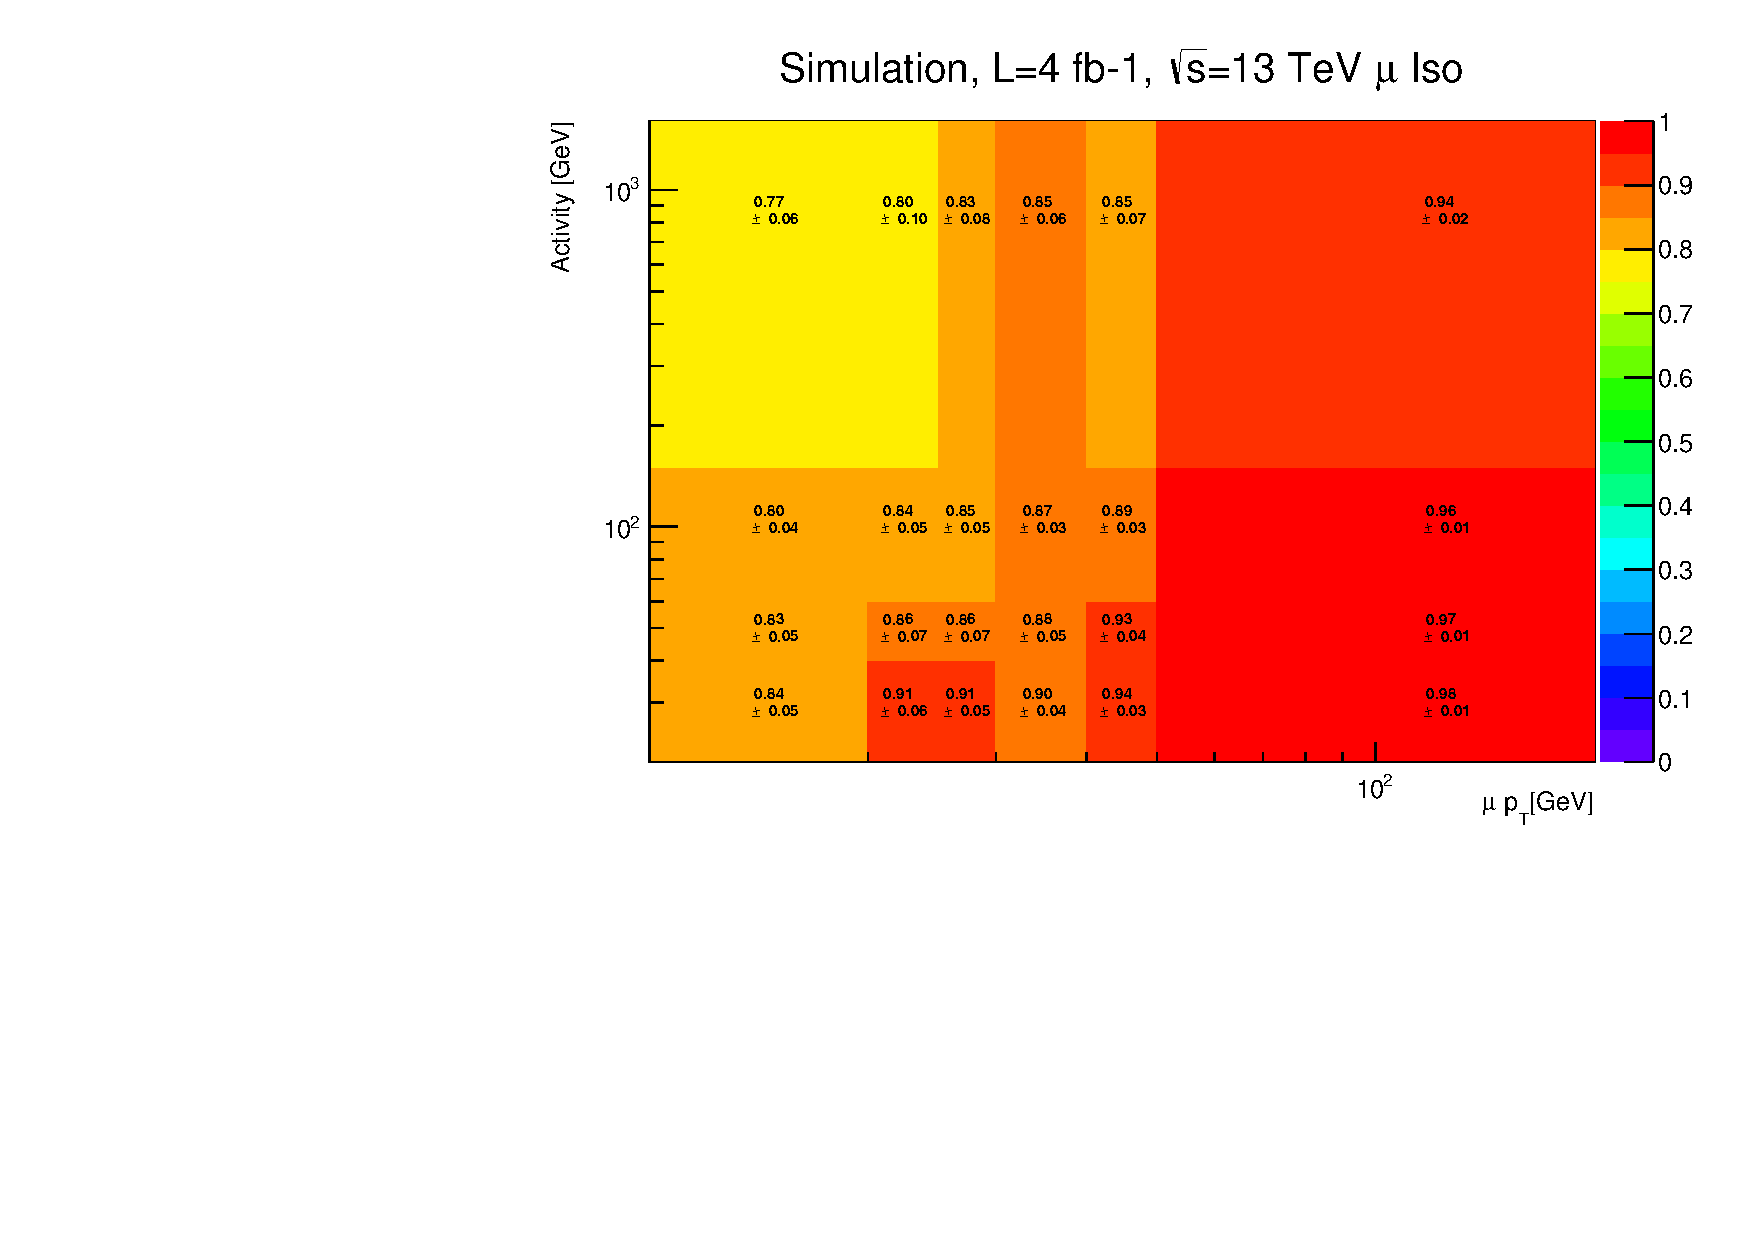
\includegraphics[width=1.\textwidth]{figures/efficiencies/MuIsoPTActivity_ttbarWPJ.pdf}};
    \begin{scope}[x={(image.south east)},y={(image.north west)}]
%         \draw[red,ultra thick,rounded corners] (0.62,0.65) rectangle (0.78,0.75);
%         \draw[red,ultra thick,rounded corners] (0.60,0.01) rectangle (0.75,0.99); % cordinates unten links(x,y) oben rechts(x,y)
    \end{scope}
   \end{tikzpicture}
   \end{column}
   \begin{column}{0.33\textwidth}
   \begin{itemize}
    \item $\mu$ Iso DY eff. \\(truth info.)
   \end{itemize}

    \begin{tikzpicture}
    \node[anchor=south west,inner sep=0] (image) at (0,0) {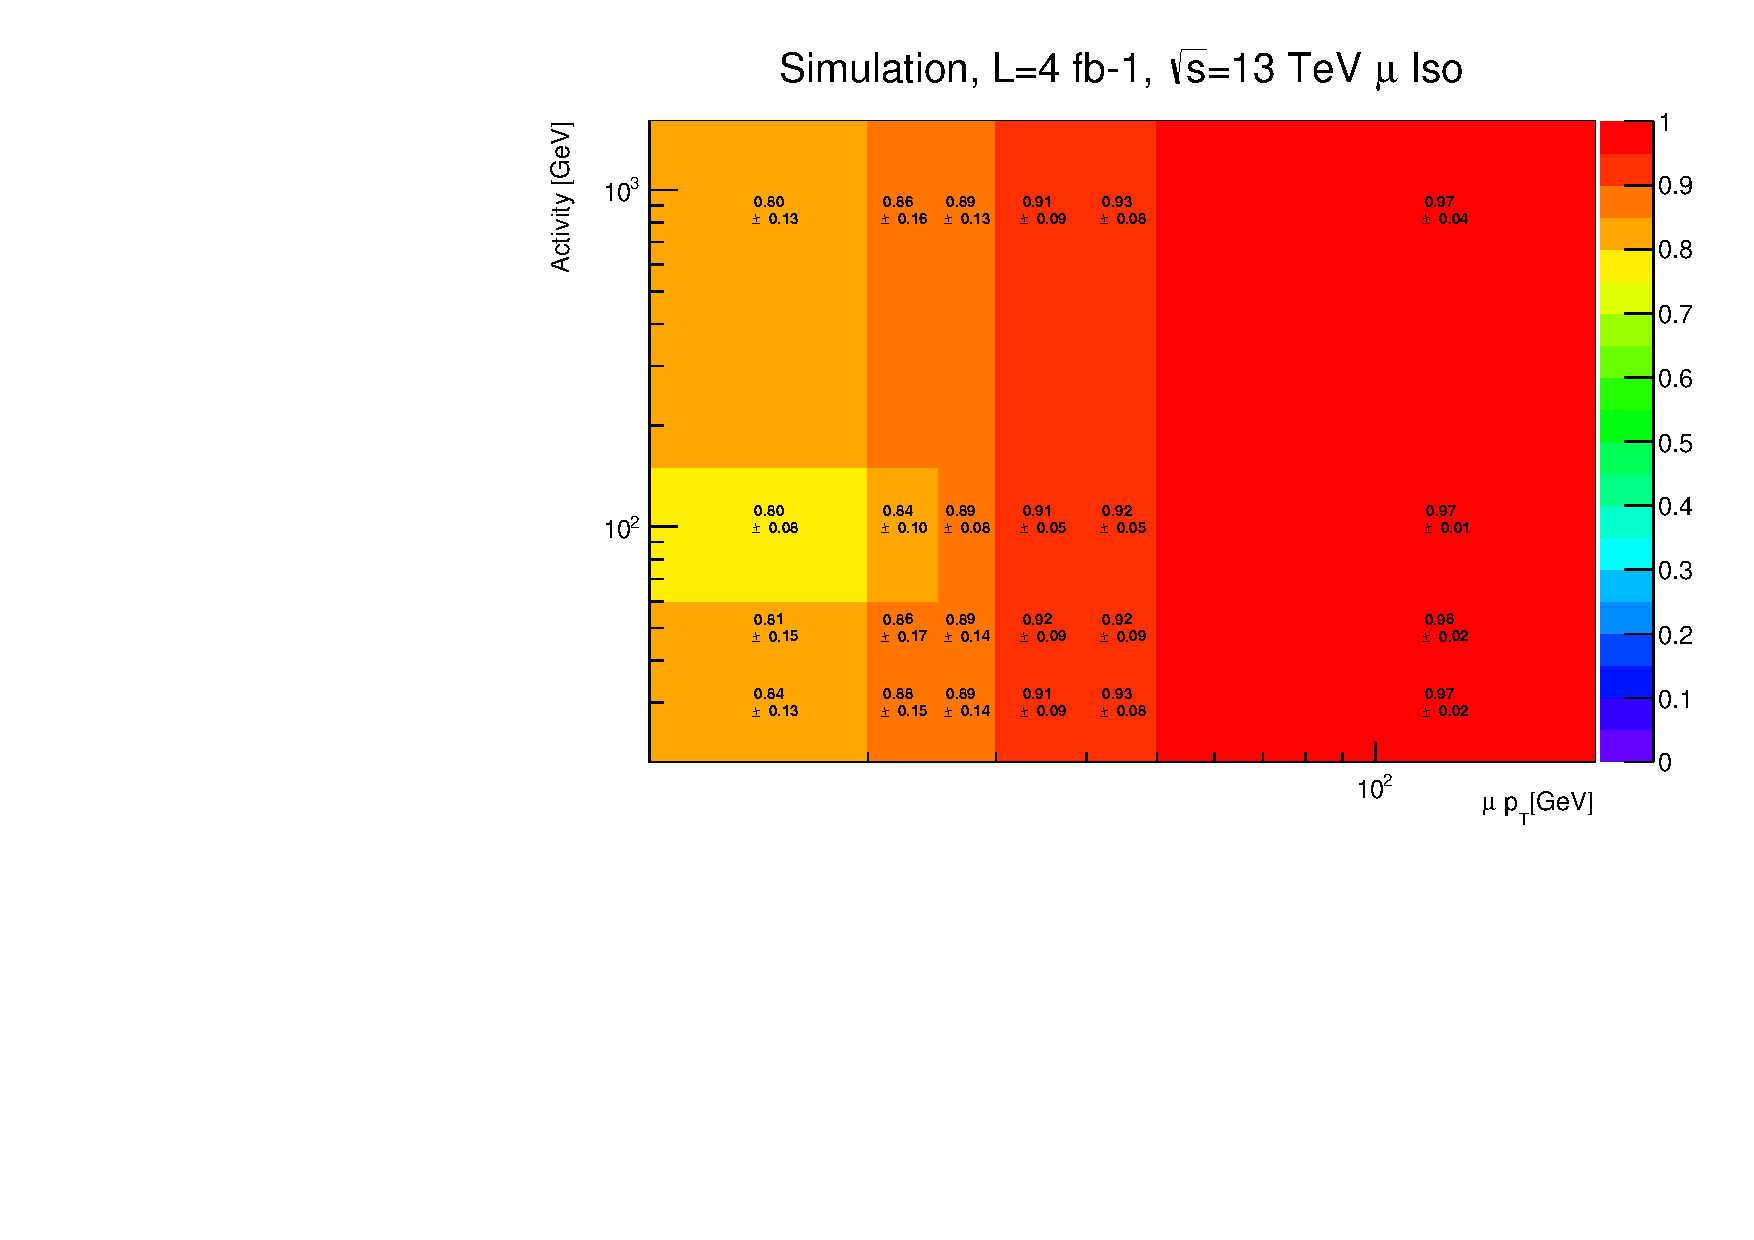
\includegraphics[width=1.\textwidth]{figures/efficiencies/MuIsoPTActivity_DY_noTagAndProbe.pdf}};
    \begin{scope}[x={(image.south east)},y={(image.north west)}]
%         \draw[red,ultra thick,rounded corners] (0.62,0.65) rectangle (0.78,0.75);
%         \draw[red,ultra thick,rounded corners] (0.60,0.01) rectangle (0.75,0.99); % cordinates unten links(x,y) oben rechts(x,y)
    \end{scope}
   \end{tikzpicture}
   \end{column}
           \begin{column}{0.33\textwidth}
   \begin{itemize}
    \item $\mu$ iso radio
   \end{itemize}

    \begin{tikzpicture}
     \node[anchor=south west,inner sep=0] (image) at (0,0) {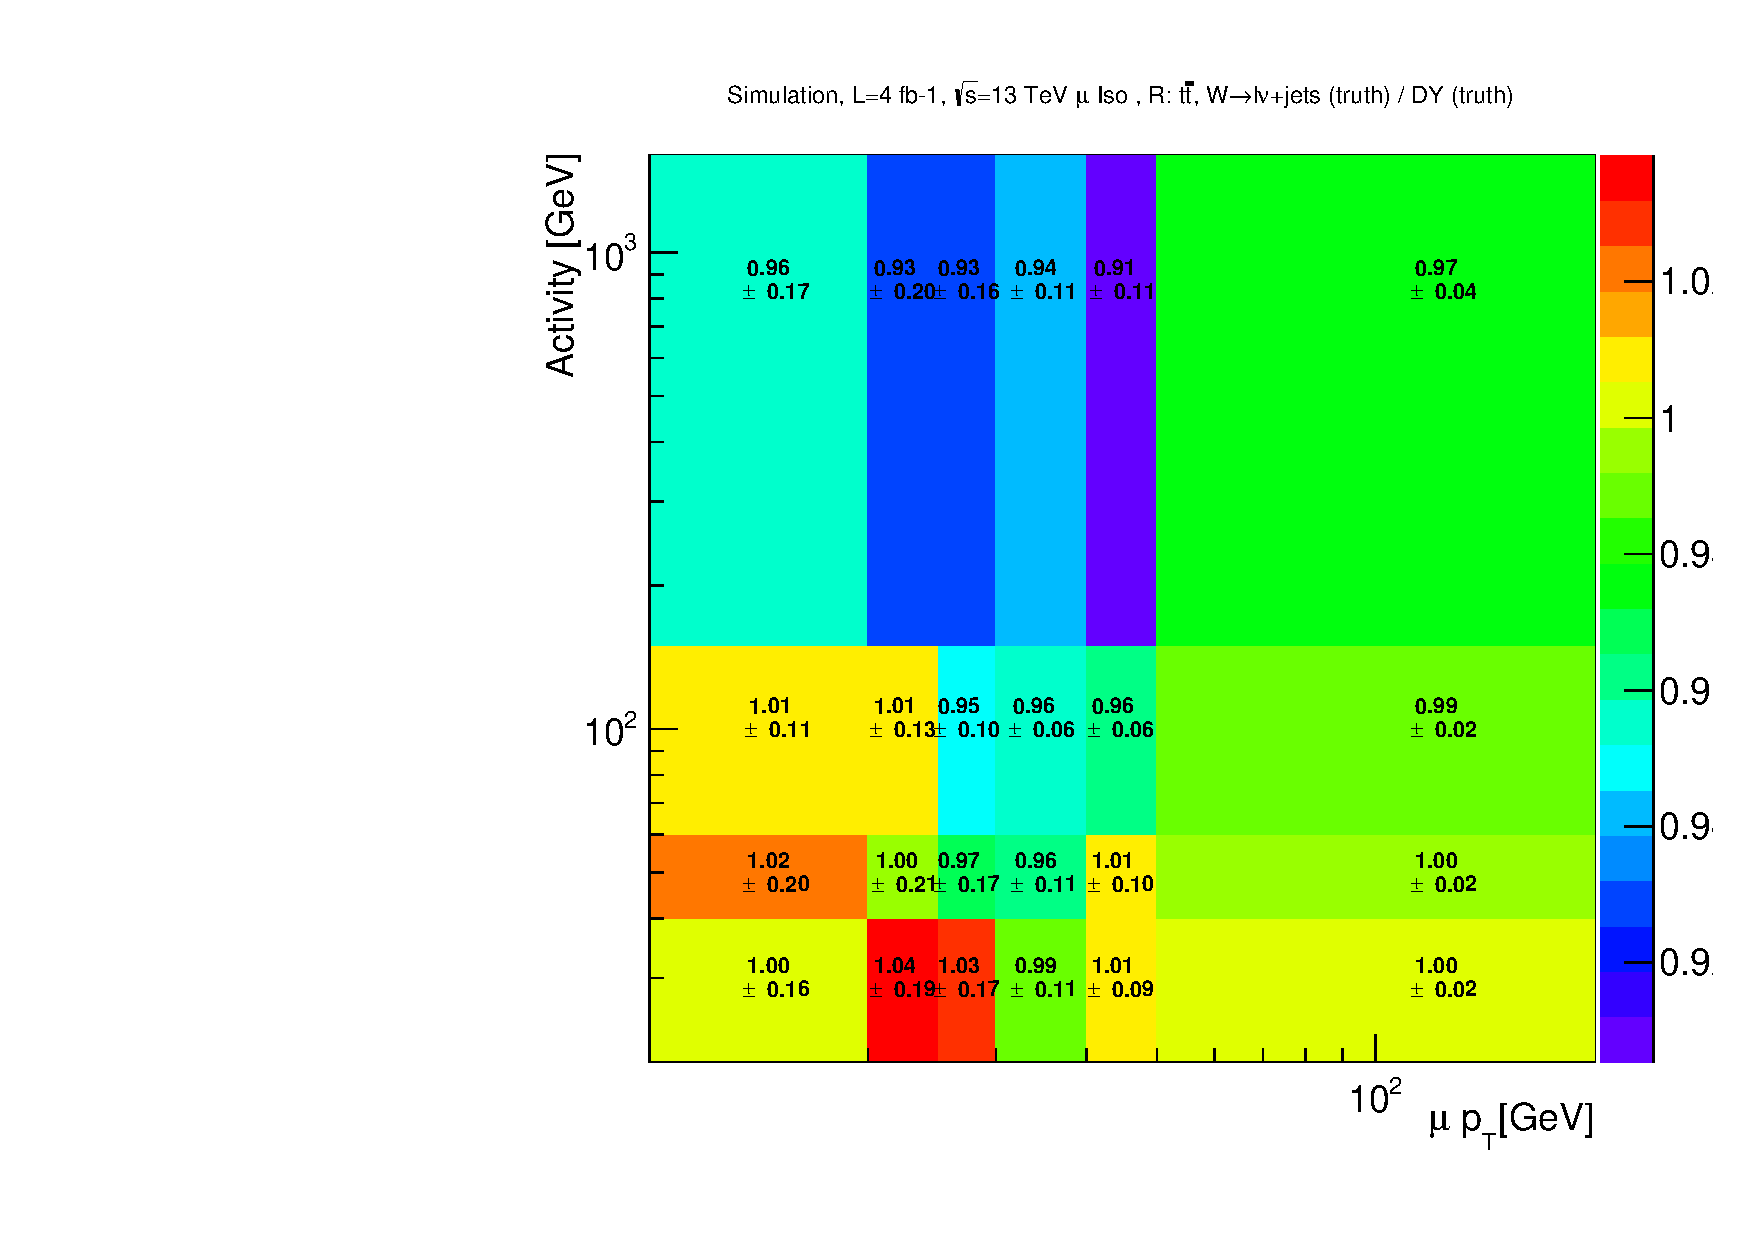
\includegraphics[width=1.\textwidth]{figures/efficiencies/ttbarwpjToTruthDY/MuIsoPTActivity_ratio.pdf}};
    \begin{scope}[x={(image.south east)},y={(image.north west)}]
%         \draw[red,ultra thick,rounded corners] (0.62,0.65) rectangle (0.78,0.75);
%         \draw[red,ultra thick,rounded corners] (0.60,0.01) rectangle (0.75,0.99); % cordinates unten links(x,y) oben rechts(x,y)
    \end{scope}
   \end{tikzpicture}
   \end{column}
  \end{columns}
\begin{itemize}
 \item Efficiencies obtained (using truth information) from \ttbar \& \wpj and DY are in good agreement 
 \item Lepton \pt and Activity are suffiantly topology independent to be transfered from DY to signal region!
 \item Check agreement using a Tag\&Probe method
\end{itemize}
\end{frame}

\begin{frame}
 \frametitle{Comparison \ttbar \& \wpj vs DY Tag \& Probe Efficiencies}
   \begin{columns}

   \begin{column}{0.33\textwidth}
     \begin{itemize}
   \item $\mu$ Iso \ttbar \& \wpj eff. (truth info.)
  \end{itemize}
    \begin{tikzpicture}
    \node[anchor=south west,inner sep=0] (image) at (0,0) {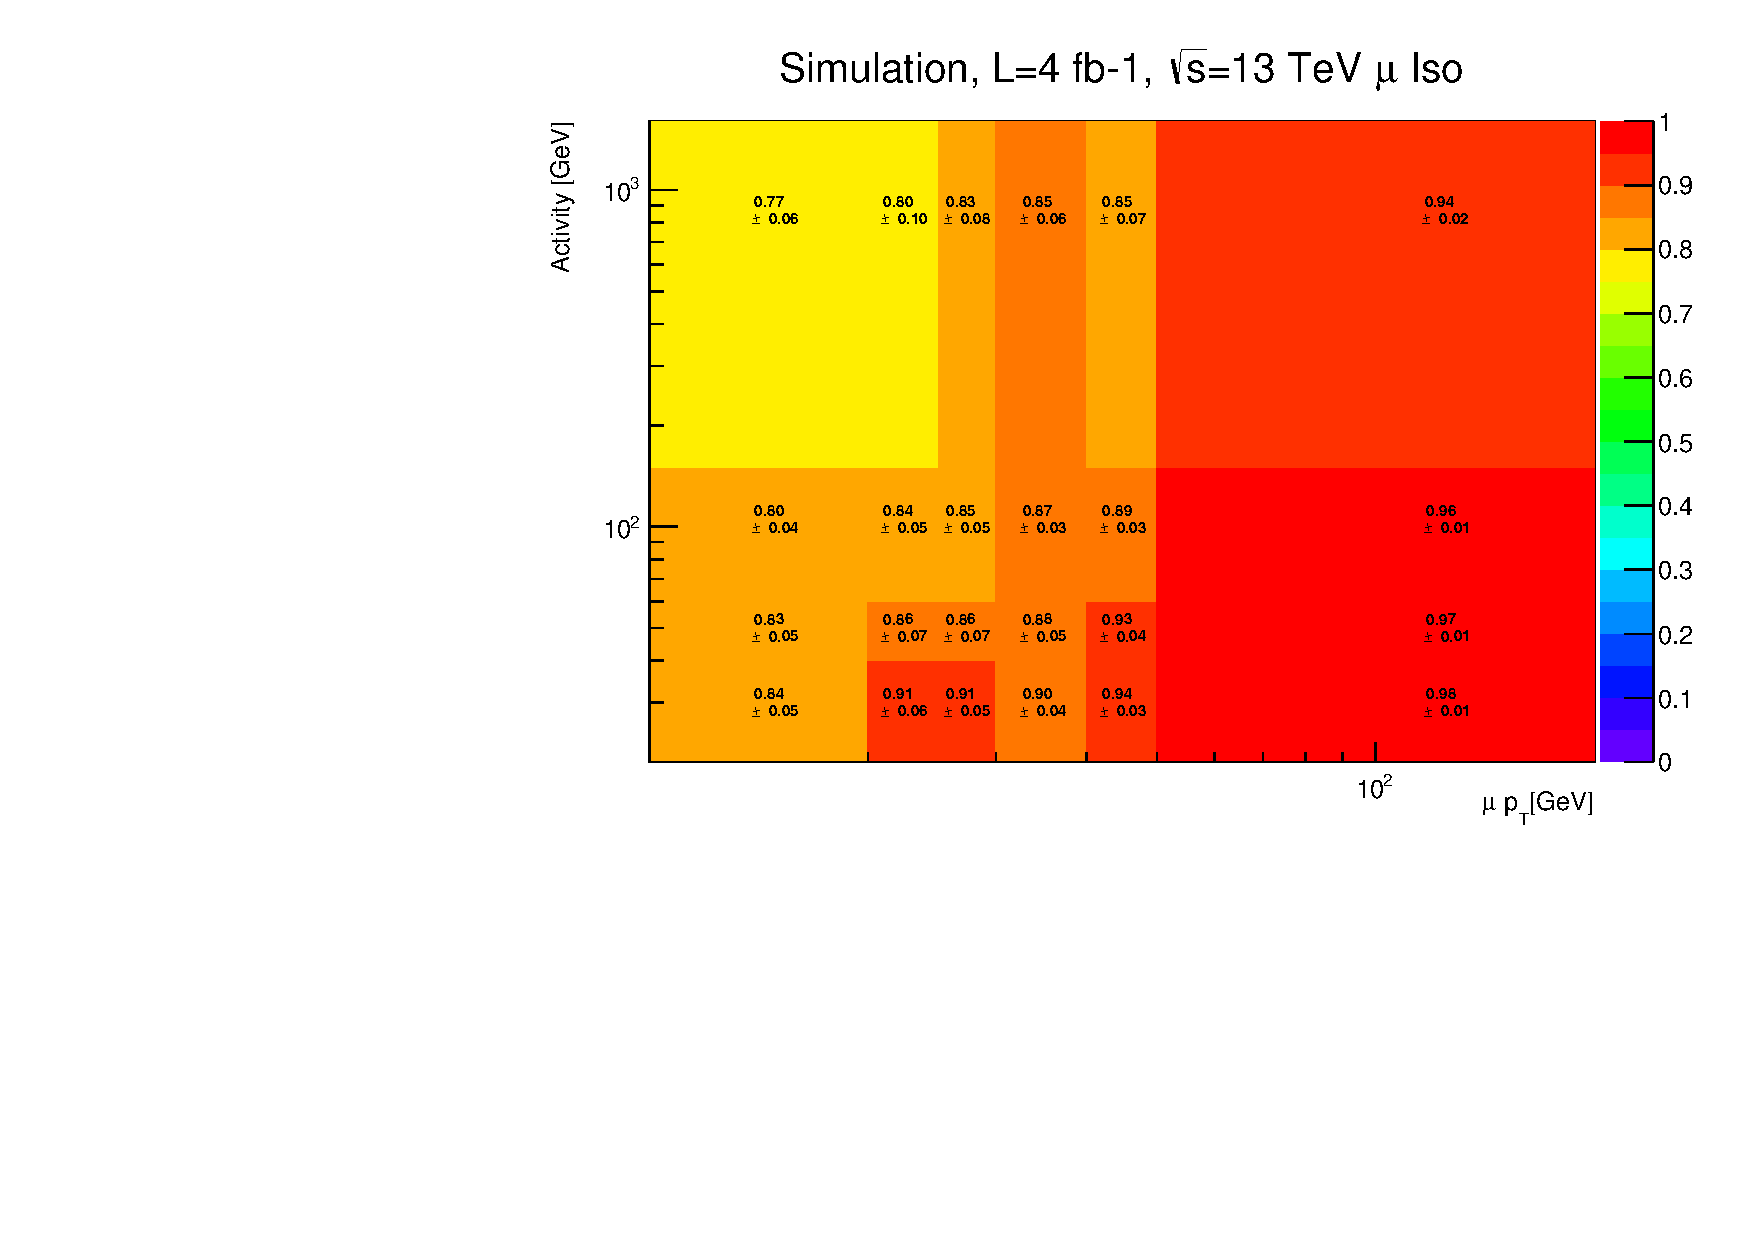
\includegraphics[width=1.\textwidth]{figures/efficiencies/MuIsoPTActivity_ttbarWPJ.pdf}};
    \begin{scope}[x={(image.south east)},y={(image.north west)}]
%         \draw[red,ultra thick,rounded corners] (0.62,0.65) rectangle (0.78,0.75);
%         \draw[red,ultra thick,rounded corners] (0.60,0.01) rectangle (0.75,0.99); % cordinates unten links(x,y) oben rechts(x,y)
    \end{scope}
   \end{tikzpicture}
   \end{column}
   \begin{column}{0.33\textwidth}
   \begin{itemize}
    \item $\mu$ Iso DY eff. \\(Tag \& Probe)
   \end{itemize}

    \begin{tikzpicture}
    \node[anchor=south west,inner sep=0] (image) at (0,0) {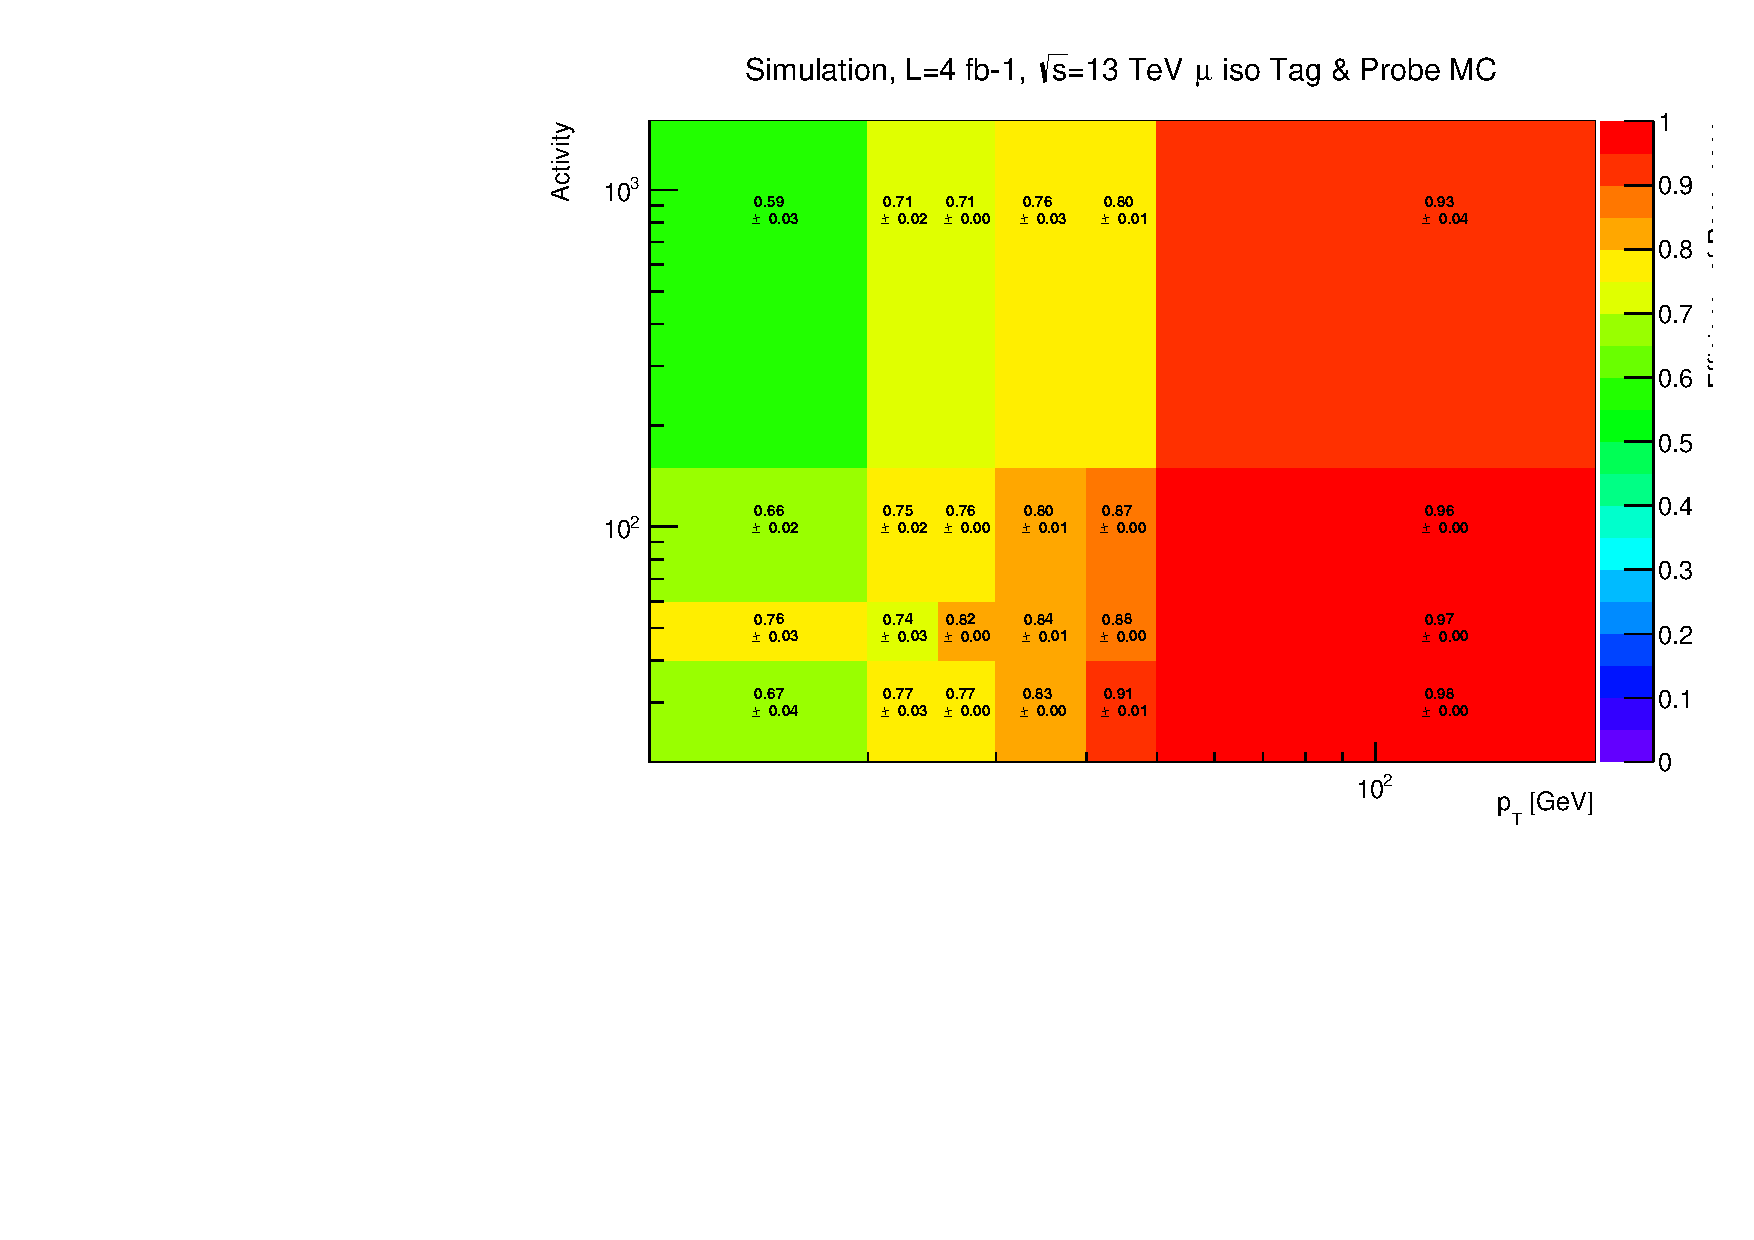
\includegraphics[width=1.\textwidth]{figures/efficiencies/MuIsoTagAndProbeMC.pdf}};
    \begin{scope}[x={(image.south east)},y={(image.north west)}]
%         \draw[red,ultra thick,rounded corners] (0.62,0.65) rectangle (0.78,0.75);
%         \draw[red,ultra thick,rounded corners] (0.60,0.01) rectangle (0.75,0.99); % cordinates unten links(x,y) oben rechts(x,y)
    \end{scope}
   \end{tikzpicture}
   \end{column}
           \begin{column}{0.33\textwidth}
   \begin{itemize}
    \item $\mu$ iso radio
   \end{itemize}

    \begin{tikzpicture}
     \node[anchor=south west,inner sep=0] (image) at (0,0) {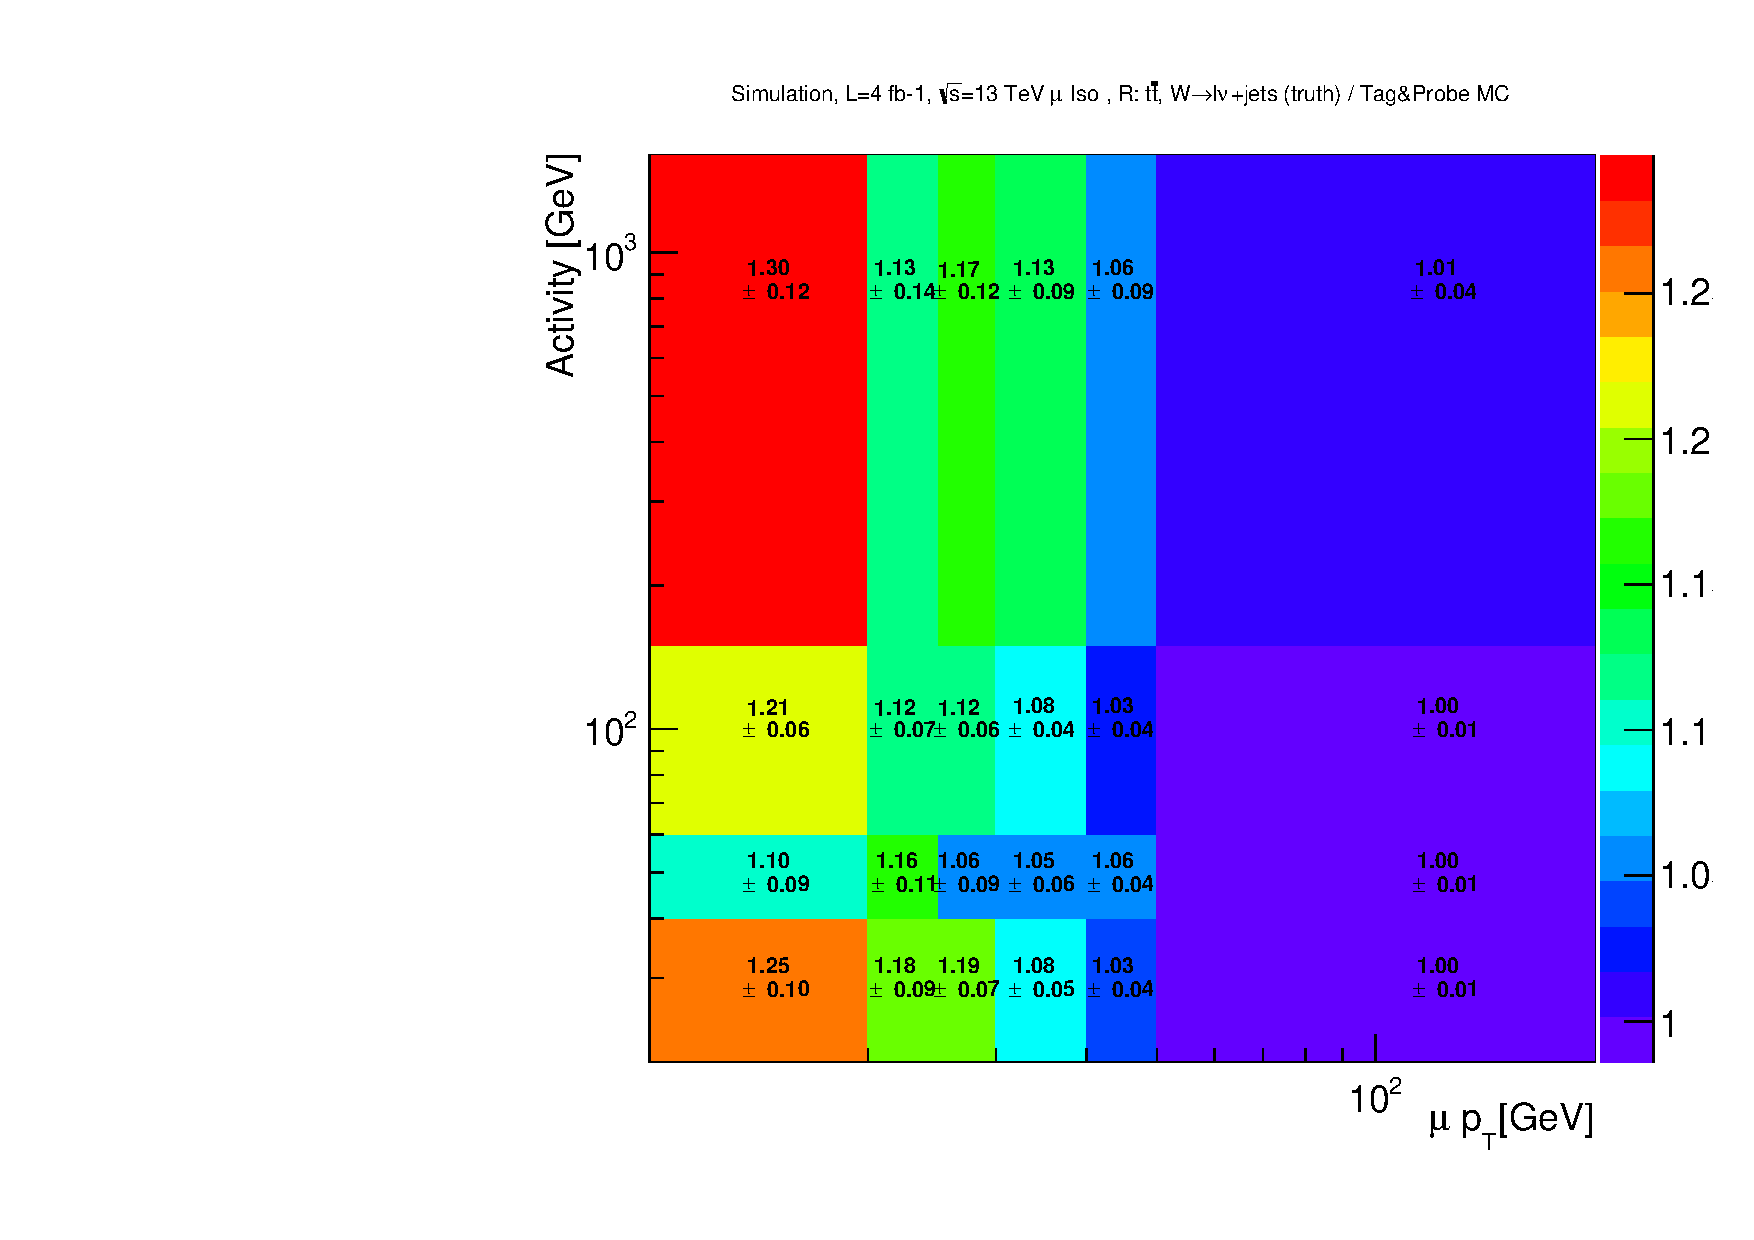
\includegraphics[width=1.\textwidth]{figures/efficiencies/tagandprobecompare/MuIsoPTActivity_ratio.pdf}};
    \begin{scope}[x={(image.south east)},y={(image.north west)}]
%         \draw[red,ultra thick,rounded corners] (0.62,0.65) rectangle (0.78,0.75);
%         \draw[red,ultra thick,rounded corners] (0.60,0.01) rectangle (0.75,0.99); % cordinates unten links(x,y) oben rechts(x,y)
    \end{scope}
   \end{tikzpicture}
   \end{column}
  \end{columns}
\begin{itemize}
 \item Efficiencies obtained via a Tag\&Probe method are significantly lower than efficiencies obtained using truth information
 \item Tag \& Probe Code \& Method needs to be checked for bugs
\end{itemize}
\end{frame}



% \begin{frame}
%  \frametitle{Resolve difference (idea)}
%  \begin{itemize}
%   \item \ttbar \& \wpj: Assume main source of \MHT neutrino from W decay
%   \item \Zll: Assume tag lepton to be reasonable equivalent to neutrino from W decay
%   \begin{itemize}
%    \item Calculate \mindeltaphi for tag lepton \pt
%   \end{itemize}
%  \end{itemize}
% \end{frame}
\begin{frame}
 \frametitle{Comparison \ttbar \& \wpj vs Tag \& Probe Efficiencies}
  \begin{columns}

   \begin{column}{0.33\textwidth}
     \begin{itemize}
   \item $\mu$ ID \ttbar \& \wpj eff. (truth info.)
  \end{itemize}
    \begin{tikzpicture}
    \node[anchor=south west,inner sep=0] (image) at (0,0) {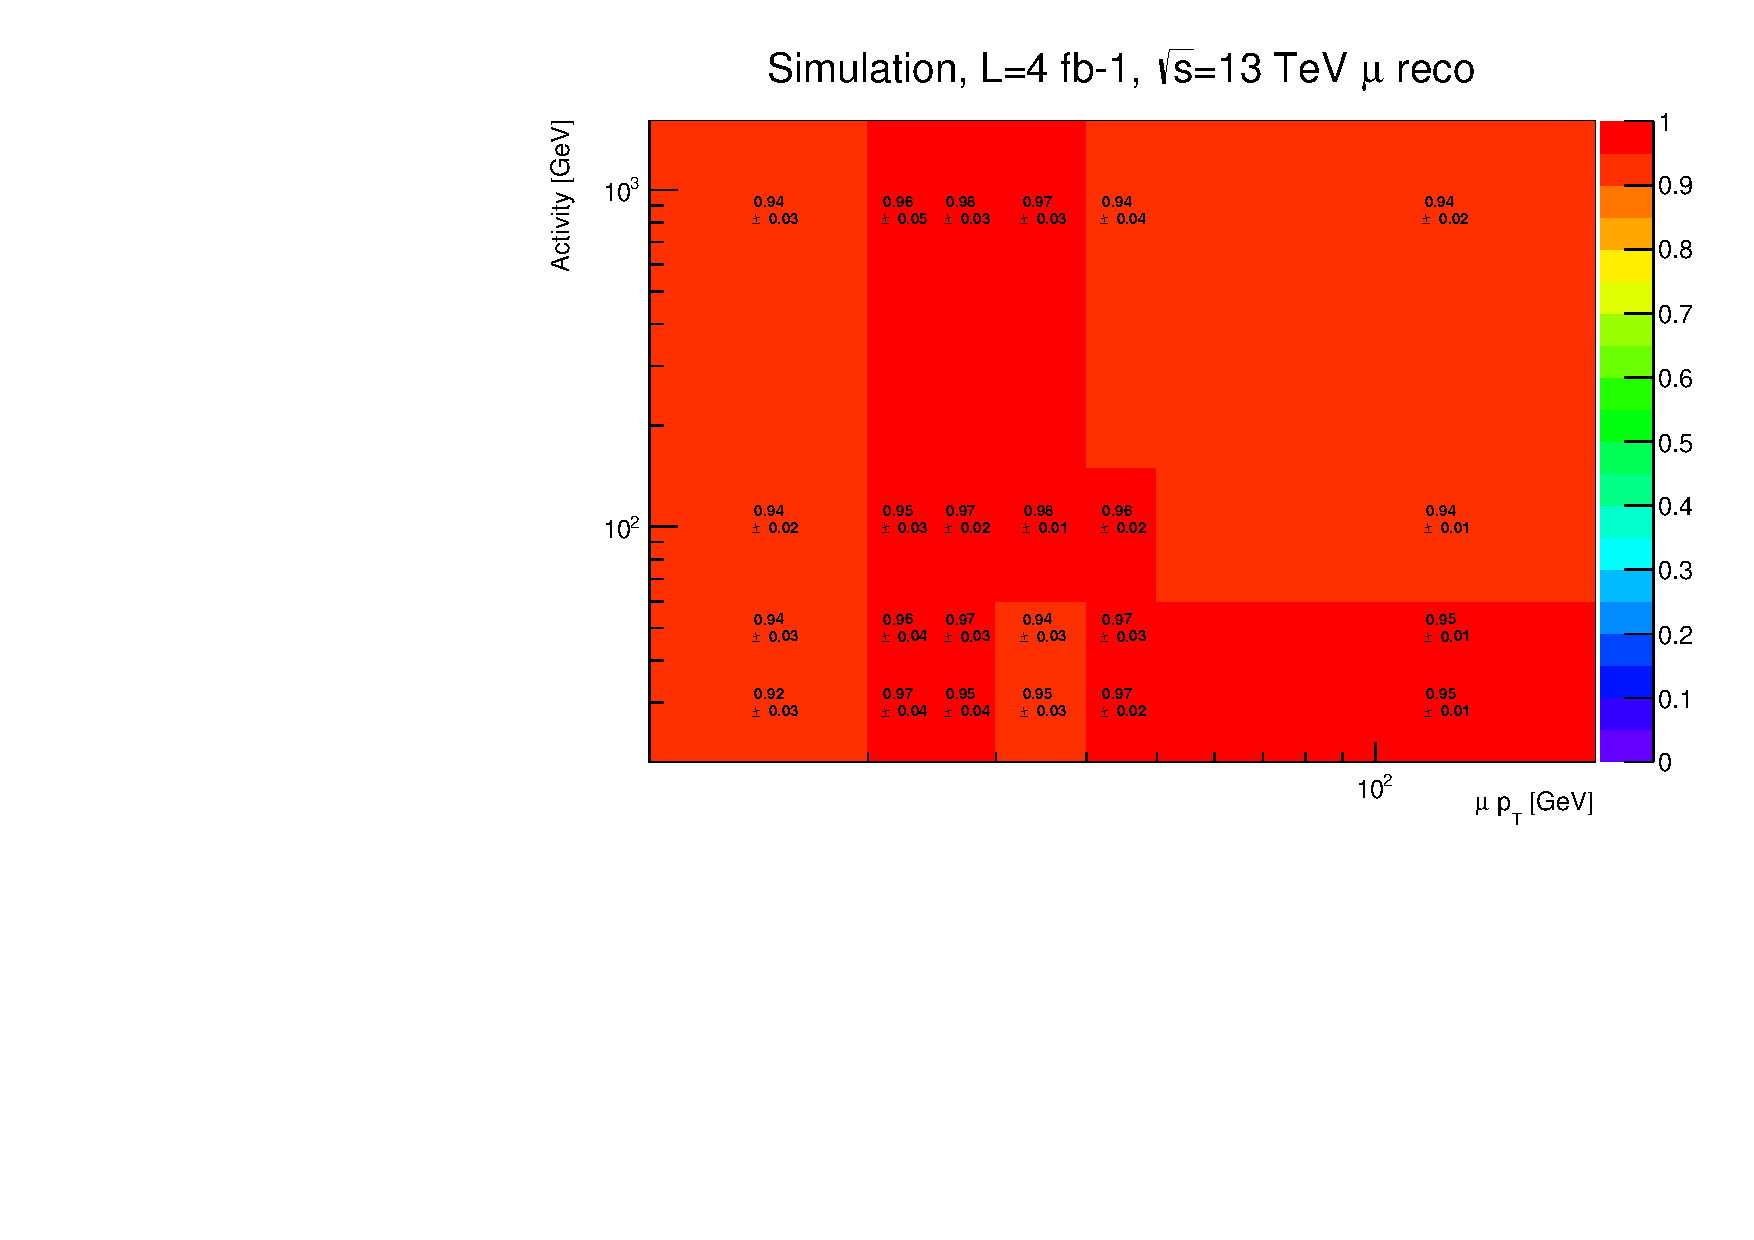
\includegraphics[width=1.\textwidth]{figures/efficiencies/MuRecoPTActivity_ttbarWPJ.pdf}};
    \begin{scope}[x={(image.south east)},y={(image.north west)}]
%         \draw[red,ultra thick,rounded corners] (0.62,0.65) rectangle (0.78,0.75);
%         \draw[red,ultra thick,rounded corners] (0.60,0.01) rectangle (0.75,0.99); % cordinates unten links(x,y) oben rechts(x,y)
    \end{scope}
   \end{tikzpicture}
   \end{column}
   \begin{column}{0.33\textwidth}
   \begin{itemize}
    \item $\mu$ ID DY eff.\\ (truth info.)
   \end{itemize}

    \begin{tikzpicture}
     \node[anchor=south west,inner sep=0] (image) at (0,0) {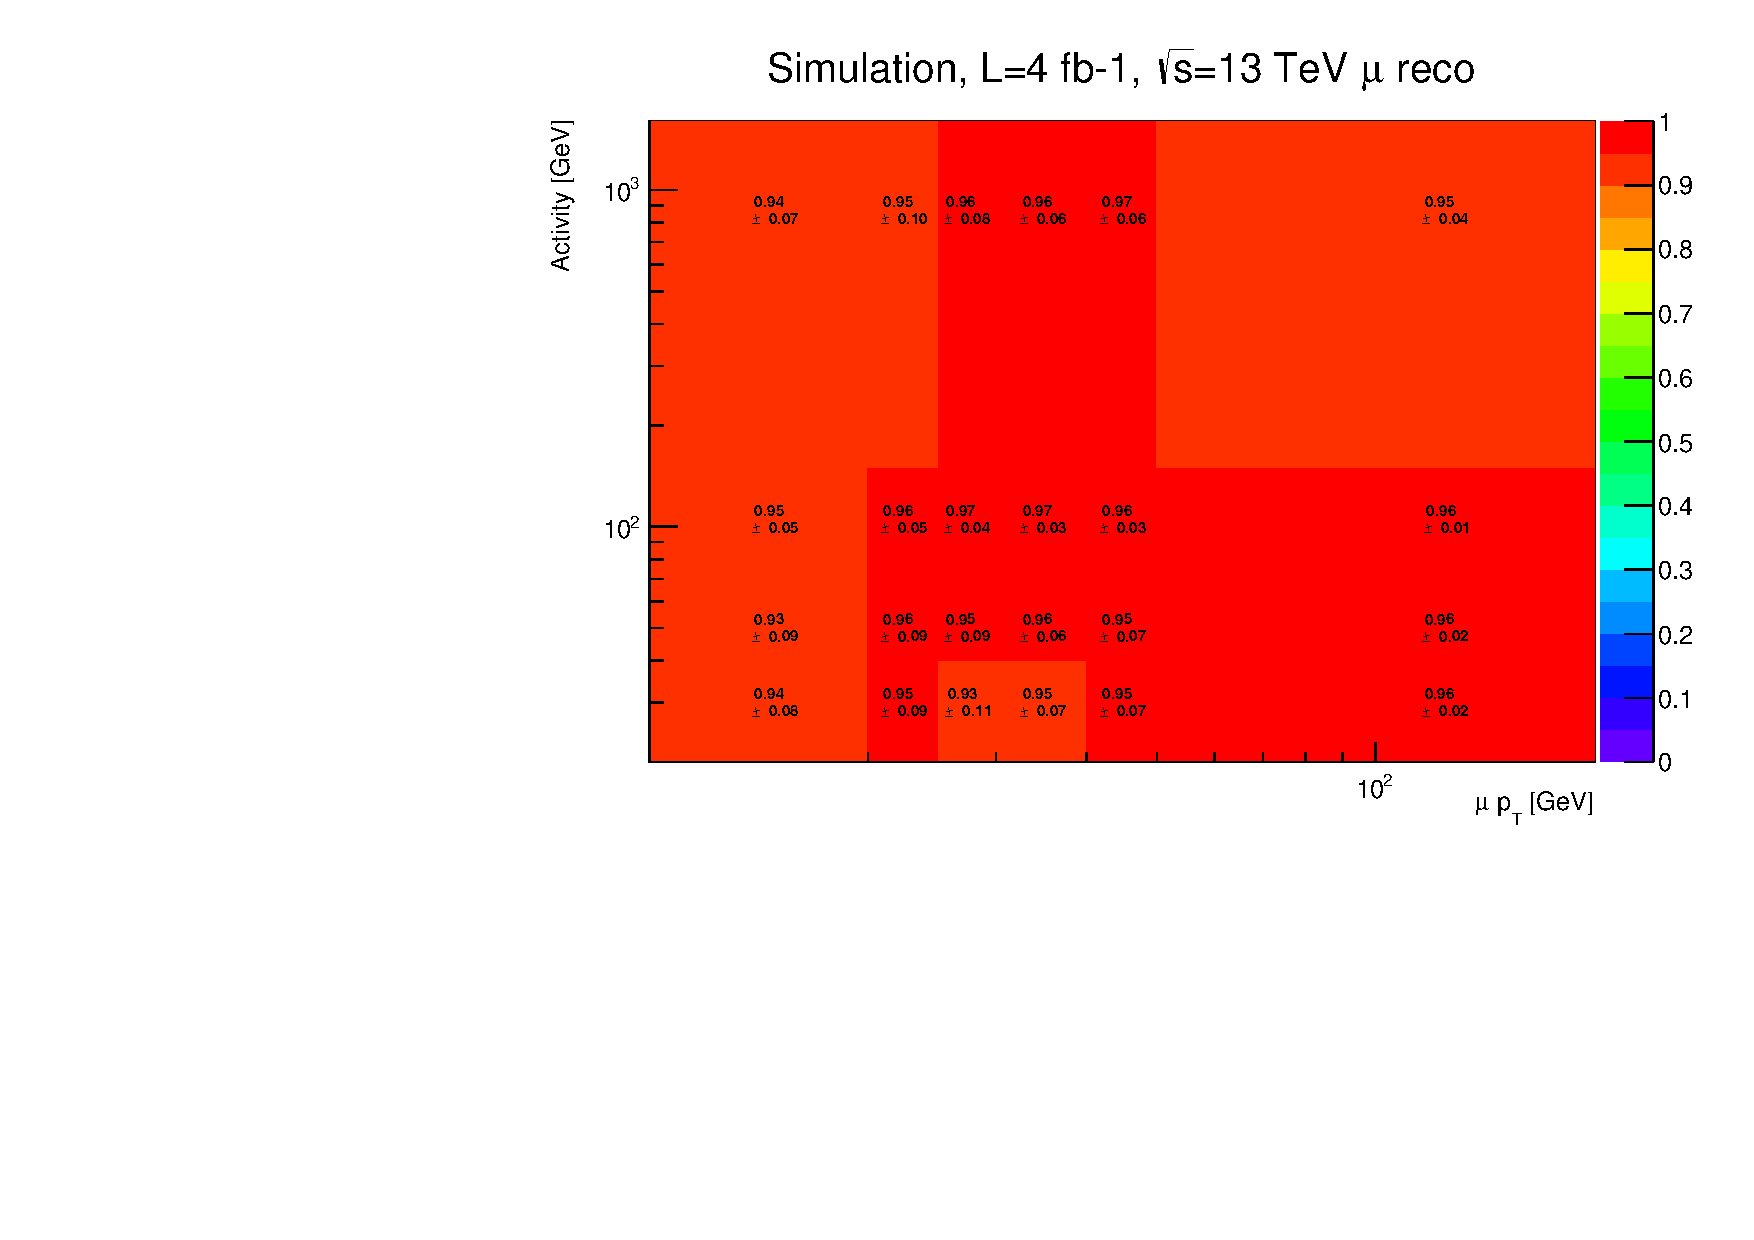
\includegraphics[width=1.\textwidth]{figures/efficiencies/MuRecoPTActivity_DY_noTagAndProbe.pdf}};
    \begin{scope}[x={(image.south east)},y={(image.north west)}]
%         \draw[red,ultra thick,rounded corners] (0.62,0.65) rectangle (0.78,0.75);
%         \draw[red,ultra thick,rounded corners] (0.60,0.01) rectangle (0.75,0.99); % cordinates unten links(x,y) oben rechts(x,y)
    \end{scope}
   \end{tikzpicture}
   \end{column}
        \begin{column}{0.33\textwidth}
   \begin{itemize}
    \item $\mu$ ID Tag \& Probe eff.
   \end{itemize}

    \begin{tikzpicture}
     \node[anchor=south west,inner sep=0] (image) at (0,0) {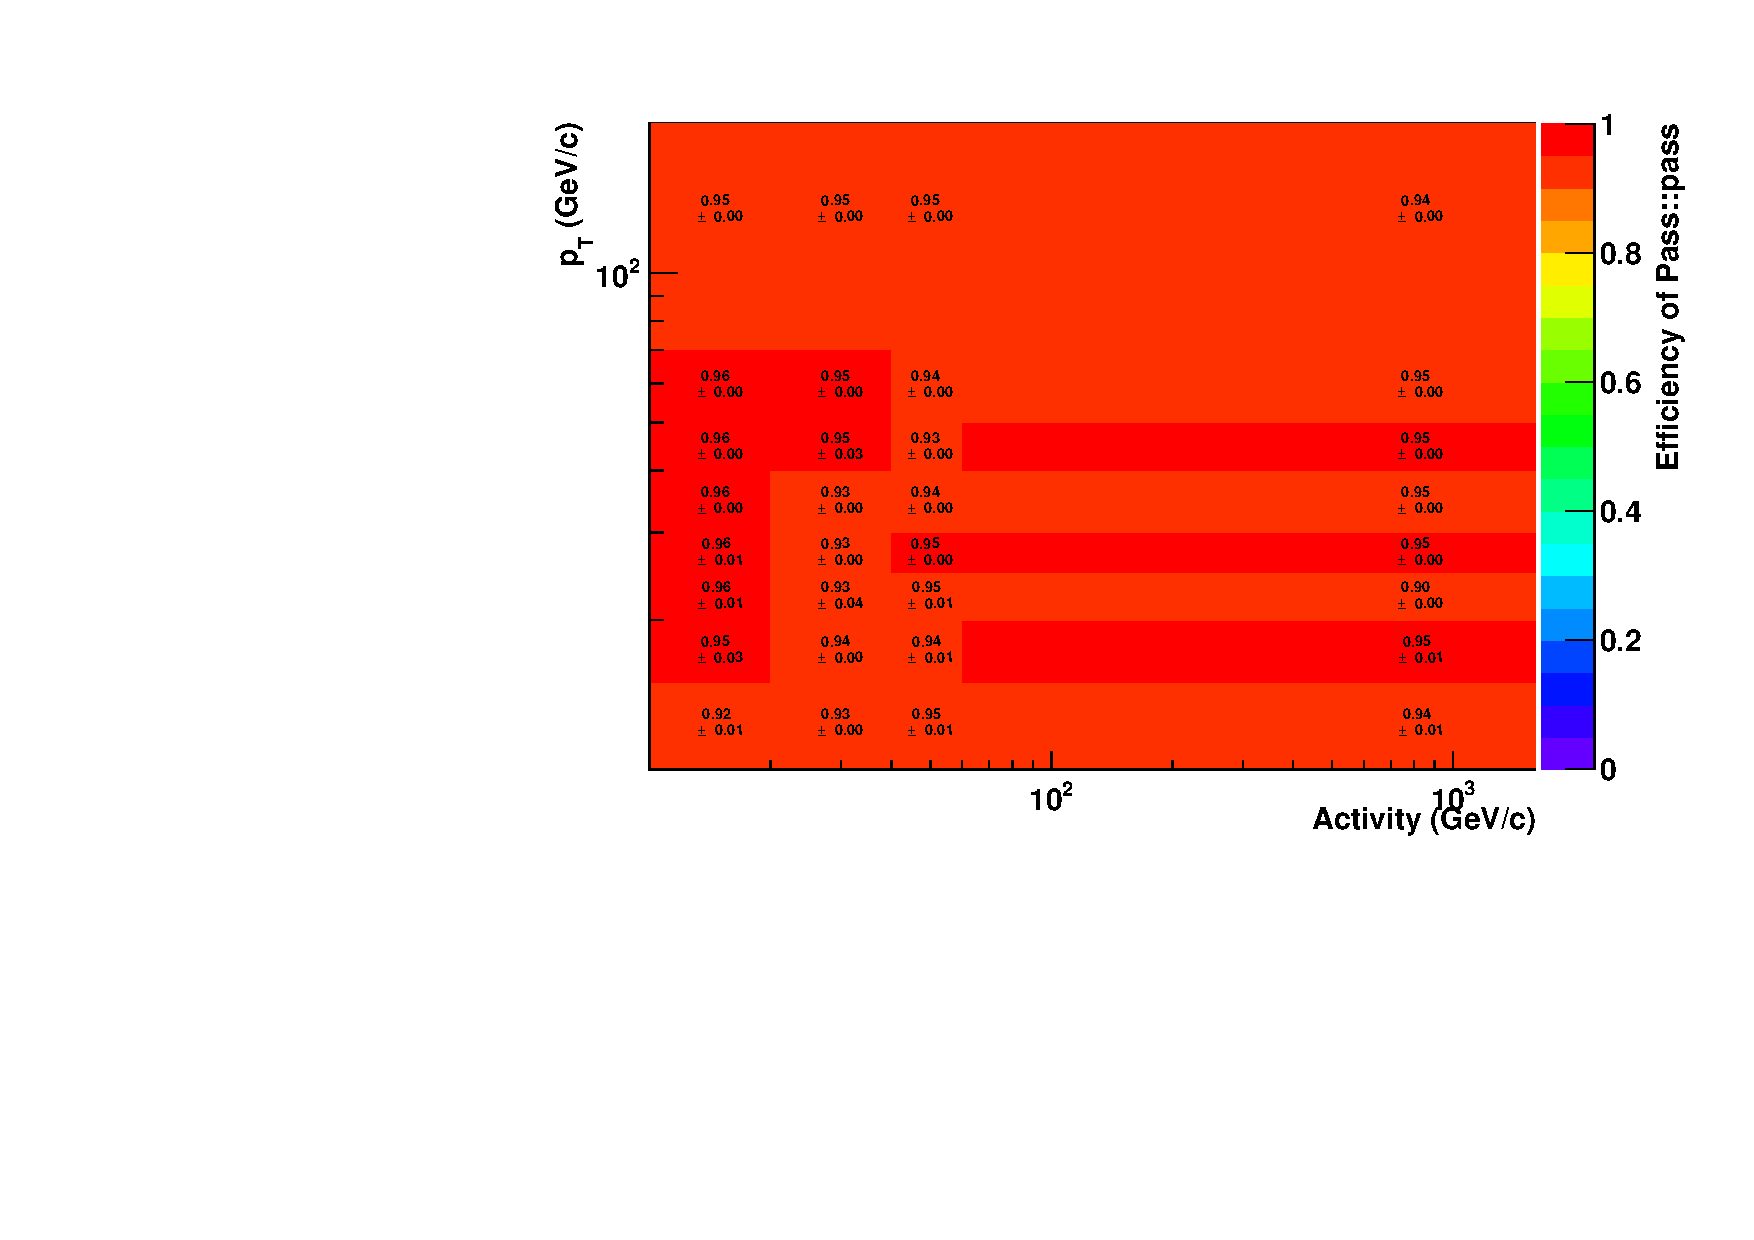
\includegraphics[width=1.\textwidth]{figures/efficiencies/MuRecoTagAndProbePTActivity.pdf}};
    \begin{scope}[x={(image.south east)},y={(image.north west)}]
%         \draw[red,ultra thick,rounded corners] (0.62,0.65) rectangle (0.78,0.75);
%         \draw[red,ultra thick,rounded corners] (0.60,0.01) rectangle (0.75,0.99); % cordinates unten links(x,y) oben rechts(x,y)
    \end{scope}
   \end{tikzpicture}
   \end{column}
  \end{columns}
\begin{itemize}
 \item Tag \& Probe reco efficiencies tend to be higher than \ttbar \& \wpj efficiencies.
 \item Compensating effects at work? Tag \& Probe efficiency are overall lower but to be probed lepton already needs to be reconstructed as muon therefore all lost muons due to not being reconstructed are not tested.

\end{itemize}

\end{frame}


\begin{frame}
 \begin{block}{}
 \centering
 \Large Lost-Lepton ToDo List
 \end{block}


\end{frame}

\subsection{Lost-Lepton Method}
\begin{frame}
 \begin{center}
\begin{tikzpicture}
    \node[anchor=south west,inner sep=0] (image) at (0,0) {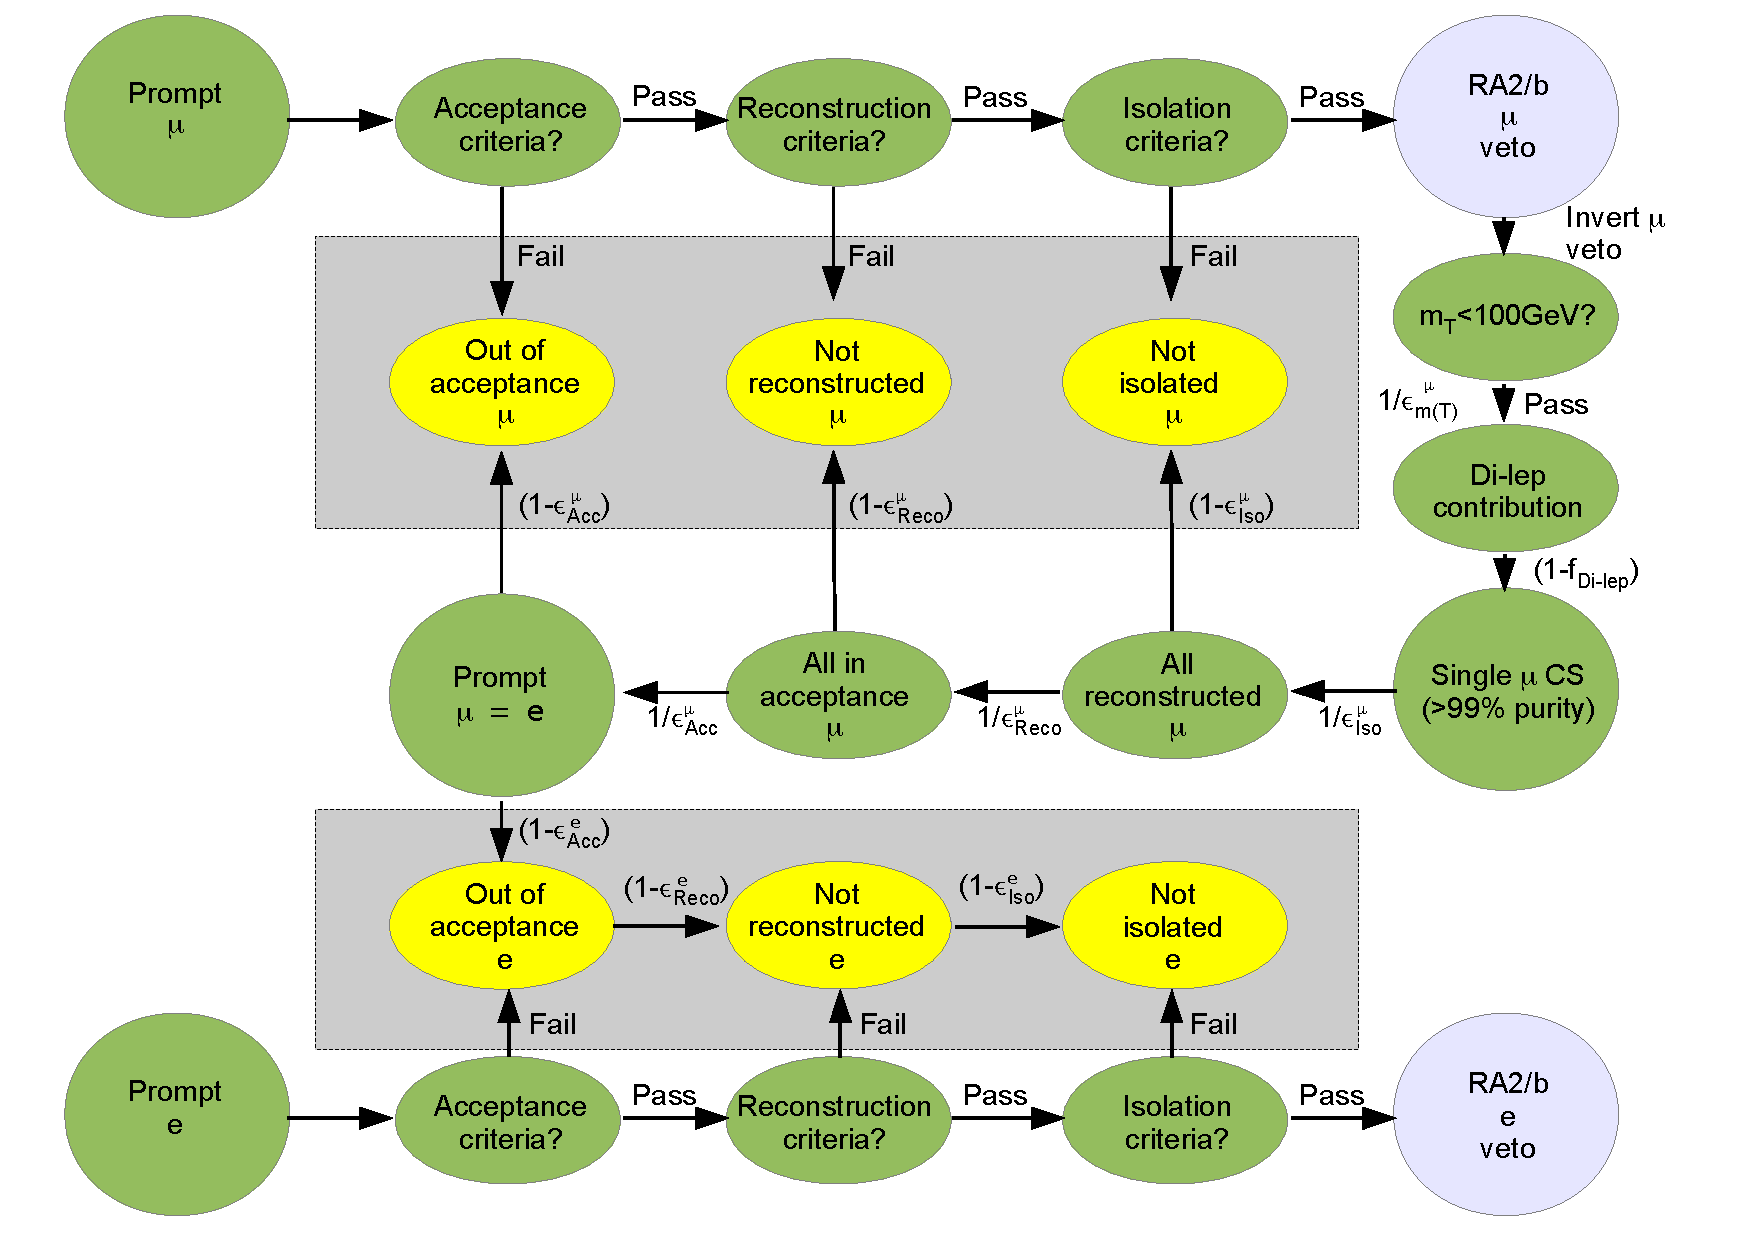
\includegraphics[width=0.75\textwidth]{figures/Sketches/LostLeptonSketch_mu_pred_full.pdf}};
    \begin{scope}[x={(image.south east)},y={(image.north west)}]
%         \draw[red,ultra thick,rounded corners] (0.62,0.65) rectangle (0.78,0.75);
         \draw[yellow,ultra thick,rounded corners] (0.785,0.81) rectangle (0.955,1.01); % cordinates unten links(x,y) oben rechts(x,y)
         \draw[yellow,ultra thick,rounded corners] (0.785,0.01) rectangle (0.955,.21); % cordinates unten links(x,y) oben rechts(x,y)
         \draw[green,ultra thick,rounded corners] (0.785,0.7) rectangle (0.955,0.79); % cordinates unten links(x,y) oben rechts(x,y)
         \draw[green,ultra thick,rounded corners] (0.785,0.555) rectangle (0.955,0.65); % cordinates unten links(x,y) oben rechts(x,y)
         \draw[green,ultra thick,rounded corners] (0.785,0.36) rectangle (0.955,0.51); % cordinates unten links(x,y) oben rechts(x,y)
         \draw[red,ultra thick,rounded corners] (0.60,0.01) rectangle (0.75,0.99); % cordinates unten links(x,y) oben rechts(x,y)
         \draw[blue,ultra thick,rounded corners] (0.40,0.01) rectangle (0.55,0.99); % cordinates unten links(x,y) oben rechts(x,y)
         \draw[black,ultra thick,rounded corners] (0.21,0.01) rectangle (0.365,0.99); % cordinates unten links(x,y) oben rechts(x,y)
    \end{scope}
\end{tikzpicture}

 
 \begin{itemize}
  \item Three major Efficiencies: Acc, Reco, Iso
  \item Three minor Efficiencies: \mt cut, Di-Lep, Purity
  \item Lepton Definition \& Isolated Tracks
 \end{itemize}
 \end{center}
\end{frame}


\begin{frame}
 \frametitle{Status - ToDo}
 \begin{itemize}
  \item Acceptance Efficiencies
  \begin{itemize}
   \item Need to come directly from MC
   \item Best: Take Acceptance Correction for each search bin $\rightarrow$ Specify `Final` search bins
   \item Uncertainty: Statistics of Efficiencies (MC stats) \& PDF uncertainties
  \end{itemize}
  \item Reco, Iso Efficiencies
  \begin{itemize}
   \item Binning and Parametrization optimization (best for final search bins)
   \item Could come from MC (validate using Tag \& Probe)
   \item Best obtain directly from Data (Tag \& Probe)

  \item Tag \& Probe:
 \begin{itemize}
  \item Machinery up and running
  \item First try obtaining ID and Iso efficiencies from \Zll seem to be significant lower
 \end{itemize}
 \end{itemize}
 \item Other Efficiencies:
 \begin{itemize}
  \item Isolated Track Veto: (Merge into lepton definition?)
  \item \mt cut: Derive uncertainty by varying JEC
  \item Di-Lep: Rather low conservative uncertainty of 50\% negligible
  \item Purity of CS Uncertainty from data?
 \end{itemize}

 \end{itemize}

\end{frame}
%%%%%%%%%%%%%%%%%%%%%%%%%%%%%%%%%%%%%%%%%%%%%%%%%%%%%%%%%%%%%%%%%%%%%%%%%%%%%%%5
%%%%%%%%%%%%55
%%%%%%%%%%%%%%%%%%%%%%%55
%%%%%%%%%%%%%%%%%%%%%%%%%%%%%%%%%%%%%%%%%%%%%%%%%%%%%%%%%%%%%%%%%%%%%%%%%%%%%%%5
\begin{frame}
 \begin{block}{}
 \centering
 \Large Backup
 \end{block}
\end{frame}


\subsection{Muon Efficiencies}
\begin{frame}
 \begin{center}
    {\Large Efficiencies: Muon}
  \end{center}
\end{frame}

\begin{frame}
\frametitle{$\mu$ iso}
   \begin{columns}
    \begin{column}{0.33\textwidth}
     \centering
      \begin{overpic}[width=1.00\textwidth]{figures/efficiencies/MuIsoHT1D.pdf}
     \end{overpic}
      \begin{overpic}[width=1.00\textwidth]{figures/efficiencies/MuIsoNJets1D.pdf}
     \end{overpic}
    \end{column}
    \begin{column}{0.33\textwidth}
      \centering
      \begin{overpic}[width=1.00\textwidth]{figures/efficiencies/MuIsoMHT1D.pdf}      \end{overpic}
      \centering
      \begin{overpic}[width=1.00\textwidth]{figures/efficiencies/MuIsoPT.pdf}      \end{overpic}
    \end{column}
    \begin{column}{0.33\textwidth}
     \centering
      \begin{overpic}[width=1.00\textwidth]{figures/efficiencies/MuIsoBTag1D.pdf}      \end{overpic}
      \begin{overpic}[width=1.00\textwidth]{figures/efficiencies/MuIsoActivity.pdf} \end{overpic}

    \end{column}

  \end{columns}
\end{frame}

\begin{frame}
 \frametitle{$\mu$ iso used parametization and binnning}
\centering
      \begin{overpic}[width=0.90\textwidth]{figures/efficiencies/MuIsoPTActivity.pdf}
     \end{overpic}
\end{frame}

\begin{frame}
\frametitle{$\mu$ reco}
   \begin{columns}
    \begin{column}{0.33\textwidth}
     \centering
      \begin{overpic}[width=1.00\textwidth]{figures/efficiencies/MuRecoHT1D.pdf}
     \end{overpic}
      \begin{overpic}[width=1.00\textwidth]{figures/efficiencies/MuRecoNJets1D.pdf}
     \end{overpic}
    \end{column}
    \begin{column}{0.33\textwidth}
      \centering
      \begin{overpic}[width=1.00\textwidth]{figures/efficiencies/MuRecoMHT1D.pdf}      \end{overpic}
      \centering
      \begin{overpic}[width=1.00\textwidth]{figures/efficiencies/MuRecoPT.pdf}      \end{overpic}
    \end{column}
    \begin{column}{0.33\textwidth}
     \centering
      \begin{overpic}[width=1.00\textwidth]{figures/efficiencies/MuRecoBTag1D.pdf}      \end{overpic}
         \begin{overpic}[width=1.00\textwidth]{figures/efficiencies/MuRecoActivity.pdf} \end{overpic}

    \end{column}

  \end{columns}
\end{frame}

\begin{frame}
 \frametitle{$\mu$ reco used parametization and binnning}
\centering
      \begin{overpic}[width=0.90\textwidth]{figures/efficiencies/MuRecoPTActivity.pdf}
     \end{overpic}
\end{frame}

\begin{frame}
\frametitle{$\mu$ acc}
   \begin{columns}
    \begin{column}{0.33\textwidth}
     \centering
      \begin{overpic}[width=1.00\textwidth]{figures/efficiencies/MuAccHT1D.pdf}
     \end{overpic}
      \begin{overpic}[width=1.00\textwidth]{figures/efficiencies/MuAccNJets1D.pdf}
     \end{overpic}
    \end{column}
    \begin{column}{0.33\textwidth}
      \centering
      \begin{overpic}[width=1.00\textwidth]{figures/efficiencies/MuAccMHT1D.pdf}      \end{overpic}
      \begin{overpic}[width=1.00\textwidth]{figures/efficiencies/MuAccActivity.pdf} \end{overpic}
      \centering
    \end{column}
    \begin{column}{0.33\textwidth}
     \centering
      \begin{overpic}[width=1.00\textwidth]{figures/efficiencies/MuAccBTag1D.pdf}      \end{overpic}
\begin{overpic}[width=1.00\textwidth]{figures/efficiencies/MuAccPT.pdf}      \end{overpic}

    \end{column}

  \end{columns}
\end{frame}

\begin{frame}
 \frametitle{$\mu$ acc used parametization and binnning}
\centering
      \begin{overpic}[width=0.90\textwidth]{figures/efficiencies/MuAccBTagNJets.pdf}
     \end{overpic}
\end{frame}

\begin{frame}
\frametitle{$\mu$ Purity}
   \begin{columns}
    \begin{column}{0.33\textwidth}
     \centering
      \begin{overpic}[width=1.00\textwidth]{figures/efficiencies/MuPurityHT1D.pdf}
     \end{overpic}
      \begin{overpic}[width=1.00\textwidth]{figures/efficiencies/MuPurityNJets1D.pdf}
     \end{overpic}
    \end{column}
    \begin{column}{0.33\textwidth}
      \centering
      \begin{overpic}[width=1.00\textwidth]{figures/efficiencies/MuPurityMHT1D.pdf}      \end{overpic}
      \begin{overpic}[width=1.00\textwidth]{figures/efficiencies/MuPurityActivity.pdf} \end{overpic}
      \centering
    \end{column}
    \begin{column}{0.33\textwidth}
     \centering
      \begin{overpic}[width=1.00\textwidth]{figures/efficiencies/MuPurityBTag1D.pdf}      \end{overpic}
\begin{overpic}[width=1.00\textwidth]{figures/efficiencies/MuPurityPT.pdf}      \end{overpic}

    \end{column}

  \end{columns}
\end{frame}


\begin{frame}
 \begin{center}
    {\Large $\mu$ purity not corrected for!}
  \end{center}
\end{frame}

\begin{frame}
\frametitle{$\mu$ \mt-cut}
   \begin{columns}
    \begin{column}{0.33\textwidth}
     \centering
      \begin{overpic}[width=1.00\textwidth]{figures/efficiencies/MuMTWHT1D.pdf}
     \end{overpic}
      \begin{overpic}[width=1.00\textwidth]{figures/efficiencies/MuMTWNJets1D.pdf}
     \end{overpic}
    \end{column}
    \begin{column}{0.33\textwidth}
      \centering
      \begin{overpic}[width=1.00\textwidth]{figures/efficiencies/MuMTWMHT1D.pdf}      \end{overpic}
      \begin{overpic}[width=1.00\textwidth]{figures/efficiencies/MuMTWActivity.pdf} \end{overpic}
      \centering
    \end{column}
    \begin{column}{0.33\textwidth}
     \centering
      \begin{overpic}[width=1.00\textwidth]{figures/efficiencies/MuMTWBTag1D.pdf}      \end{overpic}
\begin{overpic}[width=1.00\textwidth]{figures/efficiencies/MuMTWPT.pdf}      \end{overpic}

    \end{column}

  \end{columns}
\end{frame}


\begin{frame}
 \frametitle{$\mu$ \mt-cut used parametization and binnning}
\centering
      \begin{overpic}[width=0.90\textwidth]{figures/efficiencies/MuMTWPTActivity.pdf}
     \end{overpic}
\end{frame}


\begin{frame}
\frametitle{$\mu$ di lep contribution to control sample}
   \begin{columns}
    \begin{column}{0.33\textwidth}
     \centering
      \begin{overpic}[width=1.00\textwidth]{figures/efficiencies/MuDiLepContributionMTWHT1D.pdf}
     \end{overpic}
      \begin{overpic}[width=1.00\textwidth]{figures/efficiencies/MuDiLepContributionMTWNJets1D.pdf}
     \end{overpic}
    \end{column}
    \begin{column}{0.33\textwidth}
      \centering
      \begin{overpic}[width=1.00\textwidth]{figures/efficiencies/MuDiLepContributionMTWMHT1D.pdf}      \end{overpic}
            \begin{overpic}[width=1.00\textwidth]{figures/efficiencies/MuDiLepContributionMTWBTag1D.pdf}      \end{overpic}
      \centering
    \end{column}
  \end{columns}
\end{frame}


\begin{frame}
 \frametitle{$\mu$ di lep contamination used parametization and binnning}
\centering
      \begin{overpic}[width=1.00\textwidth]{figures/efficiencies/MuDiLepContributionMTWNJets1D.pdf}
     \end{overpic}
\end{frame}
\begin{frame}
\frametitle{Di-lep efficieny (amount of lost di-leptonic decays)}
   \begin{columns}
    \begin{column}{0.33\textwidth}
     \centering
      \begin{overpic}[width=1.00\textwidth]{figures/efficiencies/MuDiLepMTWHT1D.pdf}
     \end{overpic}
      \begin{overpic}[width=1.00\textwidth]{figures/efficiencies/MuDiLepMTWNJets1D.pdf}
     \end{overpic}
    \end{column}
    \begin{column}{0.33\textwidth}
      \centering
      \begin{overpic}[width=1.00\textwidth]{figures/efficiencies/MuDiLepMTWMHT1D.pdf}      \end{overpic}
            \begin{overpic}[width=1.00\textwidth]{figures/efficiencies/MuDiLepMTWBTag1D.pdf}      \end{overpic}
      \centering
    \end{column}
  \end{columns}
\end{frame}


\begin{frame}
 \frametitle{Di-lep efficieny (amount of lost di-leptonic decays) used parametization and binnning}
\centering
      \begin{overpic}[width=1.00\textwidth]{figures/efficiencies/MuDiLepMTWNJets1D.pdf}
     \end{overpic}
\end{frame}


\subsection{Electron Efficiencies}
\begin{frame}
 \begin{center}
    {\Large Efficiencies: Electron}
  \end{center}
\end{frame}

\begin{frame}
\frametitle{e iso}
   \begin{columns}
    \begin{column}{0.33\textwidth}
     \centering
      \begin{overpic}[width=1.00\textwidth]{figures/efficiencies/ElecIsoHT1D.pdf}
     \end{overpic}
      \begin{overpic}[width=1.00\textwidth]{figures/efficiencies/ElecIsoNJets1D.pdf}
     \end{overpic}
    \end{column}
    \begin{column}{0.33\textwidth}
      \centering
      \begin{overpic}[width=1.00\textwidth]{figures/efficiencies/ElecIsoMHT1D.pdf}      \end{overpic}
      \centering
      \begin{overpic}[width=1.00\textwidth]{figures/efficiencies/ElecIsoPT.pdf}      \end{overpic}
    \end{column}
    \begin{column}{0.33\textwidth}
     \centering
      \begin{overpic}[width=1.00\textwidth]{figures/efficiencies/ElecIsoBTag1D.pdf}      \end{overpic}
      \begin{overpic}[width=1.00\textwidth]{figures/efficiencies/ElecIsoActivity.pdf} \end{overpic}

    \end{column}

  \end{columns}
\end{frame}

\begin{frame}
 \frametitle{e iso used parametization and binnning}
\centering
      \begin{overpic}[width=0.90\textwidth]{figures/efficiencies/ElecIsoPTActivity.pdf}
     \end{overpic}
\end{frame}

\begin{frame}
\frametitle{e reco}
   \begin{columns}
    \begin{column}{0.33\textwidth}
     \centering
      \begin{overpic}[width=1.00\textwidth]{figures/efficiencies/ElecRecoHT1D.pdf}
     \end{overpic}
      \begin{overpic}[width=1.00\textwidth]{figures/efficiencies/ElecRecoNJets1D.pdf}
     \end{overpic}
    \end{column}
    \begin{column}{0.33\textwidth}
      \centering
      \begin{overpic}[width=1.00\textwidth]{figures/efficiencies/ElecRecoMHT1D.pdf}      \end{overpic}
      \centering
      \begin{overpic}[width=1.00\textwidth]{figures/efficiencies/ElecRecoPT.pdf}      \end{overpic}
    \end{column}
    \begin{column}{0.33\textwidth}
     \centering
      \begin{overpic}[width=1.00\textwidth]{figures/efficiencies/ElecRecoBTag1D.pdf}      \end{overpic}
         \begin{overpic}[width=1.00\textwidth]{figures/efficiencies/ElecRecoActivity.pdf} \end{overpic}

    \end{column}

  \end{columns}
\end{frame}


\begin{frame}
 \frametitle{e reco used parametization and binnning}
\centering
      \begin{overpic}[width=0.90\textwidth]{figures/efficiencies/ElecRecoPTActivity.pdf}
     \end{overpic}
\end{frame}


\begin{frame}
\frametitle{e acc}
   \begin{columns}
    \begin{column}{0.33\textwidth}
     \centering
      \begin{overpic}[width=1.00\textwidth]{figures/efficiencies/ElecAccHT1D.pdf}
     \end{overpic}
      \begin{overpic}[width=1.00\textwidth]{figures/efficiencies/ElecAccNJets1D.pdf}
     \end{overpic}
    \end{column}
    \begin{column}{0.33\textwidth}
      \centering
      \begin{overpic}[width=1.00\textwidth]{figures/efficiencies/ElecAccMHT1D.pdf}      \end{overpic}
      \begin{overpic}[width=1.00\textwidth]{figures/efficiencies/ElecAccActivity.pdf} \end{overpic}
      \centering
    \end{column}
    \begin{column}{0.33\textwidth}
     \centering
      \begin{overpic}[width=1.00\textwidth]{figures/efficiencies/ElecAccBTag1D.pdf}      \end{overpic}
\begin{overpic}[width=1.00\textwidth]{figures/efficiencies/ElecAccPT.pdf}      \end{overpic}

    \end{column}

  \end{columns}
\end{frame}

\begin{frame}
 \frametitle{e acc used parametization and binnning}
\centering
      \begin{overpic}[width=0.90\textwidth]{figures/efficiencies/ElecAccBTagNJets.pdf}
     \end{overpic}
\end{frame}

\begin{frame}
\frametitle{e Purity}
   \begin{columns}
    \begin{column}{0.33\textwidth}
     \centering
      \begin{overpic}[width=1.00\textwidth]{figures/efficiencies/ElecPurityHT1D.pdf}
     \end{overpic}
      \begin{overpic}[width=1.00\textwidth]{figures/efficiencies/ElecPurityNJets1D.pdf}
     \end{overpic}
    \end{column}
    \begin{column}{0.33\textwidth}
      \centering
      \begin{overpic}[width=1.00\textwidth]{figures/efficiencies/ElecPurityMHT1D.pdf}      \end{overpic}
      \begin{overpic}[width=1.00\textwidth]{figures/efficiencies/ElecPurityActivity.pdf} \end{overpic}
      \centering
    \end{column}
    \begin{column}{0.33\textwidth}
     \centering
      \begin{overpic}[width=1.00\textwidth]{figures/efficiencies/ElecPurityBTag1D.pdf}      \end{overpic}
\begin{overpic}[width=1.00\textwidth]{figures/efficiencies/ElecPurityPT.pdf}      \end{overpic}

    \end{column}

  \end{columns}
\end{frame}


\begin{frame}
 \frametitle{e purity used parametization and binnning}
\centering
      \begin{overpic}[width=0.90\textwidth]{figures/efficiencies/ElecPurity.pdf}
     \end{overpic}
\end{frame}

\begin{frame}
\frametitle{e \mt-cut}
   \begin{columns}
    \begin{column}{0.33\textwidth}
     \centering
      \begin{overpic}[width=1.00\textwidth]{figures/efficiencies/ElecMTWHT1D.pdf}
     \end{overpic}
      \begin{overpic}[width=1.00\textwidth]{figures/efficiencies/ElecMTWNJets1D.pdf}
     \end{overpic}
    \end{column}
    \begin{column}{0.33\textwidth}
      \centering
      \begin{overpic}[width=1.00\textwidth]{figures/efficiencies/ElecMTWMHT1D.pdf}      \end{overpic}
      \begin{overpic}[width=1.00\textwidth]{figures/efficiencies/ElecMTWActivity.pdf} \end{overpic}
      \centering
    \end{column}
    \begin{column}{0.33\textwidth}
     \centering
      \begin{overpic}[width=1.00\textwidth]{figures/efficiencies/ElecMTWBTag1D.pdf}      \end{overpic}
\begin{overpic}[width=1.00\textwidth]{figures/efficiencies/ElecMTWPT.pdf}      \end{overpic}

    \end{column}

  \end{columns}
\end{frame}


\begin{frame}
 \frametitle{e \mt-cut used parametization and binnning}
\centering
      \begin{overpic}[width=0.90\textwidth]{figures/efficiencies/ElecMTWPTActivity.pdf}
     \end{overpic}
\end{frame}


\begin{frame}
\frametitle{e di lep contribution to control sample}
   \begin{columns}
    \begin{column}{0.33\textwidth}
     \centering
      \begin{overpic}[width=1.00\textwidth]{figures/efficiencies/ElecDiLepContributionMTWHT1D.pdf}
     \end{overpic}
      \begin{overpic}[width=1.00\textwidth]{figures/efficiencies/ElecDiLepContributionMTWNJets1D.pdf}
     \end{overpic}
    \end{column}
    \begin{column}{0.33\textwidth}
      \centering
      \begin{overpic}[width=1.00\textwidth]{figures/efficiencies/ElecDiLepContributionMTWMHT1D.pdf}      \end{overpic}
            \begin{overpic}[width=1.00\textwidth]{figures/efficiencies/ElecDiLepContributionMTWBTag1D.pdf}      \end{overpic}
      \centering
    \end{column}
  \end{columns}
\end{frame}


\begin{frame}
 \frametitle{e di lep contribution used parametization and binnning}
\centering
      \begin{overpic}[width=1.00\textwidth]{figures/efficiencies/ElecDiLepContributionMTWNJets1D.pdf}
     \end{overpic}
\end{frame}

\begin{frame}
\frametitle{Di-lep efficieny (amount of lost di-leptonic decays)}
   \begin{columns}
    \begin{column}{0.33\textwidth}
     \centering
      \begin{overpic}[width=1.00\textwidth]{figures/efficiencies/MuDiLepMTWHT1D.pdf}
     \end{overpic}
      \begin{overpic}[width=1.00\textwidth]{figures/efficiencies/MuDiLepMTWNJets1D.pdf}
     \end{overpic}
    \end{column}
    \begin{column}{0.33\textwidth}
      \centering
      \begin{overpic}[width=1.00\textwidth]{figures/efficiencies/MuDiLepMTWMHT1D.pdf}      \end{overpic}
            \begin{overpic}[width=1.00\textwidth]{figures/efficiencies/MuDiLepMTWBTag1D.pdf}      \end{overpic}
      \centering
    \end{column}
  \end{columns}
\end{frame}


\begin{frame}
 \frametitle{Di-lep efficieny (amount of lost di-leptonic decays) used parametization and binnning}
\centering
      \begin{overpic}[width=1.00\textwidth]{figures/efficiencies/ElecDiLepContributionMTWNJets1D.pdf}
     \end{overpic}
\end{frame}

\begin{frame}
 \frametitle{Comparison \ttbar \& \wpj vs Tag \& Probe Efficiencies}
  \begin{columns}

   \begin{column}{0.33\textwidth}
     \begin{itemize}
   \item e Iso \ttbar \& \wpj eff. (truth info.)
  \end{itemize}
    \begin{tikzpicture}
    \node[anchor=south west,inner sep=0] (image) at (0,0) {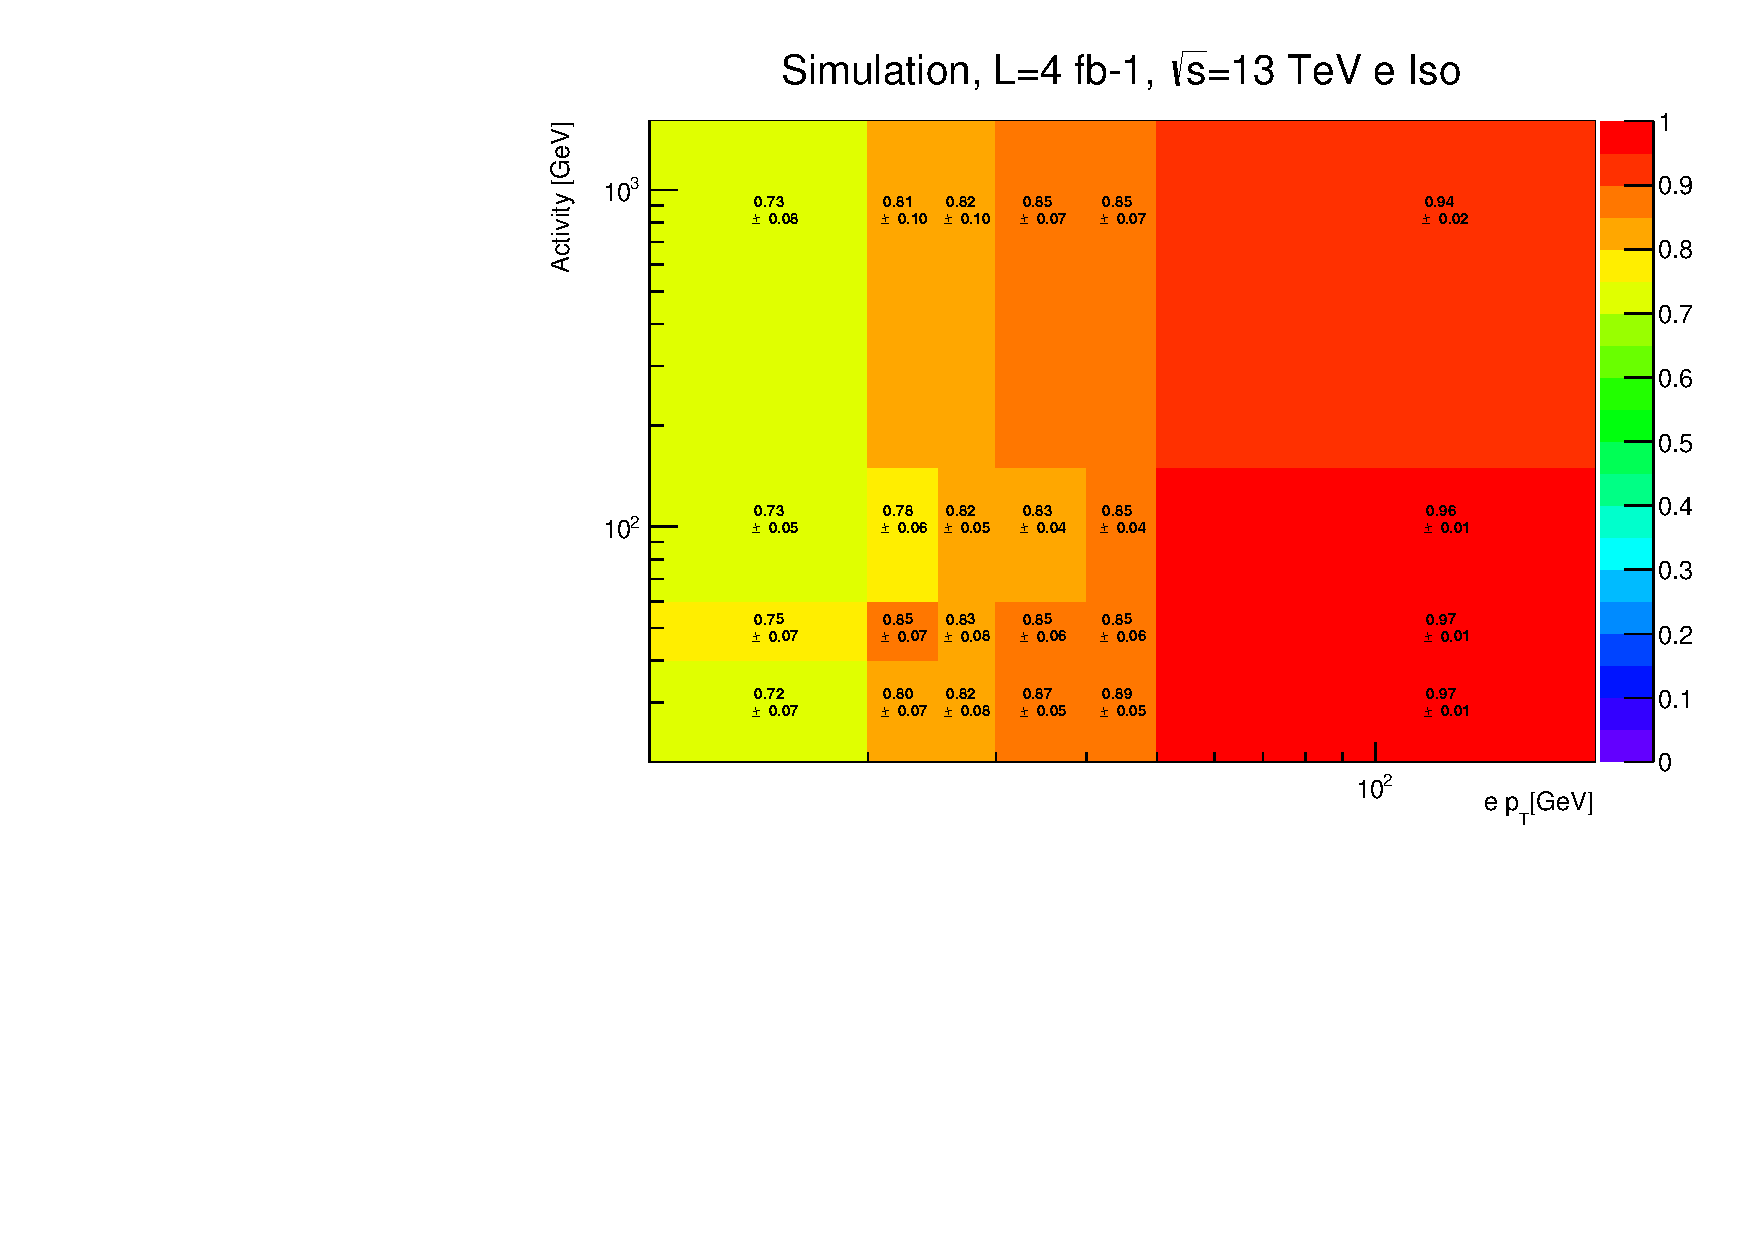
\includegraphics[width=1.\textwidth]{figures/efficiencies/ElecIsoPTActivity_ttbarWPJ.pdf}};
    \begin{scope}[x={(image.south east)},y={(image.north west)}]
%         \draw[red,ultra thick,rounded corners] (0.62,0.65) rectangle (0.78,0.75);
%         \draw[red,ultra thick,rounded corners] (0.60,0.01) rectangle (0.75,0.99); % cordinates unten links(x,y) oben rechts(x,y)
    \end{scope}
   \end{tikzpicture}
   \end{column}
   \begin{column}{0.33\textwidth}
   \begin{itemize}
    \item e Iso DY eff.\\ (truth info.)
   \end{itemize}

    \begin{tikzpicture}
     \node[anchor=south west,inner sep=0] (image) at (0,0) {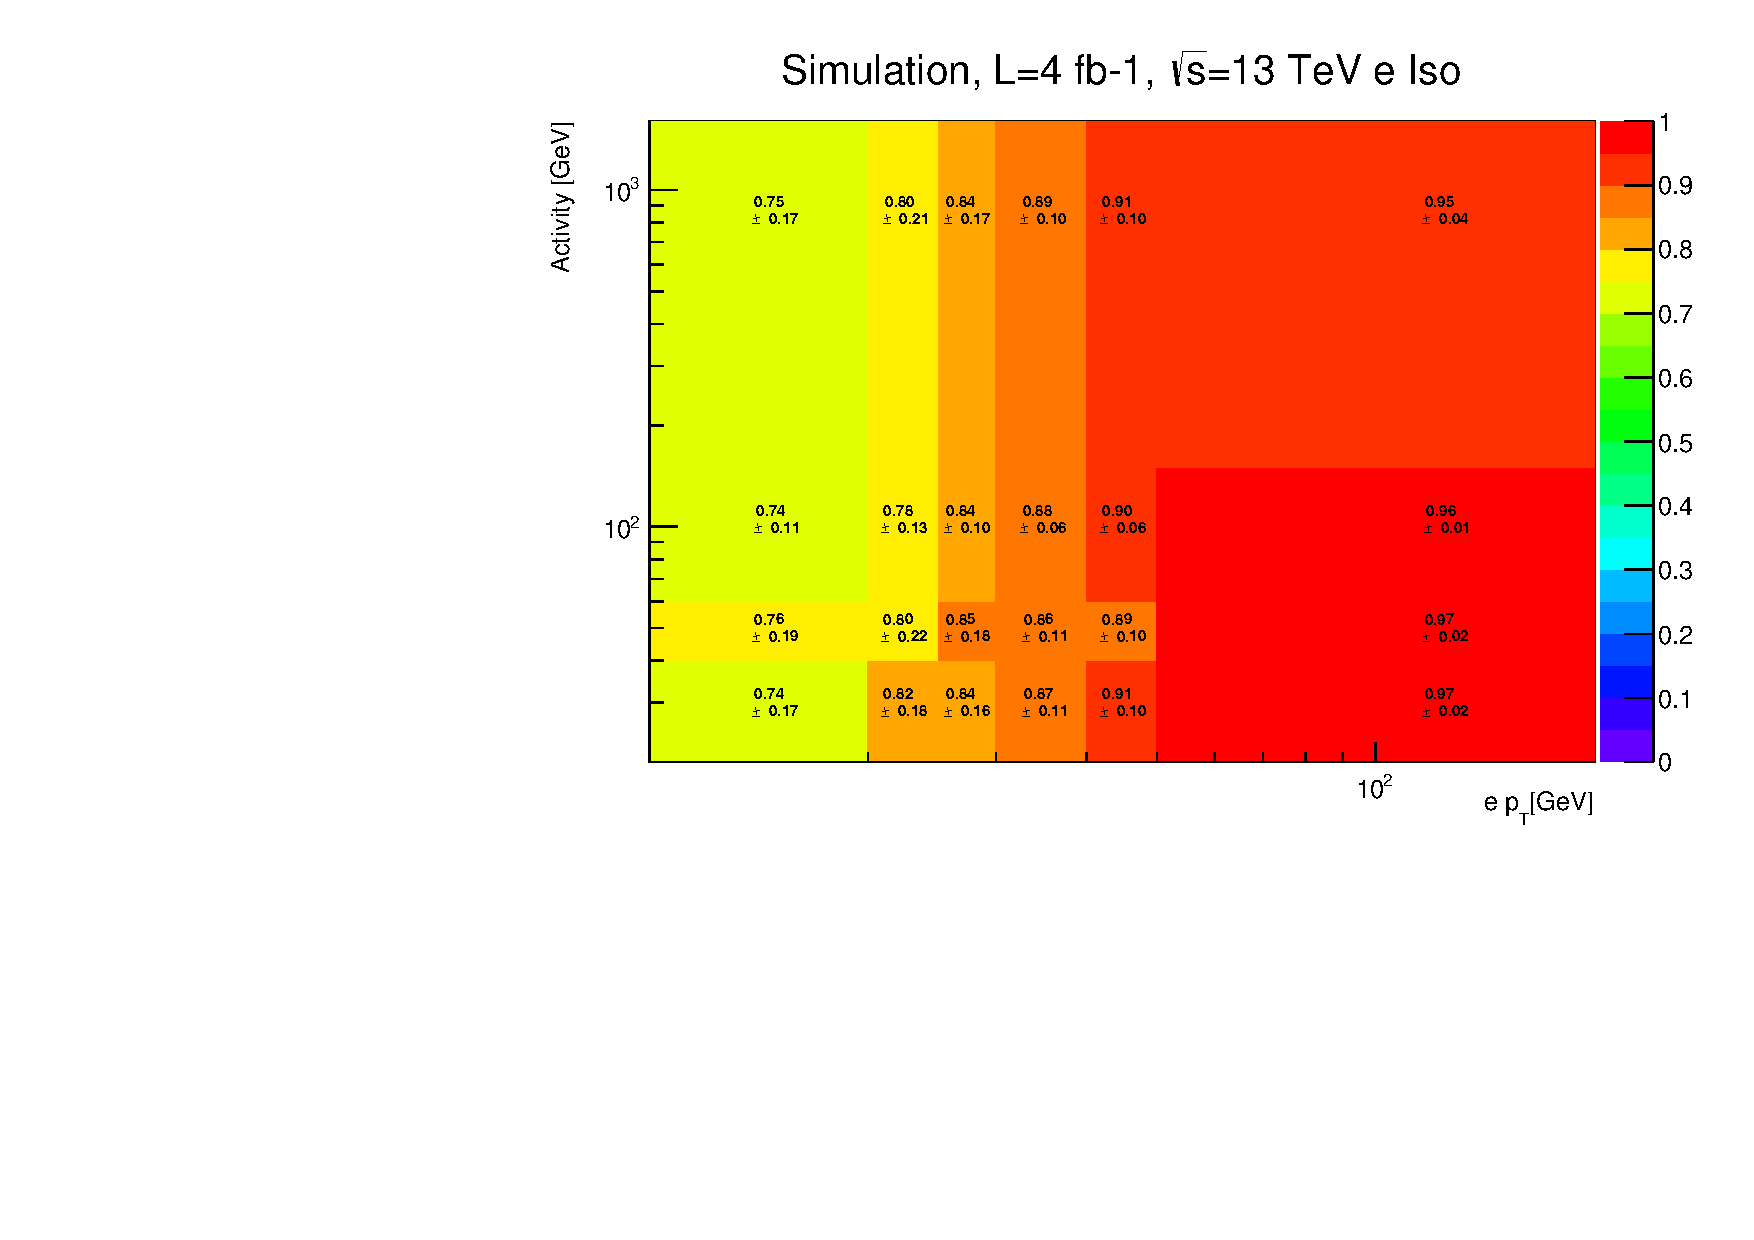
\includegraphics[width=1.\textwidth]{figures/efficiencies/ElecIsoPTActivity_DY_noTagAndProbe.pdf}};
    \begin{scope}[x={(image.south east)},y={(image.north west)}]
%         \draw[red,ultra thick,rounded corners] (0.62,0.65) rectangle (0.78,0.75);
%         \draw[red,ultra thick,rounded corners] (0.60,0.01) rectangle (0.75,0.99); % cordinates unten links(x,y) oben rechts(x,y)
    \end{scope}
   \end{tikzpicture}
   \end{column}
     \begin{column}{0.33\textwidth}
   \begin{itemize}
    \item e Iso Tag \& Probe eff.
   \end{itemize}

    \begin{tikzpicture}
     \node[anchor=south west,inner sep=0] (image) at (0,0) {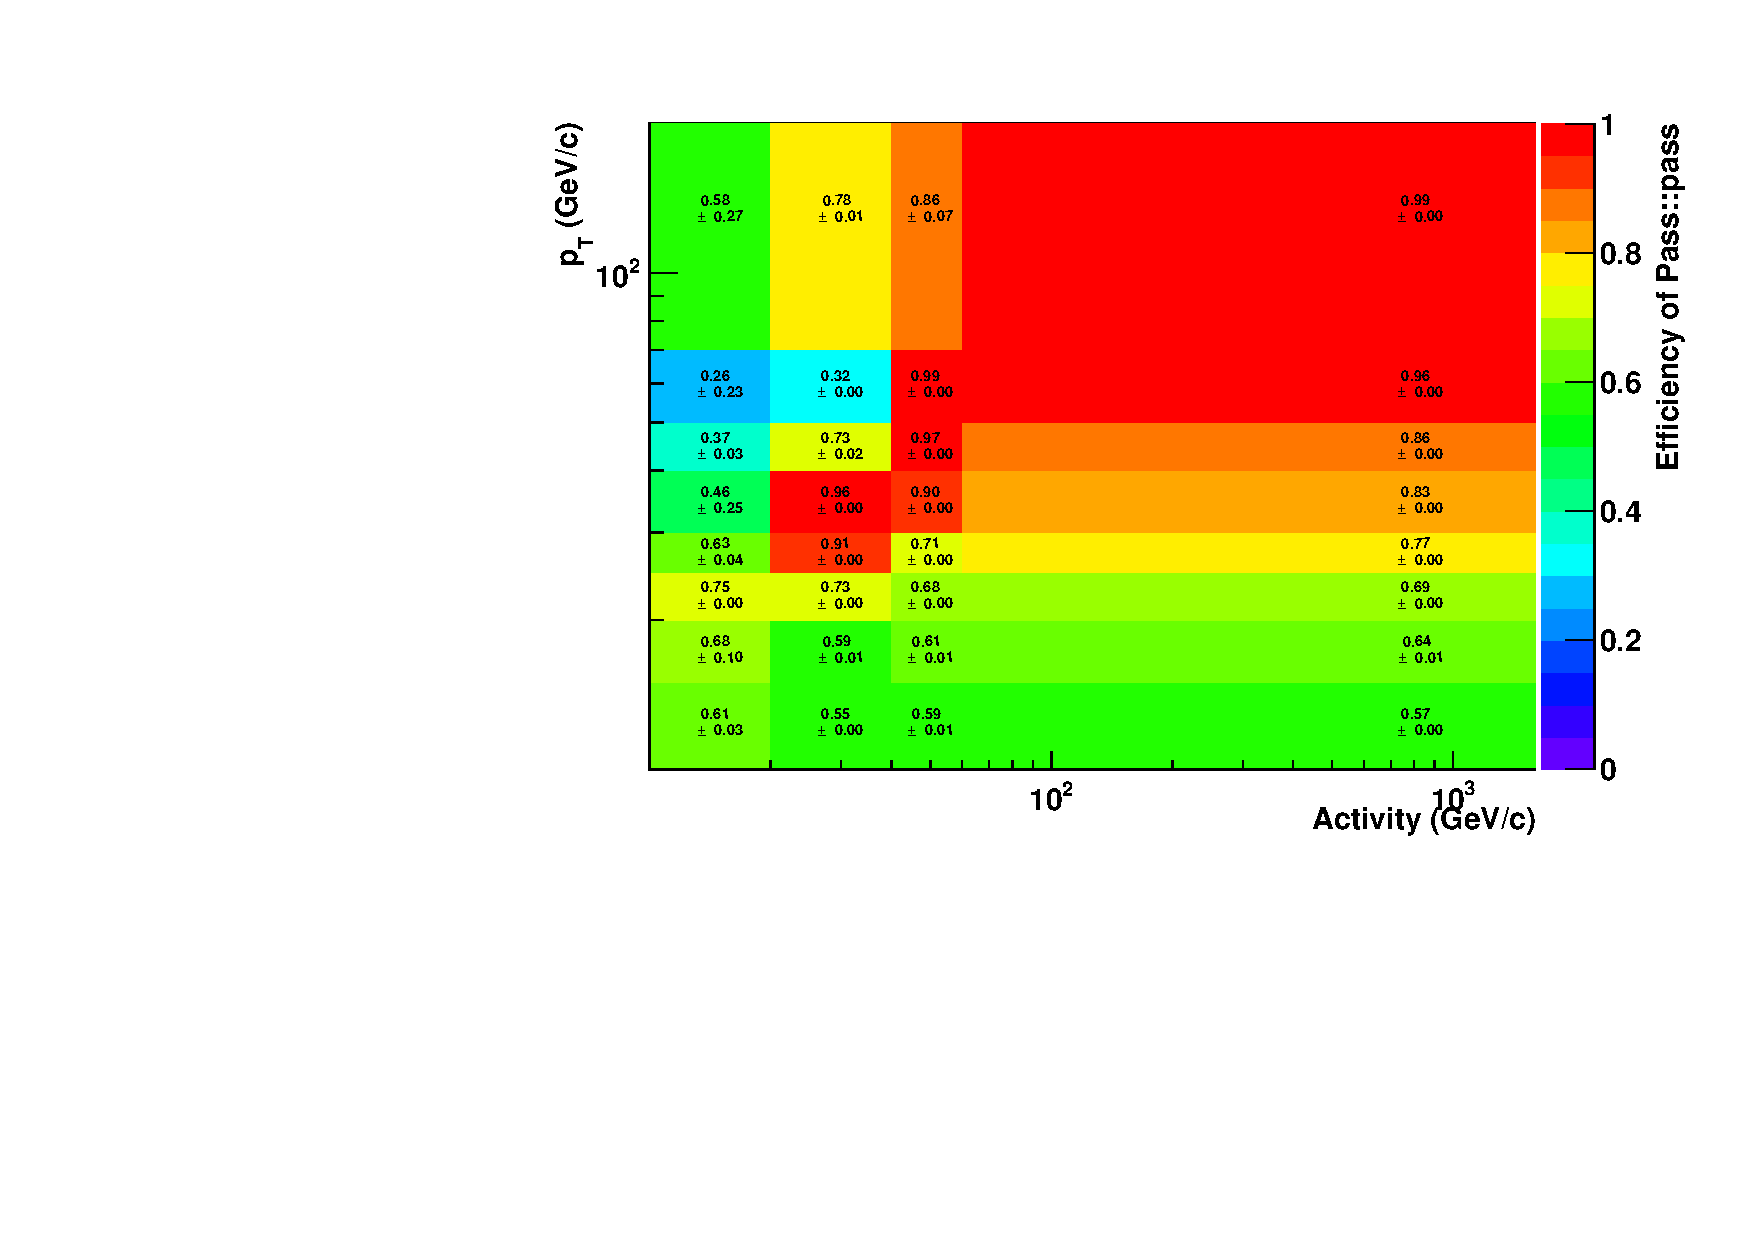
\includegraphics[width=1.\textwidth]{figures/efficiencies/ElecIsoTagAndProbePTActivity.pdf}};
    \begin{scope}[x={(image.south east)},y={(image.north west)}]
%         \draw[red,ultra thick,rounded corners] (0.62,0.65) rectangle (0.78,0.75);
%         \draw[red,ultra thick,rounded corners] (0.60,0.01) rectangle (0.75,0.99); % cordinates unten links(x,y) oben rechts(x,y)
    \end{scope}
   \end{tikzpicture}
   \end{column}
  \end{columns}

\end{frame}

\begin{frame}
 \frametitle{Comparison \ttbar \& \wpj vs Tag \& Probe Efficiencies}
  \begin{columns}

   \begin{column}{0.33\textwidth}
     \begin{itemize}
   \item e ID \ttbar \& \wpj eff. (truth info.)
  \end{itemize}
    \begin{tikzpicture}
    \node[anchor=south west,inner sep=0] (image) at (0,0) {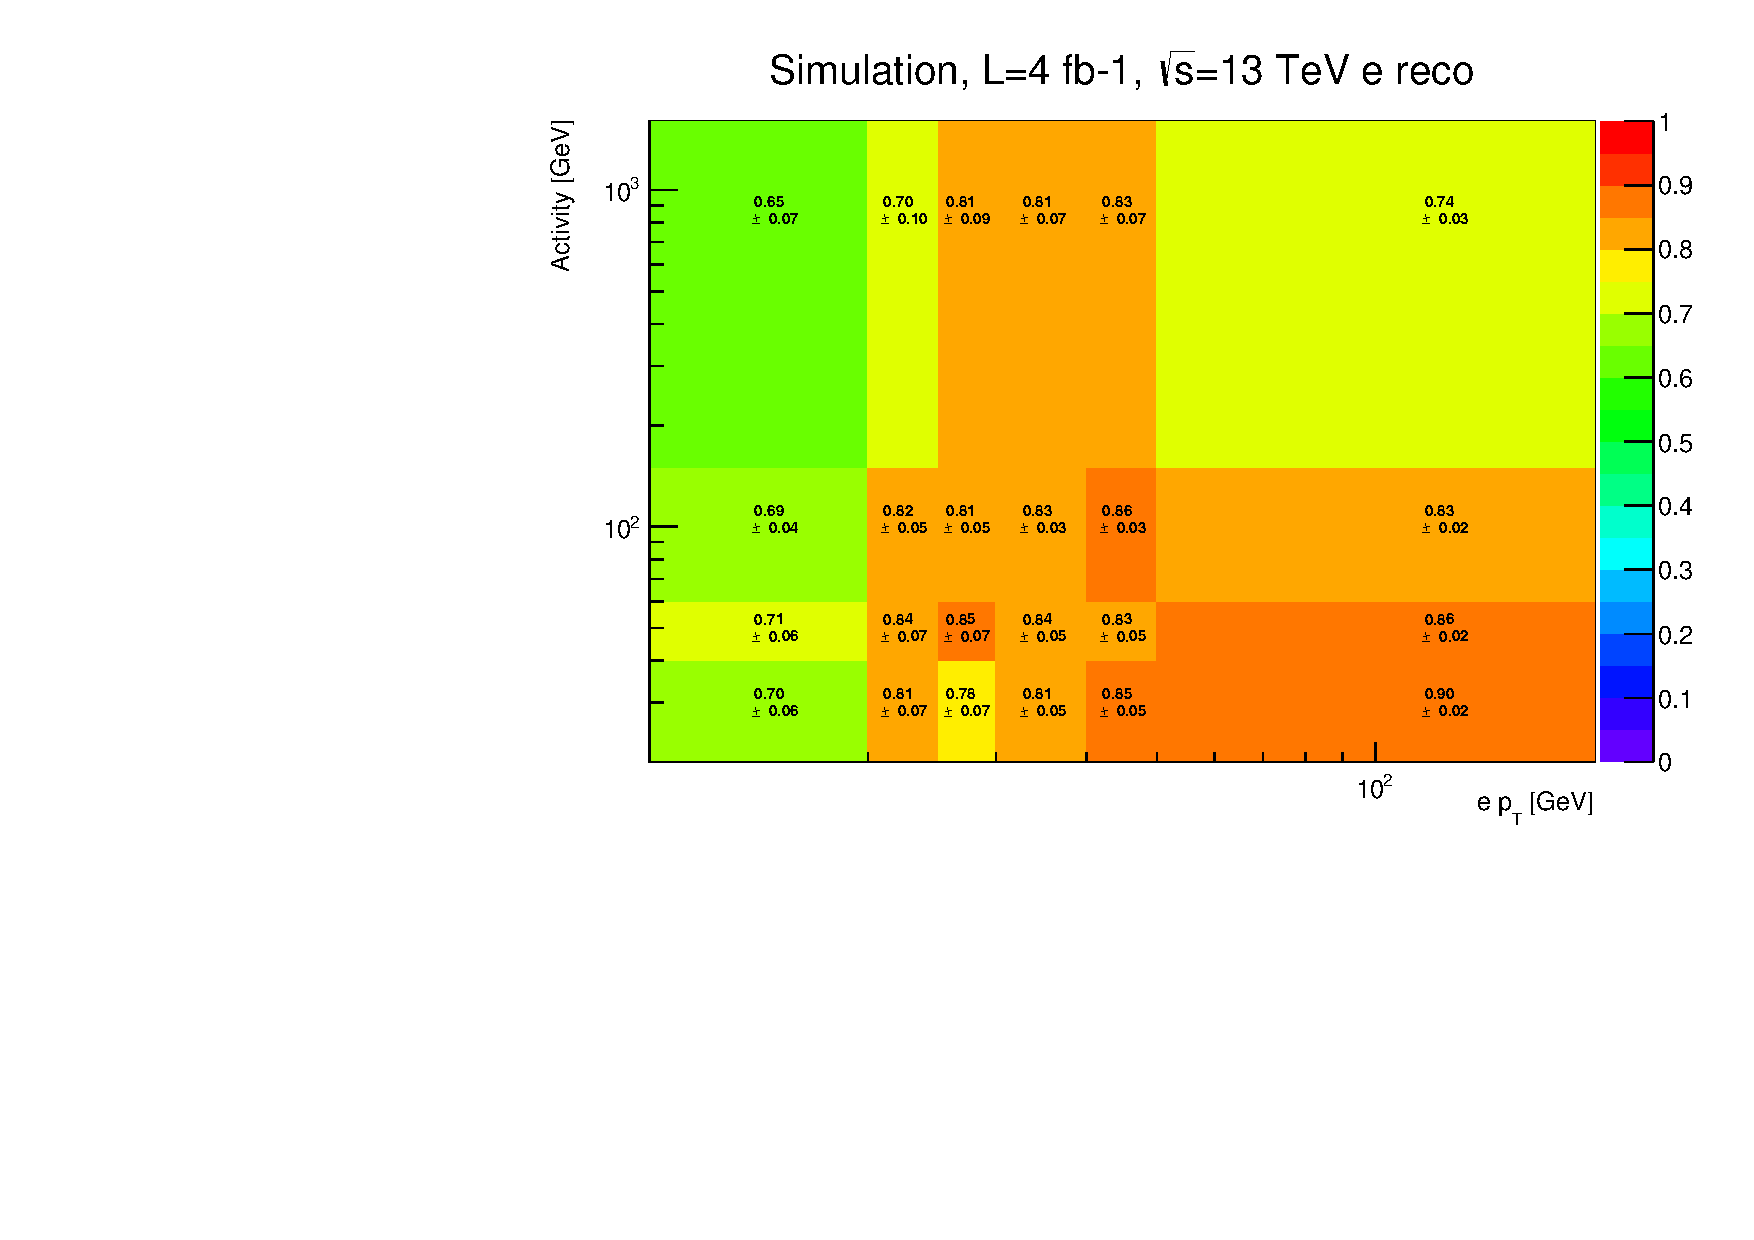
\includegraphics[width=1.\textwidth]{figures/efficiencies/ElecRecoPTActivity_ttbarWPJ.pdf}};
    \begin{scope}[x={(image.south east)},y={(image.north west)}]
%         \draw[red,ultra thick,rounded corners] (0.62,0.65) rectangle (0.78,0.75);
%         \draw[red,ultra thick,rounded corners] (0.60,0.01) rectangle (0.75,0.99); % cordinates unten links(x,y) oben rechts(x,y)
    \end{scope}
   \end{tikzpicture}
   \end{column}
   \begin{column}{0.33\textwidth}
   \begin{itemize}
    \item e ID DY eff.\\ (truth info.)
   \end{itemize}

    \begin{tikzpicture}
     \node[anchor=south west,inner sep=0] (image) at (0,0) {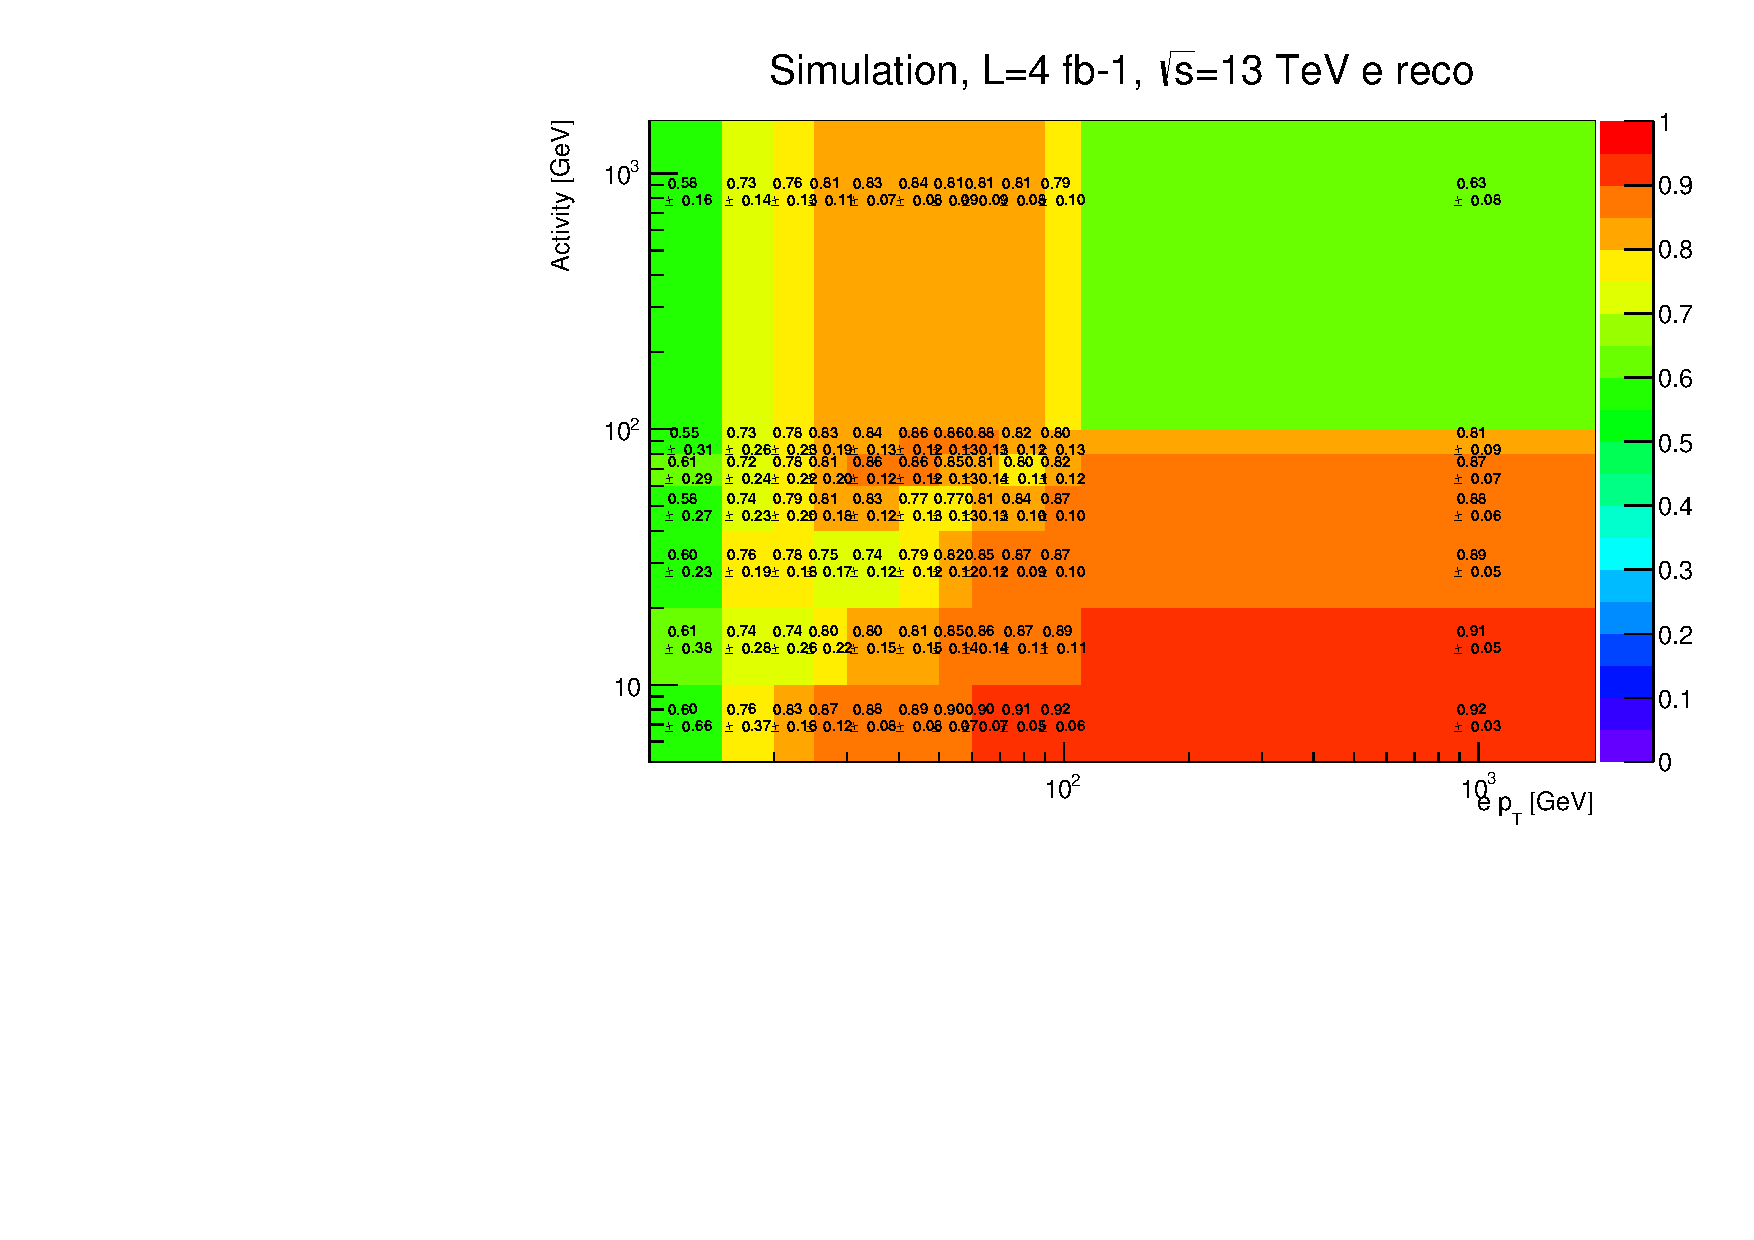
\includegraphics[width=1.\textwidth]{figures/efficiencies/ElecRecoPTActivity_DY_noTagAndProbe.pdf}};
    \begin{scope}[x={(image.south east)},y={(image.north west)}]
%         \draw[red,ultra thick,rounded corners] (0.62,0.65) rectangle (0.78,0.75);
%         \draw[red,ultra thick,rounded corners] (0.60,0.01) rectangle (0.75,0.99); % cordinates unten links(x,y) oben rechts(x,y)
    \end{scope}
   \end{tikzpicture}
   \end{column}
        \begin{column}{0.33\textwidth}
   \begin{itemize}
    \item e Iso Tag \& Probe eff.
   \end{itemize}

    \begin{tikzpicture}
     \node[anchor=south west,inner sep=0] (image) at (0,0) {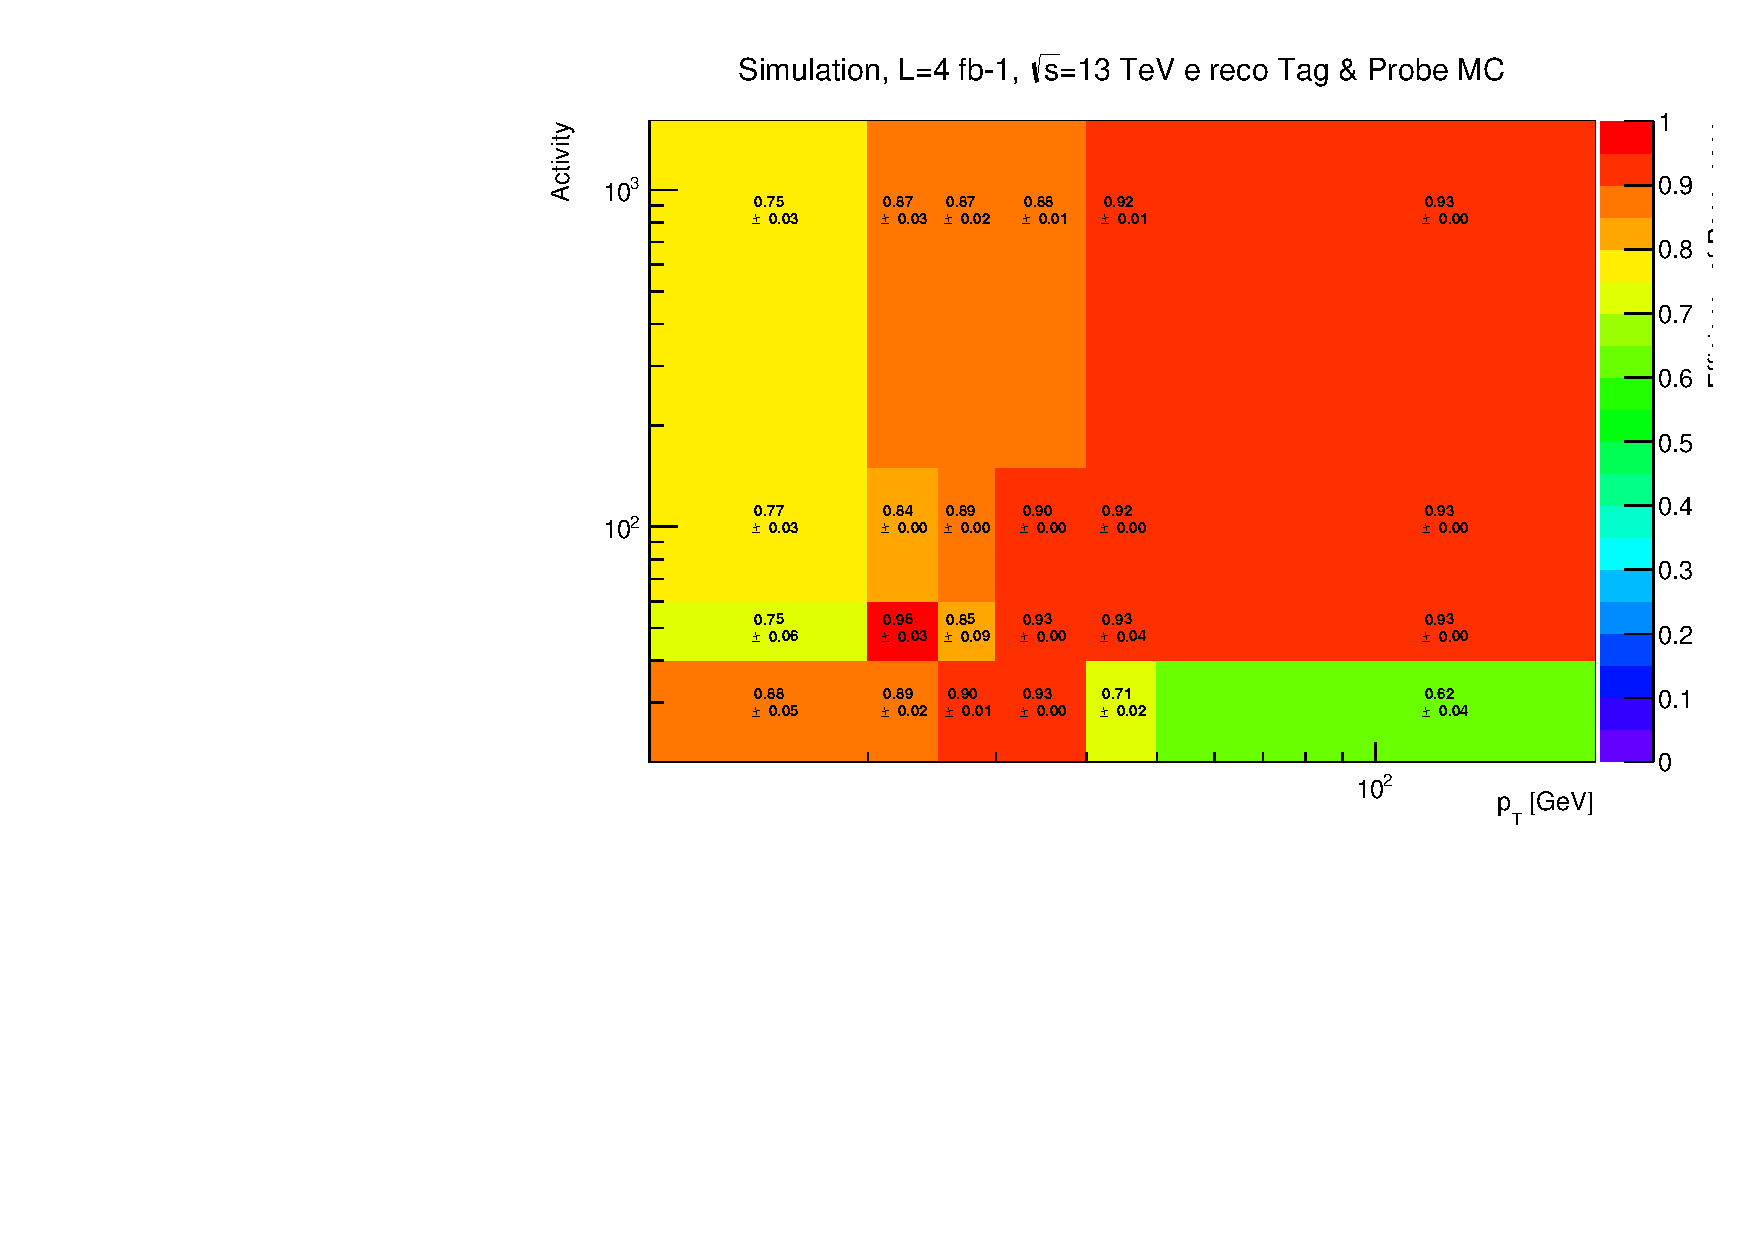
\includegraphics[width=1.\textwidth]{figures/efficiencies/ElecRecoTagAndProbePTActivity.pdf}};
    \begin{scope}[x={(image.south east)},y={(image.north west)}]
%         \draw[red,ultra thick,rounded corners] (0.62,0.65) rectangle (0.78,0.75);
%         \draw[red,ultra thick,rounded corners] (0.60,0.01) rectangle (0.75,0.99); % cordinates unten links(x,y) oben rechts(x,y)
    \end{scope}
   \end{tikzpicture}
   \end{column}
  \end{columns}

\end{frame}

\subsection{Closure Search bins}
\begin{frame}
 \begin{center}
    {\Large Closure for fine search bins of\\ \HT, \MHT, \NJets \& \BTags}
  \end{center}
\end{frame}

% Mu CS Closure:::::
%%%%%%%%%%%%%%%%%%%%%%%%%%%%%%%%%%%%%%%%%%%%%%%%%%%%%%%%%%%%%%%%%%%%%%%%%%%%%%%%%%5555
% mu-iso closure
\begin{frame}
\frametitle{Closure: $\mu$ CS: Expected not isolated $\mu$ }
  \begin{columns}
    \begin{column}{0.5\textwidth}
     \centering
      \begin{overpic}[width=0.57\textwidth]{figures/Closure_Step_By_Step_Mu/Baseline_MuIso/Closure_Step_By_Step_Mu__HT__MCEx_vs_MuCSMTWDiLepCorrected__Baseline_MuIso.pdf}
%              \put(64,84){\rotatebox{-0}{\tiny Work in progress}}
     \end{overpic}
           \begin{overpic}[width=0.57\textwidth]{figures/Closure_Step_By_Step_Mu/Baseline_MuIso/Closure_Step_By_Step_Mu__MHT__MCEx_vs_MuCSMTWDiLepCorrected__Baseline_MuIso.pdf}
%            \put(64,84){\rotatebox{-0}{\tiny Work in progress}}
     \end{overpic}
    \end{column}
    \begin{column}{0.5\textwidth}
      \centering
           \begin{overpic}[width=0.57\textwidth]{figures/Closure_Step_By_Step_Mu/Baseline_MuIso/Closure_Step_By_Step_Mu__NJets__MCEx_vs_MuCSMTWDiLepCorrected__Baseline_MuIso.pdf}
%             \put(64,84){\rotatebox{-0}{\tiny Work in progress}}
     %     \put(90,90){\rotatebox{-45}{\scriptsize \Large Arne}}
     \end{overpic}
     \begin{overpic}[width=0.57\textwidth]{figures/Closure_Step_By_Step_Mu/Baseline_MuIso/Closure_Step_By_Step_Mu__BTags__MCEx_vs_MuCSMTWDiLepCorrected__Baseline_MuIso.pdf}
% \put(64,84){\rotatebox{-0}{\tiny Work in progress}}
      \end{overpic}
    \end{column}
  \end{columns}
\end{frame}
\begin{frame}
\frametitle{Closure: $\mu$ CS: Expected not isolated $\mu$ }
\begin{center}
  \begin{overpic}[width=0.57\textwidth]{figures/Closure_Step_By_Step_Mu/Baseline_MuIso/Closure_Step_By_Step_Mu__Bin__MCEx_vs_MuCSMTWDiLepCorrected__Baseline_MuIso.pdf}
%              \put(64,84){\rotatebox{-0}{\tiny Work in progress}}
     \end{overpic}
\end{center}
\end{frame}
% mu-reco closure
\begin{frame}
\frametitle{Closure: $\mu$ CS: Expected not reconstructed $\mu$ }
  \begin{columns}
    \begin{column}{0.5\textwidth}
     \centering
      \begin{overpic}[width=0.57\textwidth]{figures/Closure_Step_By_Step_Mu/Baseline_MuReco/Closure_Step_By_Step_Mu__HT__MCEx_vs_MuCSMTWDiLepCorrected__Baseline_MuReco.pdf}
%              \put(64,84){\rotatebox{-0}{\tiny Work in progress}}
     \end{overpic}
           \begin{overpic}[width=0.57\textwidth]{figures/Closure_Step_By_Step_Mu/Baseline_MuReco/Closure_Step_By_Step_Mu__MHT__MCEx_vs_MuCSMTWDiLepCorrected__Baseline_MuReco.pdf}
%            \put(64,84){\rotatebox{-0}{\tiny Work in progress}}
     \end{overpic}
    \end{column}
    \begin{column}{0.5\textwidth}
      \centering
           \begin{overpic}[width=0.57\textwidth]{figures/Closure_Step_By_Step_Mu/Baseline_MuReco/Closure_Step_By_Step_Mu__NJets__MCEx_vs_MuCSMTWDiLepCorrected__Baseline_MuReco.pdf}
%             \put(64,84){\rotatebox{-0}{\tiny Work in progress}}
     %     \put(90,90){\rotatebox{-45}{\scriptsize \Large Arne}}
     \end{overpic}
     \begin{overpic}[width=0.57\textwidth]{figures/Closure_Step_By_Step_Mu/Baseline_MuReco/Closure_Step_By_Step_Mu__BTags__MCEx_vs_MuCSMTWDiLepCorrected__Baseline_MuReco.pdf}
% \put(64,84){\rotatebox{-0}{\tiny Work in progress}}
      \end{overpic}
    \end{column}
  \end{columns}
\end{frame}
\begin{frame}
\frametitle{Closure: $\mu$ CS: Expected not reconstructed $\mu$ }
\begin{center}
  \begin{overpic}[width=0.57\textwidth]{figures/Closure_Step_By_Step_Mu/Baseline_MuReco/Closure_Step_By_Step_Mu__Bin__MCEx_vs_MuCSMTWDiLepCorrected__Baseline_MuReco.pdf}
%              \put(64,84){\rotatebox{-0}{\tiny Work in progress}}
     \end{overpic}
\end{center}
\end{frame}
% mu-acc closure
\begin{frame}
\frametitle{Closure: $\mu$ CS: Expected out of acceptance $\mu$ }
  \begin{columns}
    \begin{column}{0.5\textwidth}
     \centering
      \begin{overpic}[width=0.57\textwidth]{figures/Closure_Step_By_Step_Mu/Baseline_MuAcc/Closure_Step_By_Step_Mu__HT__MCEx_vs_MuCSMTWDiLepCorrected__Baseline_MuAcc.pdf}
%              \put(64,84){\rotatebox{-0}{\tiny Work in progress}}
     \end{overpic}
           \begin{overpic}[width=0.57\textwidth]{figures/Closure_Step_By_Step_Mu/Baseline_MuAcc/Closure_Step_By_Step_Mu__MHT__MCEx_vs_MuCSMTWDiLepCorrected__Baseline_MuAcc.pdf}
%            \put(64,84){\rotatebox{-0}{\tiny Work in progress}}
     \end{overpic}
    \end{column}
    \begin{column}{0.5\textwidth}
      \centering
           \begin{overpic}[width=0.57\textwidth]{figures/Closure_Step_By_Step_Mu/Baseline_MuAcc/Closure_Step_By_Step_Mu__NJets__MCEx_vs_MuCSMTWDiLepCorrected__Baseline_MuAcc.pdf}
%             \put(64,84){\rotatebox{-0}{\tiny Work in progress}}
     %     \put(90,90){\rotatebox{-45}{\scriptsize \Large Arne}}
     \end{overpic}
     \begin{overpic}[width=0.57\textwidth]{figures/Closure_Step_By_Step_Mu/Baseline_MuAcc/Closure_Step_By_Step_Mu__BTags__MCEx_vs_MuCSMTWDiLepCorrected__Baseline_MuAcc.pdf}
% \put(64,84){\rotatebox{-0}{\tiny Work in progress}}
      \end{overpic}
    \end{column}
  \end{columns}
\end{frame}
\begin{frame}
\frametitle{Closure: $\mu$ CS: Expected out of acceptance $\mu$ }
\begin{center}
  \begin{overpic}[width=0.57\textwidth]{figures/Closure_Step_By_Step_Mu/Baseline_MuAcc/Closure_Step_By_Step_Mu__Bin__MCEx_vs_MuCSMTWDiLepCorrected__Baseline_MuAcc.pdf}
%              \put(64,84){\rotatebox{-0}{\tiny Work in progress}}
     \end{overpic}
\end{center}
\end{frame}
% elec-acc closure
\begin{frame}
\frametitle{Closure: $\mu$ CS: Expected out of acceptance e }
  \begin{columns}
    \begin{column}{0.5\textwidth}
     \centering
      \begin{overpic}[width=0.57\textwidth]{figures/Closure_Step_By_Step_Mu/Baseline_ElecAcc/Closure_Step_By_Step_Mu__HT__MCEx_vs_MuCSMTWDiLepCorrected__Baseline_ElecAcc.pdf}
%              \put(64,84){\rotatebox{-0}{\tiny Work in progress}}
     \end{overpic}
           \begin{overpic}[width=0.57\textwidth]{figures/Closure_Step_By_Step_Mu/Baseline_ElecAcc/Closure_Step_By_Step_Mu__MHT__MCEx_vs_MuCSMTWDiLepCorrected__Baseline_ElecAcc.pdf}
%            \put(64,84){\rotatebox{-0}{\tiny Work in progress}}
     \end{overpic}
    \end{column}
    \begin{column}{0.5\textwidth}
      \centering
           \begin{overpic}[width=0.57\textwidth]{figures/Closure_Step_By_Step_Mu/Baseline_ElecAcc/Closure_Step_By_Step_Mu__NJets__MCEx_vs_MuCSMTWDiLepCorrected__Baseline_ElecAcc.pdf}
%             \put(64,84){\rotatebox{-0}{\tiny Work in progress}}
     %     \put(90,90){\rotatebox{-45}{\scriptsize \Large Arne}}
     \end{overpic}
     \begin{overpic}[width=0.57\textwidth]{figures/Closure_Step_By_Step_Mu/Baseline_ElecAcc/Closure_Step_By_Step_Mu__BTags__MCEx_vs_MuCSMTWDiLepCorrected__Baseline_ElecAcc.pdf}
% \put(64,84){\rotatebox{-0}{\tiny Work in progress}}
      \end{overpic}
    \end{column}
  \end{columns}
\end{frame}
\begin{frame}
\frametitle{Closure: $\mu$ CS: Expected out of acceptance e }
\begin{center}
  \begin{overpic}[width=0.57\textwidth]{figures/Closure_Step_By_Step_Mu/Baseline_ElecAcc/Closure_Step_By_Step_Mu__Bin__MCEx_vs_MuCSMTWDiLepCorrected__Baseline_ElecAcc.pdf}
%              \put(64,84){\rotatebox{-0}{\tiny Work in progress}}
     \end{overpic}
\end{center}
\end{frame}
% elec-reco closure
\begin{frame}
\frametitle{Closure: $\mu$ CS: Expected not reconstructed e }
  \begin{columns}
    \begin{column}{0.5\textwidth}
     \centering
      \begin{overpic}[width=0.57\textwidth]{figures/Closure_Step_By_Step_Mu/Baseline_ElecReco/Closure_Step_By_Step_Mu__HT__MCEx_vs_MuCSMTWDiLepCorrected__Baseline_ElecReco.pdf}
%              \put(64,84){\rotatebox{-0}{\tiny Work in progress}}
     \end{overpic}
           \begin{overpic}[width=0.57\textwidth]{figures/Closure_Step_By_Step_Mu/Baseline_ElecReco/Closure_Step_By_Step_Mu__MHT__MCEx_vs_MuCSMTWDiLepCorrected__Baseline_ElecReco.pdf}
%            \put(64,84){\rotatebox{-0}{\tiny Work in progress}}
     \end{overpic}
    \end{column}
    \begin{column}{0.5\textwidth}
      \centering
           \begin{overpic}[width=0.57\textwidth]{figures/Closure_Step_By_Step_Mu/Baseline_ElecReco/Closure_Step_By_Step_Mu__NJets__MCEx_vs_MuCSMTWDiLepCorrected__Baseline_ElecReco.pdf}
%             \put(64,84){\rotatebox{-0}{\tiny Work in progress}}
     %     \put(90,90){\rotatebox{-45}{\scriptsize \Large Arne}}
     \end{overpic}
     \begin{overpic}[width=0.57\textwidth]{figures/Closure_Step_By_Step_Mu/Baseline_ElecReco/Closure_Step_By_Step_Mu__BTags__MCEx_vs_MuCSMTWDiLepCorrected__Baseline_ElecReco.pdf}
% \put(64,84){\rotatebox{-0}{\tiny Work in progress}}
      \end{overpic}
    \end{column}
  \end{columns}
\end{frame}
\begin{frame}
\frametitle{Closure: $\mu$ CS: Expected not reconstructed e }
\begin{center}
  \begin{overpic}[width=0.57\textwidth]{figures/Closure_Step_By_Step_Mu/Baseline_ElecReco/Closure_Step_By_Step_Mu__Bin__MCEx_vs_MuCSMTWDiLepCorrected__Baseline_ElecReco.pdf}
%              \put(64,84){\rotatebox{-0}{\tiny Work in progress}}
     \end{overpic}
\end{center}
\end{frame}
% elec-iso closure
\begin{frame}
\frametitle{Closure: $\mu$ CS: Expected not isoalated e }
  \begin{columns}
    \begin{column}{0.5\textwidth}
     \centering
      \begin{overpic}[width=0.57\textwidth]{figures/Closure_Step_By_Step_Mu/Baseline_ElecIso/Closure_Step_By_Step_Mu__HT__MCEx_vs_MuCSMTWDiLepCorrected__Baseline_ElecIso.pdf}
%              \put(64,84){\rotatebox{-0}{\tiny Work in progress}}
     \end{overpic}
           \begin{overpic}[width=0.57\textwidth]{figures/Closure_Step_By_Step_Mu/Baseline_ElecIso/Closure_Step_By_Step_Mu__MHT__MCEx_vs_MuCSMTWDiLepCorrected__Baseline_ElecIso.pdf}
%            \put(64,84){\rotatebox{-0}{\tiny Work in progress}}
     \end{overpic}
    \end{column}
    \begin{column}{0.5\textwidth}
      \centering
           \begin{overpic}[width=0.57\textwidth]{figures/Closure_Step_By_Step_Mu/Baseline_ElecIso/Closure_Step_By_Step_Mu__NJets__MCEx_vs_MuCSMTWDiLepCorrected__Baseline_ElecIso.pdf}
%             \put(64,84){\rotatebox{-0}{\tiny Work in progress}}
     %     \put(90,90){\rotatebox{-45}{\scriptsize \Large Arne}}
     \end{overpic}
     \begin{overpic}[width=0.57\textwidth]{figures/Closure_Step_By_Step_Mu/Baseline_ElecIso/Closure_Step_By_Step_Mu__BTags__MCEx_vs_MuCSMTWDiLepCorrected__Baseline_ElecIso.pdf}
% \put(64,84){\rotatebox{-0}{\tiny Work in progress}}
      \end{overpic}
    \end{column}
  \end{columns}
\end{frame}
\begin{frame}
\frametitle{Closure: $\mu$ CS: Expected not isoalated e }
\begin{center}
  \begin{overpic}[width=0.57\textwidth]{figures/Closure_Step_By_Step_Mu/Baseline_ElecIso/Closure_Step_By_Step_Mu__Bin__MCEx_vs_MuCSMTWDiLepCorrected__Baseline_ElecIso.pdf}
%              \put(64,84){\rotatebox{-0}{\tiny Work in progress}}
     \end{overpic}
\end{center}
\end{frame}

% Mu CS Closure:::::
%%%%%%%%%%%%%%%%%%%%%%%%%%%%%%%%%%%%%%%%%%%%%%%%%%%%%%%%%%%%%%%%%%%%%%%%%%%%%%%%%%5555
% elec-iso closure
\begin{frame}
\frametitle{Closure: e CS: Expected not isoalated e }
  \begin{columns}
    \begin{column}{0.5\textwidth}
     \centering
      \begin{overpic}[width=0.57\textwidth]{figures/Closure_Step_By_Step_Elec/Baseline_ElecIso/Closure_Step_By_Step_Elec__HT__MCEx_vs_ElecCSMTWDiLepCorrected__Baseline_ElecIso.pdf}
%              \put(64,84){\rotatebox{-0}{\tiny Work in progress}}
     \end{overpic}
           \begin{overpic}[width=0.57\textwidth]{figures/Closure_Step_By_Step_Elec/Baseline_ElecIso/Closure_Step_By_Step_Elec__MHT__MCEx_vs_ElecCSMTWDiLepCorrected__Baseline_ElecIso.pdf}
%            \put(64,84){\rotatebox{-0}{\tiny Work in progress}}
     \end{overpic}
    \end{column}
    \begin{column}{0.5\textwidth}
      \centering
           \begin{overpic}[width=0.57\textwidth]{figures/Closure_Step_By_Step_Elec/Baseline_ElecIso/Closure_Step_By_Step_Elec__NJets__MCEx_vs_ElecCSMTWDiLepCorrected__Baseline_ElecIso.pdf}
%             \put(64,84){\rotatebox{-0}{\tiny Work in progress}}
     %     \put(90,90){\rotatebox{-45}{\scriptsize \Large Arne}}
     \end{overpic}
     \begin{overpic}[width=0.57\textwidth]{figures/Closure_Step_By_Step_Elec/Baseline_ElecIso/Closure_Step_By_Step_Elec__BTags__MCEx_vs_ElecCSMTWDiLepCorrected__Baseline_ElecIso.pdf}
% \put(64,84){\rotatebox{-0}{\tiny Work in progress}}
      \end{overpic}
    \end{column}
  \end{columns}
\end{frame}
\begin{frame}
\frametitle{Closure: e CS: Expected not isoalated e }
\begin{center}
  \begin{overpic}[width=0.57\textwidth]{figures/Closure_Step_By_Step_Elec/Baseline_ElecIso/Closure_Step_By_Step_Elec__Bin__MCEx_vs_ElecCSMTWDiLepCorrected__Baseline_ElecIso.pdf}
%              \put(64,84){\rotatebox{-0}{\tiny Work in progress}}
     \end{overpic}
\end{center}
\end{frame}
% elec-reco closure
\begin{frame}
\frametitle{Closure: e CS: Expected not reconstructed e }
  \begin{columns}
    \begin{column}{0.5\textwidth}
     \centering
      \begin{overpic}[width=0.57\textwidth]{figures/Closure_Step_By_Step_Elec/Baseline_ElecReco/Closure_Step_By_Step_Elec__HT__MCEx_vs_ElecCSMTWDiLepCorrected__Baseline_ElecReco.pdf}
%              \put(64,84){\rotatebox{-0}{\tiny Work in progress}}
     \end{overpic}
           \begin{overpic}[width=0.57\textwidth]{figures/Closure_Step_By_Step_Elec/Baseline_ElecReco/Closure_Step_By_Step_Elec__MHT__MCEx_vs_ElecCSMTWDiLepCorrected__Baseline_ElecReco.pdf}
%            \put(64,84){\rotatebox{-0}{\tiny Work in progress}}
     \end{overpic}
    \end{column}
    \begin{column}{0.5\textwidth}
      \centering
           \begin{overpic}[width=0.57\textwidth]{figures/Closure_Step_By_Step_Elec/Baseline_ElecReco/Closure_Step_By_Step_Elec__NJets__MCEx_vs_ElecCSMTWDiLepCorrected__Baseline_ElecReco.pdf}
%             \put(64,84){\rotatebox{-0}{\tiny Work in progress}}
     %     \put(90,90){\rotatebox{-45}{\scriptsize \Large Arne}}
     \end{overpic}
     \begin{overpic}[width=0.57\textwidth]{figures/Closure_Step_By_Step_Elec/Baseline_ElecReco/Closure_Step_By_Step_Elec__BTags__MCEx_vs_ElecCSMTWDiLepCorrected__Baseline_ElecReco.pdf}
% \put(64,84){\rotatebox{-0}{\tiny Work in progress}}
      \end{overpic}
    \end{column}
  \end{columns}
\end{frame}
\begin{frame}
\frametitle{Closure: e CS: Expected not reconstructed e }
\begin{center}
  \begin{overpic}[width=0.57\textwidth]{figures/Closure_Step_By_Step_Elec/Baseline_ElecReco/Closure_Step_By_Step_Elec__Bin__MCEx_vs_ElecCSMTWDiLepCorrected__Baseline_ElecReco.pdf}
%              \put(64,84){\rotatebox{-0}{\tiny Work in progress}}
     \end{overpic}
\end{center}
\end{frame}
% elec-acc closure
\begin{frame}
\frametitle{Closure: e CS: Expected out of acceptance e }
  \begin{columns}
    \begin{column}{0.5\textwidth}
     \centering
      \begin{overpic}[width=0.57\textwidth]{figures/Closure_Step_By_Step_Elec/Baseline_ElecAcc/Closure_Step_By_Step_Elec__HT__MCEx_vs_ElecCSMTWDiLepCorrected__Baseline_ElecAcc.pdf}
%              \put(64,84){\rotatebox{-0}{\tiny Work in progress}}
     \end{overpic}
           \begin{overpic}[width=0.57\textwidth]{figures/Closure_Step_By_Step_Elec/Baseline_ElecAcc/Closure_Step_By_Step_Elec__MHT__MCEx_vs_ElecCSMTWDiLepCorrected__Baseline_ElecAcc.pdf}
%            \put(64,84){\rotatebox{-0}{\tiny Work in progress}}
     \end{overpic}
    \end{column}
    \begin{column}{0.5\textwidth}
      \centering
           \begin{overpic}[width=0.57\textwidth]{figures/Closure_Step_By_Step_Elec/Baseline_ElecAcc/Closure_Step_By_Step_Elec__NJets__MCEx_vs_ElecCSMTWDiLepCorrected__Baseline_ElecAcc.pdf}
%             \put(64,84){\rotatebox{-0}{\tiny Work in progress}}
     %     \put(90,90){\rotatebox{-45}{\scriptsize \Large Arne}}
     \end{overpic}
     \begin{overpic}[width=0.57\textwidth]{figures/Closure_Step_By_Step_Elec/Baseline_ElecAcc/Closure_Step_By_Step_Elec__BTags__MCEx_vs_ElecCSMTWDiLepCorrected__Baseline_ElecAcc.pdf}
% \put(64,84){\rotatebox{-0}{\tiny Work in progress}}
      \end{overpic}
    \end{column}
  \end{columns}
\end{frame}
\begin{frame}
\frametitle{Closure: e CS: Expected not out of acceptance e }
\begin{center}
  \begin{overpic}[width=0.57\textwidth]{figures/Closure_Step_By_Step_Elec/Baseline_ElecAcc/Closure_Step_By_Step_Elec__Bin__MCEx_vs_ElecCSMTWDiLepCorrected__Baseline_ElecAcc.pdf}
%              \put(64,84){\rotatebox{-0}{\tiny Work in progress}}
     \end{overpic}
\end{center}
\end{frame}
% mu-acc closure
\begin{frame}
\frametitle{Closure: e CS: Expected out of acceptance $\mu$ }
  \begin{columns}
    \begin{column}{0.5\textwidth}
     \centering
      \begin{overpic}[width=0.57\textwidth]{figures/Closure_Step_By_Step_Elec/Baseline_MuAcc/Closure_Step_By_Step_Elec__HT__MCEx_vs_ElecCSMTWDiLepCorrected__Baseline_MuAcc.pdf}
%              \put(64,84){\rotatebox{-0}{\tiny Work in progress}}
     \end{overpic}
           \begin{overpic}[width=0.57\textwidth]{figures/Closure_Step_By_Step_Elec/Baseline_MuAcc/Closure_Step_By_Step_Elec__MHT__MCEx_vs_ElecCSMTWDiLepCorrected__Baseline_MuAcc.pdf}
%            \put(64,84){\rotatebox{-0}{\tiny Work in progress}}
     \end{overpic}
    \end{column}
    \begin{column}{0.5\textwidth}
      \centering
           \begin{overpic}[width=0.57\textwidth]{figures/Closure_Step_By_Step_Elec/Baseline_MuAcc/Closure_Step_By_Step_Elec__NJets__MCEx_vs_ElecCSMTWDiLepCorrected__Baseline_MuAcc.pdf}
%             \put(64,84){\rotatebox{-0}{\tiny Work in progress}}
     %     \put(90,90){\rotatebox{-45}{\scriptsize \Large Arne}}
     \end{overpic}
     \begin{overpic}[width=0.57\textwidth]{figures/Closure_Step_By_Step_Elec/Baseline_MuAcc/Closure_Step_By_Step_Elec__BTags__MCEx_vs_ElecCSMTWDiLepCorrected__Baseline_MuAcc.pdf}
% \put(64,84){\rotatebox{-0}{\tiny Work in progress}}
      \end{overpic}
    \end{column}
  \end{columns}
\end{frame}
\begin{frame}
\frametitle{Closure: e CS: Expected out of acceptance $\mu$ }
\begin{center}
  \begin{overpic}[width=0.57\textwidth]{figures/Closure_Step_By_Step_Elec/Baseline_MuAcc/Closure_Step_By_Step_Elec__Bin__MCEx_vs_ElecCSMTWDiLepCorrected__Baseline_MuAcc.pdf}
%              \put(64,84){\rotatebox{-0}{\tiny Work in progress}}
     \end{overpic}
\end{center}
\end{frame}
% mu-reco closure
\begin{frame}
\frametitle{Closure: e CS: Expected not reconstructed $\mu$ }
  \begin{columns}
    \begin{column}{0.5\textwidth}
     \centering
      \begin{overpic}[width=0.57\textwidth]{figures/Closure_Step_By_Step_Elec/Baseline_MuReco/Closure_Step_By_Step_Elec__HT__MCEx_vs_ElecCSMTWDiLepCorrected__Baseline_MuReco.pdf}
%              \put(64,84){\rotatebox{-0}{\tiny Work in progress}}
     \end{overpic}
           \begin{overpic}[width=0.57\textwidth]{figures/Closure_Step_By_Step_Elec/Baseline_MuReco/Closure_Step_By_Step_Elec__MHT__MCEx_vs_ElecCSMTWDiLepCorrected__Baseline_MuReco.pdf}
%            \put(64,84){\rotatebox{-0}{\tiny Work in progress}}
     \end{overpic}
    \end{column}
    \begin{column}{0.5\textwidth}
      \centering
           \begin{overpic}[width=0.57\textwidth]{figures/Closure_Step_By_Step_Elec/Baseline_MuReco/Closure_Step_By_Step_Elec__NJets__MCEx_vs_ElecCSMTWDiLepCorrected__Baseline_MuReco.pdf}
%             \put(64,84){\rotatebox{-0}{\tiny Work in progress}}
     %     \put(90,90){\rotatebox{-45}{\scriptsize \Large Arne}}
     \end{overpic}
     \begin{overpic}[width=0.57\textwidth]{figures/Closure_Step_By_Step_Elec/Baseline_MuReco/Closure_Step_By_Step_Elec__BTags__MCEx_vs_ElecCSMTWDiLepCorrected__Baseline_MuReco.pdf}
% \put(64,84){\rotatebox{-0}{\tiny Work in progress}}
      \end{overpic}
    \end{column}
  \end{columns}
\end{frame}
\begin{frame}
\frametitle{Closure: e CS: Expected not reconstructed $\mu$ }
\begin{center}
  \begin{overpic}[width=0.57\textwidth]{figures/Closure_Step_By_Step_Elec/Baseline_MuReco/Closure_Step_By_Step_Elec__Bin__MCEx_vs_ElecCSMTWDiLepCorrected__Baseline_MuReco.pdf}
%              \put(64,84){\rotatebox{-0}{\tiny Work in progress}}
     \end{overpic}
\end{center}
\end{frame}
% mu-iso closure
\begin{frame}
\frametitle{Closure: e CS: Expected not isoalated $\mu$ }
  \begin{columns}
    \begin{column}{0.5\textwidth}
     \centering
      \begin{overpic}[width=0.57\textwidth]{figures/Closure_Step_By_Step_Elec/Baseline_MuIso/Closure_Step_By_Step_Elec__HT__MCEx_vs_ElecCSMTWDiLepCorrected__Baseline_MuIso.pdf}
%              \put(64,84){\rotatebox{-0}{\tiny Work in progress}}
     \end{overpic}
           \begin{overpic}[width=0.57\textwidth]{figures/Closure_Step_By_Step_Elec/Baseline_MuIso/Closure_Step_By_Step_Elec__MHT__MCEx_vs_ElecCSMTWDiLepCorrected__Baseline_MuIso.pdf}
%            \put(64,84){\rotatebox{-0}{\tiny Work in progress}}
     \end{overpic}
    \end{column}
    \begin{column}{0.5\textwidth}
      \centering
           \begin{overpic}[width=0.57\textwidth]{figures/Closure_Step_By_Step_Elec/Baseline_MuIso/Closure_Step_By_Step_Elec__NJets__MCEx_vs_ElecCSMTWDiLepCorrected__Baseline_MuIso.pdf}
%             \put(64,84){\rotatebox{-0}{\tiny Work in progress}}
     %     \put(90,90){\rotatebox{-45}{\scriptsize \Large Arne}}
     \end{overpic}
     \begin{overpic}[width=0.57\textwidth]{figures/Closure_Step_By_Step_Elec/Baseline_MuIso/Closure_Step_By_Step_Elec__BTags__MCEx_vs_ElecCSMTWDiLepCorrected__Baseline_MuIso.pdf}
% \put(64,84){\rotatebox{-0}{\tiny Work in progress}}
      \end{overpic}
    \end{column}
  \end{columns}
\end{frame}
\begin{frame}
\frametitle{Closure: e CS: Expected not isoalated $\mu$ }
\begin{center}
  \begin{overpic}[width=0.57\textwidth]{figures/Closure_Step_By_Step_Elec/Baseline_MuIso/Closure_Step_By_Step_Elec__Bin__MCEx_vs_ElecCSMTWDiLepCorrected__Baseline_MuIso.pdf}
%              \put(64,84){\rotatebox{-0}{\tiny Work in progress}}
     \end{overpic}
\end{center}
\end{frame}
\setcounter{framenumber}{23}

\end{document}

